\documentclass[12pt,a4paper]{article}
\usepackage[utf8]{vietnam}
\usepackage{tocloft,calc}
\usepackage[top=3.5cm, bottom=3.0cm, left=3.5cm, right=2.0cm]{geometry} % căn lề theo quy chuẩn KLTN

\usepackage{amsmath,latexsym,amscd,amsfonts,mathrsfs,enumerate}
\usepackage{upgreek}
\usepackage[thref,thmmarks,standard,amsmath,hyperref]{ntheorem}
\newcommand{\mc}[1]{\mathcal{#1}}
\newcommand{\szo}{\{0,1\}}
\usepackage{multirow}
\usepackage{multicol}
\usepackage{booktabs}
\usepackage[mathscr]{eucal}
\usepackage[unicode,colorlinks=true, bookmarks=true, pdfstartview=FitH]{hyperref}
\hypersetup{
  pdftitle={Ưu tiên bộ kiểm thử bằng tối ưu hóa Submodular kết hợp lịch sử lỗi và chi phí thực thi (HC-FALCON)},
  pdfauthor={Nguyễn Quang Hiệp},
  colorlinks = true,
  linkcolor = black,
  citecolor = black,
}

\usepackage{times}
\usepackage{pifont}
\usepackage{float}
\usepackage{placeins}
\usepackage{mathtools}
\usepackage{fancyhdr}
\usepackage{graphicx}
\usepackage{fancybox,cite}
\usepackage{adjustbox}
\allowdisplaybreaks
\usepackage{setspace}
\usepackage[table,xcdraw]{xcolor}
\usepackage{tikz}
\usetikzlibrary{arrows.meta, positioning}
\usepackage{pdfpages}
\usepackage{algorithm}
\usepackage{algpseudocode}
% Đổi tên "Algorithm" sang tiếng Việt
\floatname{algorithm}{Thuật toán}
\renewcommand{\algorithmicrequire}{\textbf{Đầu vào:}}
\renewcommand{\algorithmicensure}{\textbf{Đầu ra:}}

\newtheorem{tc}{Tính chất}[section]
\newtheorem{md}{Mệnh đề}[section]
\newtheorem{bd}{Bổ đề}[section]
\newtheorem{hq}{Hệ quả}[section]
\newtheorem{dl}{Định lý}[section]
 
\allowdisplaybreaks
%Môi trường định nghĩa
\theoremheaderfont{\bfseries} % In ra chữ "định nghĩa": đậm, thẳng đứng.
\theorembodyfont{} % Nội dung của định nghia được viết bằng chữ thẳng đứng.
\theoremseparator {}         % Ngăn cách giữa định nghĩa và nội dung định nghĩa bởi dấu chấm.
\newtheorem{dn}{Định nghĩa}[section] % Lệnh này để trong file kết quả in ra chữ nhận xét thay vì nếu ta để mặc định.

%Môi trường Ví dụ
\theoremheaderfont{\bfseries} % In ra chữ "Ví dụ": đậm, thẳng đứng.
\theorembodyfont{\normalfont} % Nội dung của ví dụ được viết bằng chữ thẳng đứng.
\theoremseparator {.}         % Ngăn cách giữa Ví dụ và nội dung ví dụ bởi dấu chấm.
\newtheorem{vd}{Ví dụ}[section] % Lệnh này để trong file kết quả in ra chữ Ví dụ thay vì Example nếu ta để mặc định.

%Môi trường Chú ý
\theoremstyle{plain} %Không đánh số chú ý
\theoremheaderfont{\bfseries} % In ra chữ "chú ý": đậm, thẳng đứng.
\theorembodyfont{\normalfont} % Nội dung của chú ý được viết bằng chữ thẳng đứng.
\theoremseparator {}         % Ngăn cách giữa "chú ý" và nội dung chú ý bởi dấu chấm.
\newtheorem{cy}{Chú ý} % Lệnh này để trong file kết quả in ra chữ "chú ý" thay vì remark nếu ta để mặc định.

\usepackage{amssymb}
\usepackage{graphicx}
\numberwithin{equation}{section} % Công thức được đánh dấu theo section

%Môi trường nhận xét
\theoremheaderfont{\bfseries}
\theorembodyfont{\normalfont}
\theoremseparator {}
\newtheorem{nx}{Nhận xét}[section]

%Môi trường định lý
\theoremstyle{plain}
\theoremheaderfont{\normalfont\bfseries}
\theorembodyfont{\normalfont}
\theoremseparator {.}
\renewtheorem{theorem}{Định lý}

%Môi trường Mệnh đề
\theoremstyle{plain}
\theoremheaderfont{\normalfont\bfseries}
\theorembodyfont{\normalfont}
\theoremseparator {.}
\renewtheorem{proposition}{Mệnh đề}

%Môi trường Chứng minh
\theoremstyle{nonumberplain}
\theoremheaderfont{\normalfont\bfseries}
\theorembodyfont{\normalfont}
\theoremseparator{.} 
\theoremsymbol{\ensuremath{\square}} % Dấu kết thúc chứng minh là ô vuông
\newtheorem{cm}{Chứng minh}[section]

\onehalfspacing

% cấu hình header/footer dùng fancyhdr
\pagestyle{fancy}
\setlength{\headheight}{15pt}
\fancyhf{}
\lhead{\it Đồ án liên ngành}
\rhead{\it HC-FALCON}
\cfoot{\thepage}

\begin{document}

% --- TRANG BÌA: KHÔNG ĐÁNH SỐ ---
\pagenumbering{gobble} % ẩn số trang
\thisfancypage{\setlength{\fboxsep}{0.2cm}\setlength{\fboxrule}{1pt}\doublebox}{}
\begin{titlepage}
\begin{center}
	\large
	\textbf{BỘ GIÁO DỤC VÀ ĐÀO TẠO}\\
	{\bf ĐẠI HỌC PHENIKAA}\\
    \vspace{-0.9em}
	{————————}
\end{center}

\begin{figure}[H]
    \centering
    
\includegraphics[width=0.5\textwidth]{Images/pnk_logo.jpg}
\end{figure}

\begin{center}
{\textbf{\huge{ĐỒ ÁN LIÊN NGÀNH}}}
\end{center}

\begin{center}
	\Large{\bf HỌC PHẦN: ĐỒ ÁN LIÊN NGÀNH}\\
\end{center}
\begin{center}
    {\Large \bf{ĐỀ TÀI:}\par}
    {\Large \textbf{ƯU TIÊN BỘ KIỂM THỬ BẰNG TỐI ƯU HÓA SUBMODULAR KẾT HỢP LỊCH SỬ LỖI VÀ CHI PHÍ THỰC THI}}\\

    \vspace{1.4cm}

    \begin{center}
        \begin{tabular}{r l}
            \textbf{Sinh viên thực hiện:} & \textbf{Nguyễn Quang Hiệp} \\
            \textbf{Mã số sinh viên:} & \textbf{23010451} \\
            \textbf{Giảng viên hướng dẫn:} & \textbf{TS. Trần Đình Tân}
        \end{tabular}
    \end{center}
\end{center}

\vspace*{\fill} % đẩy phần sau xuống cuối trang
\begin{center}
    \textbf{HÀ NỘI, 2026}
\end{center}

\end{titlepage}
\clearpage

% --- FRONT MATTER: La Mã ---
\pagenumbering{roman}
\setcounter{page}{1}

\addcontentsline{toc}{section}{Lời cảm ơn}

\begin{center}
    \Large{\textbf{Lời cảm ơn}}
\end{center}
\vspace{1cm}

Trước khi trình bày nội dung chính của đồ án này, em xin bày tỏ lòng biết ơn sâu sắc tới TS. Trần Đình Tân đã trực tiếp hướng dẫn và tận tình chỉ bảo trong suốt quá trình nghiên cứu để em có thể hoàn thành được đồ án này.
\medskip

Em cũng xin bày tỏ lòng biết ơn chân thành tới toàn thể cán bộ giảng viên Đại học Phenikaa, đặc biệt là các giảng viên Trường Công nghệ thông tin Phenikaa đã truyền đạt tri thức và tạo điều kiện thuận lợi để em hoàn thành tốt chương trình học tập và hoàn thành đồ án này.
\medskip

Cuối cùng, em xin được gửi lời cảm ơn chân thành tới gia đình và bạn bè đã luôn động viên ủng hộ trong thời gian học tập và nghiên cứu tại trường.
\medskip

Em xin chân thành cảm ơn!
\vspace{1cm}

\hskip9.5cm Hà Nội, tháng 10 năm 2026

\vspace{2cm}

\hskip10.5cm{\bf Nguyễn Quang Hiệp}
\pagebreak
\clearpage
\addcontentsline{toc}{section}{Lời cam đoan}

\begin{center}
    \Large{\textbf{Lời cam đoan}}
\end{center}
\vspace{1cm}

Em xin cam đoan đồ án này là công trình nghiên cứu của riêng em dưới sự hướng dẫn của TS. Trần Đình Tân. Toàn bộ kết quả thực nghiệm, số liệu phân tích và các minh chứng khoa học được trình bày trong đồ án là hoàn toàn trung thực, khách quan và có thể tái lập, kiểm chứng độc lập từ kho lưu trữ mã nguồn của đề tài. Tất cả các tài liệu tham khảo, công trình nền tảng và nguồn kế thừa liên quan đều được trích dẫn và ghi nhận đầy đủ theo đúng chuẩn mực học thuật.

\vspace{0.8cm}

% TODO: [Khai báo việc sử dụng công cụ AI hỗ trợ theo quy định của Khoa/Trường nếu có yêu cầu]

\vspace{1cm}

\begin{flushright}
\textit{Hà Nội, ngày\ldots\ tháng\ldots\ năm 2026}
\end{flushright}

\begin{table}[H]
\renewcommand{\arraystretch}{1.5}
\setlength{\tabcolsep}{40pt} % tăng khoảng cách giữa 2 cột (mặc định ~6pt)
\centering
\begin{tabular}{p{7cm}p{7cm}}
\multicolumn{1}{c}{\textbf{GIẢNG VIÊN HƯỚNG DẪN}} &
\multicolumn{1}{c}{\textbf{SINH VIÊN}} \\[2pt]
\multicolumn{1}{c}{\textit{(Ký, ghi rõ họ tên)}} &
\multicolumn{1}{c}{\textit{(Ký, ghi rõ họ tên)}} \\[12pt]
\end{tabular}
\end{table}

\pagebreak

\clearpage
\addcontentsline{toc}{section}{Tóm tắt nội dung}

\begin{center}
    \Large{\textbf{Tóm tắt nội dung}}
\end{center}
\vspace{0.5cm}

Bài toán Ưu tiên Bộ kiểm thử (Test Case Prioritization -- TCP) đặt ra yêu cầu sắp xếp lại thứ tự thực thi các bài kiểm thử sao cho các lỗi phần mềm được phát hiện sớm nhất, qua đó rút ngắn chu kỳ phản hồi trong quy trình Tích hợp Liên tục (CI/CD). Đồ án này nghiên cứu phương pháp HC-FALCON --- một mô hình kết hợp ba nguồn thông tin: đa dạng ngữ nghĩa mã nguồn (thông qua mô hình ngôn ngữ UniXcoder và hàm Submodular Facility Location), ước lượng rủi ro lỗi Bayes (Beta-Bernoulli) từ lịch sử pass/fail, và chi phí thời gian thực thi, vào một hàm mục tiêu tối ưu hóa duy nhất.

Nghiên cứu được triển khai trên hai trục thực nghiệm độc lập. Trục thứ nhất tái lập thành công kết quả của FALCON trên benchmark Defects4J (20.770 phương thức kiểm thử, 288 phiên bản lỗi, 6 dự án Java) với sai lệch APFD chỉ $+0{,}37$ điểm phần trăm. Trục thứ hai đánh giá HC-FALCON trên dữ liệu CI thực tế từ ba dự án Apache (596 giai đoạn, 519 lần xây dựng, 33.972 lượt xếp hạng). Kết quả cho thấy tất cả năm thế hệ thuật toán HC-FALCON đều không vượt qua được baseline \texttt{history\_cost} --- một heuristic đơn giản kết hợp tỷ lệ lỗi và thời gian chạy. Phân tích nguyên nhân xác định hiện tượng \textit{Heavy Predecessors}: thuật toán greedy ngữ nghĩa đẩy các bài kiểm thử tích hợp chạy nặng (hàng trăm giây, không chứa lỗi) lên đầu danh sách, gây trễ tích lũy hơn 10,8 giờ cho việc phát hiện lỗi thực sự.

Đồ án đóng góp một nghiên cứu thực nghiệm có kết quả âm (negative result) có giá trị khoa học, làm rõ ranh giới giữa TCP mức phương thức trên benchmark tĩnh và TCP mức lớp trong CI thực tế, đồng thời cung cấp bài học thiết kế cho các nghiên cứu tiếp theo.

\medskip

\textbf{Từ khóa:} Ưu tiên bộ kiểm thử, Tối ưu hóa Submodular, Facility Location, Lịch sử lỗi, Chi phí thực thi, Tích hợp liên tục, UniXcoder, Kết quả thực nghiệm âm.

\pagebreak

\clearpage

\tableofcontents
\clearpage
\addcontentsline{toc}{section}{Danh sách hình vẽ}
\listoffigures
\clearpage
\addcontentsline{toc}{section}{Danh sách bảng}
\listoftables
\clearpage
\medskip

\section*{\textbf{\Large{Danh sách chữ viết tắt}}}
\addcontentsline{toc}{section}{Danh sách chữ viết tắt}
\medskip

\begin{center}
\renewcommand{\arraystretch}{1.2}
\begin{tabular}{|l|p{11.5cm}|}
\hline
\textbf{Chữ viết tắt} & \textbf{Diễn giải đầy đủ (Tiếng Việt / Tiếng Anh)} \\ 
\hline
TCP & Ưu tiên bộ kiểm thử (Test Case Prioritization) \\ 
\hline
CI & Tích hợp liên tục (Continuous Integration) \\ 
\hline
CD & Chuyển giao liên tục (Continuous Delivery) \\ 
\hline
APFD & Tỷ lệ phần trăm trung bình lỗi phát hiện (Average Percentage of Faults Detected) \\ 
\hline
APFDc & APFD có nhận thức chi phí (Cost-cognizant APFD) \\ 
\hline
TTFF & Thời gian tới lỗi đầu tiên (Time to First Failure) \\ 
\hline
FALCON & Framework ưu tiên bộ kiểm thử dựa trên Submodular Facility Location (ICST 2026) \\ 
\hline
DANTE & Framework chọn lọc và ưu tiên kiểm thử theo dữ liệu lịch sử CI (ICST 2026) \\
\hline
HC-FALCON & History-Cost FALCON (Mô hình đề xuất kết hợp ngữ nghĩa, lịch sử và chi phí) \\ 
\hline
LRTS & Tập dữ liệu bộ kiểm thử chạy dài (Long-Running Test Suites) \\ 
\hline
FL & Hàm vị trí cơ sở (Facility Location set function) \\ 
\hline
CNS-Greedy & Thuật toán tham lam chuẩn hóa chi phí vào tăng trưởng ngữ nghĩa (Cost-Normalized Semantic) \\ 
\hline
UGCS & Thuật toán xếp hạng ngữ nghĩa có bảo vệ bất định (Uncertainty-Guarded Cost-aware Semantic) \\ 
\hline
RSS & Kích thước vùng nhớ thường trú thực tế (Resident Set Size) \\
\hline
SE & Kỹ nghệ phần mềm (Software Engineering) \\
\hline
PR & Yêu cầu hợp nhất mã nguồn (Pull Request) \\
\hline
\end{tabular}
\end{center}

\clearpage

% --- MAIN MATTER: Ả RẬP, reset về 1 ---
\pagenumbering{arabic}
\setcounter{page}{1}

\section{Giới thiệu}
\label{sec:introduction}

\subsection{Bối cảnh và động lực nghiên cứu}
\label{subsec:background}

Mỗi lần một nhà phát triển phần mềm đẩy mã nguồn mới lên kho chung, hệ thống Tích hợp Liên tục (Continuous Integration -- CI) phải quyết định chạy bài kiểm thử nào trước trong hàng trăm, thậm chí hàng nghìn bài kiểm thử đang chờ. Trong thực tế công nghiệp, toàn bộ bộ kiểm thử của các dự án quy mô lớn có thể tiêu tốn nhiều giờ để hoàn thành một lượt chạy~\cite{memon2017taming}. Khoảng thời gian chờ này làm chậm chu kỳ phản hồi tới nhà phát triển, gia tăng chi phí hạ tầng và, nghiêm trọng hơn, kéo dài thời gian lỗi tồn tại trong mã nguồn sản phẩm mà không được phát hiện.

Bài toán \textbf{Ưu tiên Bộ kiểm thử} (Test Case Prioritization -- TCP) ra đời nhằm giải quyết thách thức này. Thay vì bỏ bớt bài kiểm thử (test selection) hay giảm kích thước bộ kiểm thử (test minimization), TCP giữ nguyên toàn bộ tập bài kiểm thử nhưng sắp xếp lại thứ tự thực thi: những bài kiểm thử có khả năng phát hiện lỗi cao nhất và chạy nhanh nhất được đưa lên trước~\cite{rothermel1999tcp, yoo2012regression}. Mục tiêu cuối cùng là tối đa hóa tốc độ phát hiện lỗi tính theo chi phí thời gian --- thể hiện qua chỉ số APFDc (Average Percentage of Faults Detected, cost-cognizant)~\cite{elbaum2001incorporating}.

Hai trường phái tiếp cận TCP đã phát triển song song trong nhiều năm. Trường phái thứ nhất khai thác \textit{lịch sử lỗi} (failure history): nếu một bài kiểm thử trượt gần đây, xác suất nó trượt ở lần xây dựng tiếp theo là cao; kết hợp với thời gian chạy ngắn tạo nên các heuristic đơn giản nhưng hiệu quả~\cite{kim2002history, spieker2017reinforcement}. Trường phái thứ hai tập trung vào \textit{đa dạng ngữ nghĩa}: chọn các bài kiểm thử sao cho chúng bao phủ nhiều vùng hành vi khác nhau của phần mềm, thường dựa trên biểu diễn vector mã nguồn~\cite{henard2016comparing, miranda2018fast}.

Tại hội nghị IEEE ICST 2026, hai công trình nổi bật đại diện cho hai trường phái này được công bố đồng thời. FALCON~\cite{falcon2026} sử dụng mô hình ngôn ngữ mã nguồn UniXcoder~\cite{guo2022unixcoder} để tạo vector embedding cho từng phương thức kiểm thử, sau đó tối ưu hàm Submodular Facility Location nhằm chọn tập bài kiểm thử đa dạng nhất. DANTE~\cite{dante2026} khai thác tính bám dính lỗi, lịch sử trượt và thời gian chạy trên tập dữ liệu CI dài hạn (Long-Running Test Suites -- LRTS). Mỗi phương pháp đều chứng minh hiệu quả trên phạm vi dữ liệu riêng, nhưng cả hai đều có khoảng trống rõ ràng.

\subsection{Khoảng trống nghiên cứu}
\label{subsec:research_gap}

FALCON đạt APFD vượt trội trên Defects4J --- một benchmark tĩnh với chi phí kiểm thử đồng đều ở mức phương thức (method-level) --- nhưng hoàn toàn bỏ qua lịch sử lỗi và thời gian chạy thực tế. Điều này có nghĩa là một bài kiểm thử chạy 200 giây được đối xử ngang bằng với bài kiểm thử chạy 10 mili-giây, miễn là chúng đóng góp tương đương vào độ bao phủ ngữ nghĩa. Trong môi trường CI thực tế, sự bất cân bằng chi phí này có thể dẫn đến hậu quả nghiêm trọng.

Ngược lại, DANTE mạnh về lịch sử và chi phí nhưng thiếu khả năng phân tích ngữ nghĩa sâu của mã nguồn kiểm thử. Khi xuất hiện bài kiểm thử hoàn toàn mới --- chưa có bất kỳ lịch sử pass/fail nào --- DANTE không có cơ sở để xếp hạng chúng.

Câu hỏi tự nhiên đặt ra: liệu việc tích hợp đồng thời đa dạng ngữ nghĩa, ước lượng rủi ro lỗi từ lịch sử, và chi phí thực thi vào một mô hình tối ưu hóa duy nhất có tạo ra thuật toán TCP vượt trội hơn so với các thành phần riêng lẻ hay không?

\subsection{Mục tiêu nghiên cứu}
\label{subsec:objectives}

Đồ án đặt ra bốn mục tiêu cụ thể:

\begin{enumerate}
    \item \textbf{Xây dựng mô hình HC-FALCON}: Thiết kế hàm mục tiêu kết hợp Submodular Facility Location với ước lượng rủi ro Bayes Beta-Bernoulli và chi phí thực thi, kèm chứng minh hình thức các tính chất toán học.
    \item \textbf{Tái lập độc lập FALCON trên Defects4J}: Xác minh tính đúng đắn của lõi encoder UniXcoder, cosine kernel và thuật toán greedy trước khi sử dụng trong mô hình kết hợp.
    \item \textbf{Đánh giá trên CI thực tế}: Triển khai và đánh giá HC-FALCON trên dữ liệu CI dài hạn từ ba dự án Apache (Karaf, ActiveMQ, Log4j2) với kỷ luật chống rò rỉ dữ liệu nghiêm ngặt.
    \item \textbf{Phân tích nguyên nhân gốc rễ}: Nếu kết quả không tích cực, tiến hành điều tra và mô hình hóa cơ chế thất bại thay vì che giấu hoặc tô hồng số liệu.
\end{enumerate}

\subsection{Các câu hỏi nghiên cứu}
\label{subsec:rqs}

Nghiên cứu được dẫn dắt bởi năm câu hỏi:

\begin{itemize}
    \item \textbf{RQ1}: Kết quả của FALCON trên Defects4J có thể tái lập độc lập không, và các can thiệp tiền xử lý đóng góp như thế nào vào hiệu quả?
    \item \textbf{RQ2}: Trên dữ liệu CI thực tế (LRTS), mô hình kết hợp Semantic + History + Cost có vượt được các baseline (\texttt{fl\_only}, \texttt{history\_cost}) không?
    \item \textbf{RQ3}: Cơ chế nào giải thích hiện tượng đa dạng ngữ nghĩa làm giảm hiệu quả phát hiện lỗi trong CI thực tế?
    \item \textbf{RQ4}: Các biện pháp kỹ thuật cải tiến (Restricted window, CNS-Greedy, UGCS v2) có đảo ngược được kết quả không?
    \item \textbf{RQ5}: Chi phí thời gian và bộ nhớ của thuật toán có đáp ứng ràng buộc vận hành CI không?
\end{itemize}

\subsection{Phạm vi và giới hạn}
\label{subsec:scope}

Nghiên cứu giới hạn trong các điều kiện sau. Về ngôn ngữ lập trình: chỉ xét các dự án Java do tính sẵn có của benchmark Defects4J và dữ liệu LRTS. Về mức đánh giá: tái lập FALCON ở mức phương thức (method-level) trên Defects4J, đánh giá HC-FALCON ở mức lớp (class-level) trên LRTS. Về quy mô dữ liệu CI: ba dự án mã nguồn mở Apache, chưa bao gồm dự án phần mềm độc quyền hay ngôn ngữ khác. Về mô hình thực thi: giả định CI chạy tuần tự trên một luồng, chưa mô hình hóa CI phân tán song song.

\subsection{Cấu trúc đồ án}
\label{subsec:structure}

Phần còn lại của đồ án được tổ chức thành năm chương. Chương~\ref{sec:literature_review} trình bày cơ sở lý thuyết về kiểm thử hồi quy, tối ưu Submodular, biểu diễn ngữ nghĩa mã nguồn và các công trình liên quan. Chương~\ref{sec:methodology} mô tả chi tiết mô hình toán học HC-FALCON cùng các biến thể cải tiến qua nhiều giai đoạn. Chương~\ref{sec:experiments} trình bày thiết kế thực nghiệm và phân tích kết quả trên cả hai trục đánh giá. Chương~\ref{sec:discussion} thảo luận các nguyên nhân gốc rễ, đóng góp khoa học và giới hạn nghiên cứu. Cuối cùng, phần Kết luận tổng kết bài học rút ra và đề xuất hướng phát triển tương lai.
\section{Tổng quan lý thuyết và các công trình liên quan}
\label{sec:literature_review}

Chương này trình bày cơ sở lý thuyết, các mô hình toán học nền tảng và tổng quan nghiên cứu liên quan đến bài toán Ưu tiên Bộ kiểm thử (Test Case Prioritization -- TCP) trong kỹ thuật phần mềm. Nội dung chương thiết lập khung tham chiếu phương pháp luận cho toàn bộ đồ án, bao gồm các định nghĩa hình thức về kiểm thử hồi quy trong môi trường tích hợp liên tục (CI/CD), hệ thống 4 độ đo hiệu quả cốt lõi (APFD, APFDc, TTFF, Recall@$k\%$), lý thuyết tối ưu hóa tổ hợp hàm submodular và bảo đảm cận xấp xỉ $(1 - 1/e)$, cùng nguyên lý biểu diễn ngữ nghĩa mã nguồn thông qua mô hình ngôn ngữ lớn.

Phần sau của chương phân tích hai công trình khoa học công bố tại Hội nghị Quốc tế về Kiểm thử, Xác minh và Thẩm định Phần mềm (ICST 2026): phương pháp FALCON~\cite{falcon2026} dựa trên tối ưu hóa submodular và phương pháp DANTE~\cite{dante2026} dựa trên lịch sử lỗi và chi phí thực thi. Trên cơ sở đối chiếu các phương pháp truyền thống và hiện đại, chương này định vị rõ khoảng trống phương pháp luận mà đề tài hướng tới giải quyết.

% =============================================================================
\subsection{Kiểm thử hồi quy và tích hợp liên tục}
\label{subsec:regression_testing_ci}

% -----------------------------------------------------------------------------
\subsubsection{Kiểm thử phần mềm và chi phí kiểm thử}
\label{subsubsec:software_testing}

Kiểm thử phần mềm là hoạt động then chốt nhằm phát hiện khiếm khuyết, đánh giá chất lượng và bảo đảm độ tin cậy của hệ thống. Trong vòng đời phát triển phần mềm hiện đại, các hoạt động kiểm thử tự động được phân tầng theo nhiều cấp độ, từ kiểm thử đơn vị (unit testing) xác minh các hàm hoặc lớp riêng lẻ, kiểm thử tích hợp (integration testing) kiểm tra sự tương tác giữa các module phân tán, đến kiểm thử hệ thống và chấp nhận (system and acceptance testing) thẩm định toàn bộ quy trình nghiệp vụ.

Khi quy mô mã nguồn tăng trưởng liên tục, kích thước của bộ kiểm thử đi kèm cũng gia tăng nhanh chóng, đạt quy mô hàng nghìn hoặc hàng chục nghìn bài kiểm thử trong các dự án công nghiệp. Việc thực thi đầy đủ toàn bộ bộ kiểm thử đòi hỏi chi phí tài nguyên tính toán và thời gian rất lớn, dẫn tới tình trạng trì hoãn phản hồi chất lượng mã nguồn đối với đội ngũ phát triển.

% -----------------------------------------------------------------------------
\subsubsection{Đường ống Tích hợp liên tục và Kiểm thử hồi quy}
\label{subsubsec:ci_cd_regression}

Mô hình Tích hợp liên tục và Chuyển giao liên tục (Continuous Integration and Continuous Delivery -- CI/CD) đã trở thành quy chuẩn thực hành trong kỹ thuật phần mềm hiện đại. Trong mô hình này, các lập trình viên thường xuyên đẩy các bản sửa đổi mã nguồn (commits hoặc Pull Requests -- PRs) lên kho lưu trữ chung. Mỗi lần cập nhật sẽ tự động kích hoạt một đường ống CI để biên dịch, đóng gói và thực thi toàn bộ quy trình kiểm thử hồi quy (regression testing) nhằm bảo đảm các thay đổi mới không phá vỡ các tính năng sẵn có.

Sự xung đột giữa tần suất tích hợp mã nguồn nhanh và thời gian thực thi kiểm thử kéo dài tạo ra điểm nghẽn nghiêm trọng trong các hệ thống CI/CD. Trong nhiều hệ thống phần mềm lớn, một lượt chạy đầy đủ của bộ kiểm thử có thể kéo dài nhiều giờ (Long-Running Test Suites -- LRTS). Thời gian chạy kéo dài làm gia tăng độ trễ phản hồi tới nhà phát triển, làm chậm chu kỳ phát hành sản phẩm và tiêu tốn ngân sách hạ tầng điện toán.

Nhằm cắt giảm chi phí thời gian trong kiểm thử hồi quy, ba nhóm kỹ thuật tối ưu hóa chính đã được phát triển~\cite{yoo2012regression}:
\begin{itemize}
    \item \textbf{Cắt giảm bộ kiểm thử (Test Suite Minimization):} Loại bỏ vĩnh viễn các bài kiểm thử dư thừa theo một tiêu chí bao phủ; phương pháp này giảm kích thước bộ kiểm thử nhưng mang rủi ro loại bỏ các bài kiểm thử có khả năng phát hiện lỗi hồi quy tương lai.
    \item \textbf{Lựa chọn bài kiểm thử (Test Case Selection):} Chỉ chọn ra một tập con các bài kiểm thử liên quan trực tiếp đến các tệp mã nguồn vừa thay đổi; phương pháp này tiết kiệm thời gian nhưng có nguy cơ bỏ lọt lỗi nếu sự phụ thuộc giữa các module không được phân tích đầy đủ.
    \item \textbf{Ưu tiên bộ kiểm thử (Test Case Prioritization -- TCP):} Giữ nguyên đầy đủ 100\% các bài kiểm thử trong bộ kiểm thử nhưng sắp xếp lại thứ tự thực thi; các bài kiểm thử có khả năng phát hiện lỗi cao nhất hoặc hoàn thành nhanh nhất được đẩy lên trước nhằm tối đa hóa tốc độ phát hiện lỗi.
\end{itemize}

Trong ba hướng tiếp cận, TCP có ưu thế vượt trội về mặt an toàn vì không loại bỏ bất kỳ bài kiểm thử nào, duy trì toàn vẹn độ bao phủ trong khi vẫn rút ngắn tối đa thời gian phản hồi lỗi.

% -----------------------------------------------------------------------------
\subsubsection{Bài toán Ưu tiên bộ kiểm thử (TCP)}
\label{subsubsec:tcp_formal_problem}

Bài toán Ưu tiên bộ kiểm thử (TCP) lần đầu tiên được định nghĩa hình thức bởi Rothermel và cộng sự~\cite{rothermel1999tcp, elbaum2002tcp} như sau:

\begin{dn}[Bài toán Ưu tiên bộ kiểm thử]
\label{def:tcp_problem}
Cho trước bộ kiểm thử $T = \{t_1, \dots, t_n\}$, tập hợp $\Pi(T)$ gồm $n!$ hoán vị của $T$, và hàm mục tiêu $g: \Pi(T) \to \mathbb{R}$ định lượng chất lượng của một thứ tự thực thi. Mục tiêu của bài toán TCP là tìm kiếm hoán vị tối ưu $\pi^* \in \Pi(T)$ thỏa mãn:
\begin{equation}
\label{eq:tcp_general}
\pi^* = \arg\max_{\pi \in \Pi(T)} g(\pi)
\end{equation}
\end{dn}

Trong bối cảnh hệ thống CI/CD vận hành theo chuỗi thời gian, bài toán TCP được mở rộng thành bài toán lập lịch trực tuyến lặp lại theo từng bản build. Tại mỗi bản build $b$, hệ thống nhận tập bài kiểm thử hợp lệ $T_b$ gồm $n = |T_b|$ phần tử và xác định thứ tự hoán vị $\pi_b = \langle \pi_b(1), \dots, \pi_b(n) \rangle$ trước khi tiến hành thực thi.

Thách thức nền tảng của bài toán TCP nằm ở chỗ: các độ đo đánh giá chất lượng lý tưởng $g(\pi)$ (như APFD hay APFDc) chỉ có thể tính toán sau khi kiểm thử đã hoàn tất và kết quả lỗi đã được ghi nhận. Tại thời điểm lập lịch trước khi chạy, trạng thái lỗi của các bài kiểm thử là hoàn toàn ẩn đối với thuật toán. Một kỹ thuật TCP buộc phải xây dựng các hàm mục tiêu đại diện (surrogate objective functions) dựa trên các nguồn tín hiệu tiên nghiệm khả dụng, chẳng hạn như độ bao phủ mã nguồn tĩnh, mức độ đa dạng cú pháp, lịch sử thực thi quá khứ hoặc biểu diễn ngữ nghĩa mã nguồn.

% =============================================================================
\subsection{Các độ đo đánh giá chất lượng lập lịch kiểm thử}
\label{subsec:tcp_metrics}

Để đánh giá định lượng chất lượng của một thứ tự ưu tiên kiểm thử $\pi$, cộng đồng nghiên cứu đã chuẩn hóa các chỉ số đo lường tốc độ phát hiện lỗi. Đồ án sử dụng nhất quán 4 độ đo cốt lõi được định nghĩa chặt chẽ dưới đây, khớp với các cài đặt thực tế trong module kiểm toán thực nghiệm.

% -----------------------------------------------------------------------------
\subsubsection{Tỷ lệ phần trăm trung bình lỗi phát hiện (APFD)}
\label{subsubsec:apfd_metric}

Độ đo Tỷ lệ phần trăm trung bình lỗi phát hiện (Average Percentage of Faults Detected -- APFD) do Rothermel và cộng sự đề xuất năm 1999~\cite{rothermel1999tcp} là chỉ số kinh điển đo lường tốc độ phát hiện lỗi theo số lượng bài kiểm thử đã thực thi.

\begin{dn}[Chỉ số APFD]
\label{def:apfd_metric}
Xét bản build gồm $n$ bài kiểm thử $T = \{t_1, \dots, t_n\}$ và giả sử có $m \ge 1$ lỗi thực tế tồn tại trong hệ thống. Gọi $\pi$ là hoán vị thứ tự thực thi của $T$, và $TF_i \in \{1, \dots, n\}$ là vị trí thứ tự của bài kiểm thử đầu tiên phát hiện ra lỗi thứ $i$ ($i = 1, \dots, m$). Chỉ số APFD của hoán vị $\pi$ được xác định bởi:
\begin{equation}
\label{eq:apfd_formula}
\text{APFD}(\pi) = 1 - \frac{\sum_{i=1}^m TF_i}{n \cdot m} + \frac{1}{2n}
\end{equation}
\end{dn}

Về mặt hình học, APFD đại diện cho diện tích dưới đường cong (AUC) tích lũy tỷ lệ phần trăm lỗi được phát hiện theo tỷ lệ phần trăm số lượng bài kiểm thử đã chạy, nhận giá trị trong đoạn $[0, 1]$. Giá trị APFD càng cao thể hiện lỗi được phát hiện càng sớm; thứ tự ngẫu nhiên có kỳ vọng xấp xỉ 0,500. Tuy nhiên, APFD mang giả định ngầm định rằng mọi bài kiểm thử có chi phí thời gian như nhau và mọi lỗi có độ nghiêm trọng ngang nhau, giả định vốn bị vi phạm sâu sắc trong CI thực tế.

% -----------------------------------------------------------------------------
\subsubsection{APFD có nhận thức chi phí (APFDc)}
\label{subsubsec:apfdc_metric}

Để khắc phục hạn chế của APFD khi chi phí thực thi giữa các bài kiểm thử chênh lệch lớn, Elbaum và cộng sự~\cite{elbaum2001incorporating, elbaum2002tcp} đề xuất biến thể APFD có nhận thức chi phí (Cost-cognizant APFD -- APFDc).

\begin{dn}[Chỉ số APFDc theo quy ước điểm giữa thực thi]
\label{def:apfdc_metric}
Xét bộ kiểm thử $T = \{t_1, \dots, t_n\}$ với chi phí thời gian thực thi của từng bài kiểm thử là $c(t) > 0$. Tổng chi phí thực thi là $T_{\text{total}} = \sum_{t \in T} c(t)$. Gọi $m \ge 1$ là số lượng bài kiểm thử có lỗi trong bản build, và với mỗi bài kiểm thử lỗi thứ $i \in \{1, \dots, m\}$, gọi $TF_i$ là vị trí của nó trong hoán vị $\pi$. Chỉ số APFDc được xác định bằng:
\begin{equation}
\label{eq:apfdc_formula}
\text{APFDc}(\pi) = 1 - \frac{\sum_{i=1}^m \left[ \sum_{k=1}^{TF_i-1} c(\pi(k)) + \frac{1}{2} c(\pi(TF_i)) \right]}{m \cdot T_{\text{total}}}
\end{equation}
\end{dn}

Trong Công thức~\eqref{eq:apfdc_formula}, việc sử dụng điểm giữa thực thi phản ánh giả định rằng một bài kiểm thử lỗi có xác suất phát hiện khiếm khuyết phân bố đều trong suốt thời gian chạy của nó. Khi mọi bài kiểm thử có thời gian chạy bằng nhau ($c(t) = c$), APFDc rút gọn chính xác về APFD:
\begin{equation}
\text{APFDc}(\pi) = 1 - \frac{\sum_{i=1}^m \left[ (TF_i - 1)c + \frac{1}{2}c \right]}{m \cdot n c} = 1 - \frac{\sum_{i=1}^m TF_i}{n \cdot m} + \frac{1}{2n} = \text{APFD}(\pi)
\end{equation}

Do tính toán diện tích theo trục thời gian thực tế, APFDc phản ánh trung thực lợi ích kinh tế trong CI/CD. Chỉ số này đặc biệt nhạy cảm với sự xuất hiện của các bài kiểm thử chạy lâu không phát hiện lỗi (Heavy Predecessors) đứng phía trước các bài kiểm thử lỗi.

% -----------------------------------------------------------------------------
\subsubsection{Thời gian tới lỗi đầu tiên (TTFF)}
\label{subsubsec:ttff_metric}

Trong thực hành CI/CD, bên cạnh diện tích toàn cục APFDc, thời điểm đường ống CI đưa ra cảnh báo lỗi đầu tiên có ý nghĩa vận hành đặc biệt quan trọng. Chỉ số Thời gian tới lỗi đầu tiên (Time to First Failure -- TTFF) đo lường khoảng thời gian cần thiết để phát hiện ra sự cố đầu tiên của bản build.

\begin{dn}[Chỉ số TTFF]
\label{def:ttff_metric}
Cho hoán vị $\pi$ trên bộ kiểm thử $T$, và tập các bài kiểm thử lỗi $F \subseteq T$ với $|F| = m \ge 1$. Gọi $TF_{\text{first}} = \min_{1 \le i \le m} TF_i$ là vị trí lỗi xuất hiện sớm nhất. Chỉ số TTFF của hoán vị $\pi$ là thời điểm bài kiểm thử lỗi đầu tiên hoàn thành thực thi:
\begin{equation}
\label{eq:ttff_formula}
\text{TTFF}(\pi) = \sum_{k=1}^{TF_{\text{first}}} c(\pi(k))
\end{equation}
Khi bản build không xuất hiện lỗi ($m = 0$), giá trị TTFF được quy ước là bị kiểm duyệt phải (right-censored) tại mốc trần tổng thời gian thực thi: $\text{TTFF} = T_{\text{total}}$.
\end{dn}

Chỉ số TTFF đo lường trực tiếp độ trễ phản hồi tới nhà phát triển; TTFF nhỏ cho phép hệ thống CI kích hoạt cơ chế dừng sớm (fail-fast) hoặc gửi cảnh báo sớm để lập trình viên tiến hành sửa lỗi.

% -----------------------------------------------------------------------------
\subsubsection{Độ phủ tại ngưỡng ngân sách (Recall@\texorpdfstring{$k\%$}{k\%})}
\label{subsubsec:recall_budget_metric}

Khi hệ thống CI áp đặt ngưỡng ngân sách thời gian thực thi cố định (time budget) cho mỗi bản build (chẳng hạn 10\%, 25\% hoặc 50\% tổng thời gian), chỉ số Độ phủ tại ngưỡng ngân sách (Recall@$k\%$) đo lường tỷ lệ lỗi được phát hiện khi nguồn lực thời gian bị giới hạn nghiêm ngặt.

\begin{dn}[Chỉ số Recall@\texorpdfstring{$k\%$}{k\%}]
\label{def:recall_budget_metric}
Xét tỷ lệ ngân sách thời gian $B \in (0, 1]$ (tương ứng $k\% = 100 \cdot B\%$). Ngân sách thời gian khả dụng là $T_{\text{budget}} = B \cdot T_{\text{total}}$. Tập hợp các bài kiểm thử kịp hoàn thành trước hoặc tại thời điểm hết ngân sách trong hoán vị $\pi$ là:
\begin{equation}
S_B(\pi) = \left\{ \pi(j) \in T \;\middle|\; \sum_{k=1}^j c(\pi(k)) \le B \cdot T_{\text{total}} \right\}
\end{equation}
Chỉ số Recall@$k\%$ là tỷ lệ phần trăm số lỗi được phát hiện bởi tập $S_B(\pi)$ trên tổng số lỗi $m$ của bản build:
\begin{equation}
\label{eq:recall_formula}
\text{Recall@}k\%(\pi) = \frac{|S_B(\pi) \cap F|}{m} = \frac{1}{m} \sum_{t \in F} \mathbb{I}\left( \text{completion}(t) \le B \cdot T_{\text{total}} \right)
\end{equation}
trong đó $\mathbb{I}(\cdot)$ là hàm chỉ thị và $\text{completion}(t) = \sum_{k=1}^{\text{pos}(t)} c(\pi(k))$ là thời điểm hoàn thành bài kiểm thử $t$.
\end{dn}

% =============================================================================
\subsection{Nền tảng tối ưu hóa tổ hợp và hàm Submodular}
\label{subsec:submodular_optimization}

Tối ưu hóa tổ hợp hàm submodular là nhánh toán học nghiên cứu các bài toán tối ưu trên không gian tập hợp rời rạc sở hữu tính chất tương tự như tính lồi (convexity) trong tối ưu hóa liên tục, đóng vai trò nền tảng lý thuyết cho phương pháp FALCON và HC-FALCON.

% -----------------------------------------------------------------------------
\subsubsection{Hàm tập hợp và Tính chất Submodular}
\label{subsubsec:submodular_functions}

Cho $V$ là tập hợp nền hữu hạn rời rạc ($|V| < \infty$). Một hàm $f: 2^V \to \mathbb{R}$ được gọi là một \textit{hàm tập hợp} (set function). Lượng tăng biên (marginal gain) khi thêm phần tử $x \in V \setminus S$ vào tập con $S \subseteq V$ được ký hiệu là $\Delta f(x \mid S) \triangleq f(S \cup \{x\}) - f(S)$.

\begin{dn}[Tính Submodular, Đơn điệu và Chuẩn hóa]
\label{def:submodularity}
Hàm tập $f: 2^V \to \mathbb{R}$ được gọi là:
\begin{enumerate}[(i)]
    \item \textit{Submodular (Bán mô-đun)} nếu thỏa mãn quy luật lợi ích biên giảm dần: với mọi $A \subseteq B \subseteq V$ và mọi $x \in V \setminus B$,
    \begin{equation}
    \label{eq:submodular_def}
    f(A \cup \{x\}) - f(A) \ge f(B \cup \{x\}) - f(B) \iff \Delta f(x \mid A) \ge \Delta f(x \mid B)
    \end{equation}
    \item \textit{Đơn điệu không giảm (Monotone non-decreasing)} nếu với mọi $A \subseteq B \subseteq V$, $f(A) \le f(B)$ (tương đương $\Delta f(x \mid S) \ge 0$).
    \item \textit{Chuẩn hóa (Normalized)} nếu $f(\emptyset) = 0$.
\end{enumerate}
\end{dn}

Khi đẳng thức luôn xảy ra ở~\eqref{eq:submodular_def}, $f$ là hàm \textit{modular} dạng $f(S) = \sum_{x \in S} w(x)$. Tổ hợp tuyến tính với các hệ số không âm của các hàm submodular đơn điệu cũng là một hàm submodular đơn điệu~\cite{krause2014submodular}.

% -----------------------------------------------------------------------------
\subsubsection{Hàm Vị trí cơ sở (Facility Location)}
\label{subsubsec:facility_location_theory}

Hàm Vị trí cơ sở (Facility Location) xuất phát từ bài toán quy hoạch vị trí cơ sở dịch vụ kinh điển~\cite{cornuejols1977uncapacitated}, nhằm lựa chọn một tập con các địa điểm đặt cơ sở để tối đa hóa tổng mức độ đại diện đối với một tập hợp khách hàng.

\begin{dn}[Hàm mục tiêu Facility Location]
\label{def:facility_location}
Cho ma trận tương đồng từng cặp $K: V \times V \to \mathbb{R}_{\ge 0}$ thỏa mãn $K(u, t) \ge 0, \forall u, t \in V$. Hàm Facility Location $FL: 2^V \to \mathbb{R}_{\ge 0}$ được định nghĩa bởi:
\begin{equation}
\label{eq:facility_location_def}
FL(S) = \sum_{u \in V} \max_{t \in S} K(u, t), \quad \text{với quy ước } \max_{t \in \emptyset} K(u, t) \triangleq 0 \implies FL(\emptyset) = 0
\end{equation}
\end{dn}

\begin{md}[Tính đơn điệu và Submodular của Facility Location]
\label{prop:fl_submodular}
Nếu $K(u, t) \ge 0$ với mọi $u, t \in V$, hàm tập $FL(S)$ xác định theo Công thức~\eqref{eq:facility_location_def} là hàm chuẩn hóa ($FL(\emptyset) = 0$), không âm, đơn điệu không giảm và submodular trên $2^V$.
\end{md}

\begin{cm}
% TU VIET LAI
Đặt $m_S(u) \triangleq \max_{t \in S} K(u, t)$ với quy ước $m_\emptyset(u) \triangleq 0$ (kéo theo $FL(\emptyset) = 0$). Với hai tập con bất kỳ $A \subseteq B \subseteq V$, do $A \subseteq B$ nên giá trị cực đại trên tập con không vượt quá cực đại trên tập mẹ: $m_A(u) \le m_B(u), \forall u \in V$. Lấy tổng trên toàn bộ $u \in V$, ta thu được $FL(A) = \sum_{u} m_A(u) \le \sum_{u} m_B(u) = FL(B)$, khẳng định tính đơn điệu không giảm.

Xét phần tử bất kỳ $x \in V \setminus B$. Lượng tăng biên khi bổ sung $x$ vào tập đã chọn $S$ là:
\begin{equation}
\Delta_{FL}(x \mid S) = FL(S \cup \{x\}) - FL(S) = \sum_{u \in V} \max\left(0, \, K(u, x) - m_S(u)\right)
\end{equation}
Do $m_A(u) \le m_B(u)$, ta có hiệu số $K(u, x) - m_A(u) \ge K(u, x) - m_B(u)$. Vì hàm số $\phi(z) = \max(0, z)$ là hàm đơn điệu không giảm trên $\mathbb{R}$, ta có $\max\left(0, K(u, x) - m_A(u)\right) \ge \max\left(0, K(u, x) - m_B(u)\right)$ với mọi $u \in V$. Lấy tổng hai vế theo $u \in V$, ta suy ra $\Delta_{FL}(x \mid A) \ge \Delta_{FL}(x \mid B)$, chứng minh hàm $FL(S)$ thỏa mãn quy luật lợi ích biên giảm dần và do đó là một hàm submodular.
\end{cm}

Trong bài toán TCP, hàm Facility Location mô hình hóa tính đa dạng của tập kiểm thử: mỗi bài kiểm thử đóng vai trò như một cơ sở dịch vụ. Khi bài kiểm thử $t$ được chọn, nó bao phủ các bài kiểm thử khác có mã nguồn tương đồng. Tính chất submodular bảo đảm việc chọn các bài kiểm thử tương tự nhau mang lại lượng tăng biên tiệm cận về 0, buộc thuật toán ưu tiên các bài kiểm thử thuộc các vùng ngữ nghĩa khác biệt.

% -----------------------------------------------------------------------------
\subsubsection{Cận xấp xỉ \texorpdfstring{$(1 - 1/e)$}{(1 - 1/e)} của thuật toán tham lam}
\label{subsubsec:nemhauser_greedy_bound}

Bài toán tối đa hóa hàm submodular đơn điệu với ràng buộc kích thước tập con $|S| \le k$ (tức $\max_{|S| \le k} f(S)$) là bài toán NP-khó trong trường hợp tổng quát~\cite{nemhauser1978analysis, krause2014submodular}. Thuật toán tham lam chuẩn khởi tạo từ $S_0 = \emptyset$, tại mỗi bước chọn phần tử có lượng tăng biên lớn nhất: $x_i^* \in \arg\max_{x \notin S_{i-1}} \Delta f(x \mid S_{i-1})$ với $S_i = S_{i-1} \cup \{x_i^*\}$.

\begin{dl}[Cận xấp xỉ Nemhauser, Wolsey và Fisher (1978)]
\label{dl:nemhauser_theorem}
Giả sử hàm tập $f: 2^V \to \mathbb{R}_{\ge 0}$ là hàm chuẩn hóa ($f(\emptyset) = 0$, với quy ước $\max_{t \in \emptyset} K(u, t) \triangleq 0$ đối với hàm Facility Location), không âm, đơn điệu không giảm và submodular.

Khi áp dụng thuật toán tham lam lựa chọn tuần tự $x_i^* \in \arg\max_{x \in V \setminus S_{i-1}} \Delta f(x \mid S_{i-1})$ với $S_0 = \emptyset$ và $S_i = S_{i-1} \cup \{x_i^*\}$, với mỗi kích thước tiền tố $k$ ($1 \le k \le n$), tập nghiệm tiền tố $S_k$ gồm $k$ phần tử đầu tiên thỏa mãn:
\begin{equation}
\label{eq:nemhauser_bound_formula}
f(S_k) \ge \left[ 1 - \left(1 - \frac{1}{k}\right)^k \right] f(O_k) \ge \left(1 - \frac{1}{e}\right) f(O_k) \approx 0{,}63212 \cdot f(O_k)
\end{equation}
trong đó $O_k \in \arg\max_{|S| \le k} f(S)$ là tập con kích thước $k$ tối ưu toàn cục.

Cận lý thuyết này bảo đảm độc lập cho từng tập tiền tố $S_k$ so với tập tối ưu $O_k$ cùng kích thước, nhưng không bảo đảm tính tối ưu hay cận xấp xỉ đối với toàn bộ hoán vị thứ tự $\pi$, và không bảo đảm cận cho các độ đo diện tích tích lũy trên cả dãy như APFD hay APFDc.
\end{dl}

\begin{cm}
% TU VIET LAI
Gọi $O_k = \{o_1, \dots, o_k\}$ là tập con tối ưu kích thước $k$. Tại bước lặp thứ $i$ bất kỳ ($0 \le i \le k - 1$), do tính đơn điệu không giảm và tính submodular của $f$, ta có:
\begin{equation}
f(O_k) - f(S_i) \le f(O_k \cup S_i) - f(S_i) \le \sum_{j=1}^k \Delta f(o_j \mid S_i)
\end{equation}
Do thuật toán tham lam luôn chọn phần tử $x_{i+1}^*$ có lượng tăng biên lớn nhất tại bước $i+1$, ta có $\Delta f(o_j \mid S_i) \le \Delta f(x_{i+1}^* \mid S_i) = f(S_{i+1}) - f(S_i)$ với mọi $j = 1, \dots, k$. Suy ra:
\begin{equation}
f(O_k) - f(S_i) \le k \cdot [f(S_{i+1}) - f(S_i)]
\end{equation}
Đặt $\Delta_i \triangleq f(O_k) - f(S_i)$ là khoảng cách tới giá trị tối ưu tại bước $i$. Bất đẳng thức trên tương đương với:
\begin{equation}
\Delta_{i+1} \le \left(1 - \frac{1}{k}\right) \Delta_i
\end{equation}
Áp dụng hệ thức truy hồi liên tiếp từ bước $i = 0$ tới $i = k$, với điều kiện chuẩn hóa $f(\emptyset) = 0 \implies \Delta_0 = f(O_k) - f(\emptyset) = f(O_k)$:
\begin{equation}
\Delta_k \le \left(1 - \frac{1}{k}\right)^k \Delta_0 = \left(1 - \frac{1}{k}\right)^k f(O_k) \le e^{-1} f(O_k)
\end{equation}
Chuyển vế, ta thu được $f(S_k) = f(O_k) - \Delta_k \ge \left(1 - 1/e\right) f(O_k)$.
\end{cm}

Cận xấp xỉ $(1 - 1/e) \approx 63{,}2\%$ là cận xấp xỉ tốt nhất có thể đạt được trong thời gian đa thức, trừ khi $P = NP$~\cite{nemhauser1978analysis}. Tuy nhiên, cận lý thuyết này áp dụng cho giá trị hàm mục tiêu đại diện $f(S_k)$, không tự động chuyển hóa thành cận bảo đảm cho các độ đo thực tế như APFD hay APFDc.

% -----------------------------------------------------------------------------
\subsubsection{Kỹ thuật đánh giá lười (Lazy Greedy)}
\label{subsubsec:lazy_greedy_technique}

Tại mỗi bước lặp $i$, thuật toán tham lam chuẩn phải tính lại lượng tăng biên cho toàn bộ $n - i + 1$ ứng viên còn lại, đòi hỏi tổng cộng $\mathcal{O}(n^2)$ lượt đánh giá. Với hàm Facility Location, mỗi lượt đánh giá tốn $\mathcal{O}(n)$ phép tính, dẫn tới độ phức tạp thời gian tổng thể là $\mathcal{O}(n^3)$.

Minoux (1978)~\cite{minoux1978accelerated} đề xuất thuật toán Tham lam lười (Lazy Greedy, CELF) dựa trên tính chất: lượng tăng biên chỉ giảm dần hoặc giữ nguyên khi tập đã chọn mở rộng ($A \subseteq B \implies \Delta f(x \mid B) \le \Delta f(x \mid A)$). Về mặt khái niệm lý thuyết, thuật toán duy trì một hàng đợi ưu tiên giảm dần (Max-Heap) lưu trữ các bài kiểm thử cùng cận trên lượng tăng biên $\Delta(t)$ và mốc thời gian cập nhật $\text{lastUpdated}(t)$. Trong cài đặt thực tế của đề tài (\path{hc_falcon/greedy.py:36-44}), do thư viện cấu trúc dữ liệu chuẩn \texttt{heapq} của Python mặc định tổ chức cây Min-Heap, mã nguồn lưu trữ bộ giá trị $(\text{--}\text{gain}, \text{ids}[i], i, \text{stamp})$. Phép đảo dấu lượng tăng biên biến Min-Heap vận hành chính xác như một Max-Heap, đồng thời chuỗi định danh \texttt{ids}[i] đóng vai trò phá vỡ thế hòa (tie-breaking) bảo đảm tính tiền định (deterministic).

\begin{algorithm}[H]
\caption{Thuật toán Lazy Greedy cho bài toán lập lịch TCP}
\label{algo:lazy_greedy}
\begin{algorithmic}[1]
\Require Bộ kiểm thử $T = \{t_1, \dots, t_n\}$, hàm mục tiêu submodular $f: 2^T \to \mathbb{R}_{\ge 0}$
\Ensure Dãy thứ tự ưu tiên hoàn chỉnh $\pi = \langle \pi(1), \dots, \pi(n) \rangle$
\State $S \gets \emptyset$, $\pi \gets []$, khởi tạo Max-Heap $Q$
\For{$t \in T$}
    \State $\Delta(t) \gets f(\{t\}) - f(\emptyset)$, chèn $(t, \Delta(t))$ vào $Q$ với $\text{lastUpdated}(t) \gets 0$
\EndFor
\For{$i = 1$ \textbf{to} $n$}
    \While{\textbf{true}}
        \State $t_{\text{top}} \gets Q.\text{peek()}$
        \If{$\text{lastUpdated}(t_{\text{top}}) = i - 1$}
            \State \textbf{break} \Comment{Giá trị tại đỉnh đã được cập nhật ở trạng thái $S$ hiện tại}
        \EndIf
        \State $\Delta(t_{\text{top}}) \gets f(S \cup \{t_{\text{top}}\}) - f(S)$, $\text{lastUpdated}(t_{\text{top}}) \gets i - 1$
        \State Cập nhật vị trí của $t_{\text{top}}$ trong Max-Heap $Q$ với độ ưu tiên $\Delta(t_{\text{top}})$ mới
    \EndWhile
    \State $t^* \gets Q.\text{pop()}$, $S \gets S \cup \{t^*\}$, $\pi.\text{append}(t^*)$
\EndFor
\State \Return $\pi$
\end{algorithmic}
\end{algorithm}

Do $\Delta(t)$ trong heap luôn là cận trên hợp lệ của lượng tăng biên thực tế tại trạng thái $S$ hiện tại ($\Delta(t) \ge \Delta f(t \mid S)$), khi phần tử ở đỉnh heap $t_{\text{top}}$ vừa được tính lại mà giá trị mới vẫn lớn hơn hoặc bằng giá trị lưu trữ của tất cả các phần tử khác, phần tử đó chắc chắn có lượng tăng biên lớn nhất toàn cục. Thuật toán Lazy Greedy bảo đảm sinh ra dãy thứ tự hoàn toàn đồng nhất với tham lam chuẩn~\cite{minoux1978accelerated}.

Trong trường hợp xấu nhất, thuật toán có độ phức tạp $\mathcal{O}(n^3)$. Tuy nhiên, đối với hàm Facility Location, số lượt đánh giá lượng tăng biên thực tế chỉ là $\mathcal{O}(n \log n)$~\cite{minoux1978accelerated, falcon2026}, giúp giảm độ phức tạp kỳ vọng thực tế xuống mức $\mathcal{O}(n^2 \log n)$.

% =============================================================================
\subsection{Biểu diễn ngữ nghĩa và mô hình hóa mã nguồn}
\label{subsec:semantic_code_representation}

% -----------------------------------------------------------------------------
\subsubsection{Các mô hình ngôn ngữ mã nguồn (Code Language Models)}
\label{subsubsec:code_language_models}

Khác với các phương pháp trích xuất đặc trưng truyền thống dựa trên tần suất từ vựng thưa (như TF-IDF hay Bag-of-Words vốn bỏ qua ngữ cảnh cú pháp), các mô hình ngôn ngữ chuyên sâu cho mã nguồn (Code Language Models -- Code LMs) tiếp nhận chuỗi mã nguồn và ánh xạ thành vector số thực dày đặc (dense embeddings) bảo toàn ngữ nghĩa chức năng của chương trình.

Hai mô hình ngôn ngữ mã nguồn tiêu biểu trong nghiên cứu TCP bao gồm:
\begin{itemize}
    \item \textbf{Mô hình CodeBERT}~\cite{feng2020codebert} (Feng et al., 2020): Mô hình Transformer hai chiều dựa trên RoBERTa (125M tham số), tiền huấn luyện trên hơn 2 triệu cặp mã nguồn và tài liệu ngôn ngữ tự nhiên từ CodeSearchNet qua hai tác vụ Masked Language Modeling và Replaced Token Detection.
    \item \textbf{Mô hình UniXcoder}~\cite{guo2022unixcoder} (Guo et al., 2022): Mô hình biểu diễn mã nguồn đa phương thức hợp nhất phát triển bởi Microsoft. UniXcoder tích hợp thông tin cấu trúc cú pháp thông qua cây cú pháp trừu tượng (AST) được làm phẳng thành chuỗi token song song với mã nguồn và chú thích. Bản \path{microsoft/unixcoder-base} sở hữu kích thước vector ẩn $d = 768$ và hỗ trợ ngữ cảnh tối đa 512 tokens.
\end{itemize}

% -----------------------------------------------------------------------------
\subsubsection{Trích xuất vector đặc trưng và Độ tương đồng cosin}
\label{subsubsec:embedding_cosine_similarity}

Quy trình tiền xử lý và trích xuất vector đặc trưng cho bài kiểm thử Java bao gồm: (1) Chuẩn hóa văn bản mã nguồn bằng cách loại bỏ chú thích (comments) và chuẩn hóa khoảng trắng; (2) Phân rã từ vựng (BPE tokenization) với giới hạn tối đa $L \le 512$ tokens; (3) Gom trung bình có mặt nạ chú ý (Masked Mean Pooling) từ ma trận trạng thái ẩn tầng cuối $H = [h_1, \dots, h_L] \in \mathbb{R}^{L \times 768}$ để loại trừ ký tự đệm:
\begin{equation}
\label{eq:masked_mean_pooling}
z(t) = \frac{\sum_{j=1}^L a_j h_j}{\sum_{j=1}^L a_j}, \quad a_j \in \{0, 1\}
\end{equation}
(4) Chuẩn hóa vector đơn vị $\widehat{z}(t) = z(t) / \|z(t)\|_2$; và (5) Xây dựng hàm hạt nhân tương đồng cắt tỉa (Clipped Cosine Similarity Kernel):
\begin{equation}
\label{eq:kernel_clipped_def}
K(u, t) \triangleq \operatorname{clip}\left(\widehat{z}(u)^\top \widehat{z}(t), \, 0{,}0, \, 1{,}0\right) = \max\left(0{,}0, \, \min\left(1{,}0, \, \widehat{z}(u)^\top \widehat{z}(t)\right)\right)
\end{equation}
với $K(t, t) = 1{,}0$. Phép cắt tỉa về $[0, 1]$ bảo đảm ma trận hạt nhân $K \in \mathbb{R}^{n \times n}$ luôn đối xứng, không âm, đáp ứng giả thiết của Mệnh đề~\ref{prop:fl_submodular}.

% =============================================================================
\subsection{Tổng quan các nghiên cứu liên quan và khoảng trống phương pháp luận}
\label{subsec:related_work}

% -----------------------------------------------------------------------------
\subsubsection{Ưu tiên bộ kiểm thử dựa trên độ bao phủ mã nguồn}
\label{subsubsec:coverage_based_tcp}

Các nghiên cứu kinh điển về TCP tập trung vào độ bao phủ mã nguồn hộp trắng (statement, branch coverage)~\cite{rothermel1999tcp, elbaum2002tcp, yoo2012regression} với hai chiến lược tham lam: Total Coverage (ưu tiên test có tổng bao phủ lớn nhất) và Additional Coverage (ưu tiên test bao phủ thêm nhiều thực thể chưa được bao phủ). Mặc dù Additional Coverage đạt hiệu quả cao trên benchmark tĩnh, hướng tiếp cận này gặp rào cản chi phí chèn mã giám sát (instrumentation overhead làm chậm từ 20\% đến hơn 100\%) và không khả thi trong môi trường kiểm thử hộp đen.

% -----------------------------------------------------------------------------
\subsubsection{Ưu tiên bộ kiểm thử dựa trên lịch sử lỗi và học máy}
\label{subsubsec:history_ml_tcp}

History-based TCP khai thác dữ liệu lịch sử thực thi dựa trên quy luật lỗi phần mềm có tính cục bộ và lặp lại~\cite{kim2002history}. Trên nền tảng này, Spieker và cộng sự (2017) đề xuất RETECS~\cite{spieker2017reinforcement} áp dụng học tăng cường Q-learning trong CI, kết hợp cùng các kỹ thuật Learning-to-Rank. Tuy nhiên, các phương pháp học máy thuần túy gặp thách thức khởi động lạnh (Cold-Start) khi có test mới ($n_t = 0$) và trôi dạt phân phối (Distribution Shift) khi phần mềm tiến hóa liên tục.

% -----------------------------------------------------------------------------
\subsubsection{Phương pháp FALCON (Mensah-Boateng et al., ICST 2026)}
\label{subsubsec:falcon_method}

% nguon: falcon-icst-2026.pdf, trang 1
Tại Hội nghị ICST 2026, Mensah-Boateng, Yuan và Do công bố phương pháp FALCON (FAcility Location-based test Case priOritizatioN)~\cite{falcon2026}, xây dựng cầu nối giữa bài toán TCP hộp đen và lý thuyết tối ưu hóa submodular.
% nguon: falcon-icst-2026.pdf, trang 1, 3
FALCON dựa trên nguyên lý đa dạng hóa bộ kiểm thử (diversity-based TCP): các bài kiểm thử khác biệt có xu hướng kích hoạt các lỗi khác nhau. Phương pháp mô hình hóa bài toán lựa chọn kiểm thử thành tối đa hóa hàm bao phủ Submodular Facility Location trên ma trận tương đồng ngữ nghĩa. Nhóm tác giả nhấn mạnh sự tương phản với các kỹ thuật heuristic trước đó như FAST~\cite{miranda2018fast} (vốn dựa trên khoảng cách Jaccard và băm MinHashing trên token từ vựng); FALCON thay vào đó đo lường độ tương đồng ngữ nghĩa trong không gian vector liên tục bằng độ tương đồng cosin (trang 1, 2).

% nguon: falcon-icst-2026.pdf, trang 3-5
Quy trình kỹ thuật gồm ba bước: (1) Trích xuất mã nguồn phương thức kiểm thử, tạo vector biểu diễn qua mô hình Code LM tiền huấn luyện đông băng (khảo sát CodeBERT, CodeXEmbed-400M, UniXcoder, StarEncoder, GraphCodeBERT); (2) Xây dựng ma trận tương đồng cosin từng cặp; và (3) Lập lịch bằng thuật toán Lazy Greedy tối ưu hóa hàm Facility Location $FL(S)$.
% nguon: falcon-icst-2026.pdf, trang 6, 7
Thực nghiệm trên benchmark Defects4J (288 phiên bản lỗi trên 6 dự án Java, 20.770 test methods) cho thấy FALCON đạt điểm APFD trung bình \textbf{0,722} (72,23\%), vượt trội so với các biến thể FAST hộp đen~\cite{miranda2018fast} (0,63--0,68) và mốc ngẫu nhiên (~0,50).

% nguon: falcon-icst-2026.pdf, trang 3-5
\textit{Ưu điểm và Hạn chế:} FALCON có cơ sở toán học với bảo đảm cận $(1 - 1/e)$, không cần chèn mã và xử lý tốt khởi động lạnh. Tuy nhiên, bài báo gốc FALCON hoàn toàn không mô hình hóa thành phần chi phí thời gian thực thi của bài kiểm thử ($c(t)$) hay tiền sử lỗi động ($p(t)$); bài toán tối ưu chỉ giới hạn ở cận số lượng bài kiểm thử $|S| \le k$ và độ đo đánh giá duy nhất là APFD tĩnh trên Defects4J (trang 3--5). Việc bỏ qua hai nguồn tín hiệu sống còn trong CI thực tế dẫn đến nguy cơ thuật toán ưu tiên các bài kiểm thử nặng, chạy lâu không phát hiện lỗi lên đầu danh sách và làm giảm nghiêm trọng APFDc.

% -----------------------------------------------------------------------------
\subsubsection{Phương pháp DANTE (Reale et al., ICST 2026)}
\label{subsubsec:dante_method}

% nguon: dante-icst-2026.pdf, trang 1
Cũng tại ICST 2026, Reale, Di Nitto, Baresi, Di Penta và Quattrocchi công bố phương pháp DANTE (chọn lọc và ưu tiên kiểm thử dựa trên dữ liệu cho các bộ kiểm thử chạy dài)~\cite{dante2026}, tập trung vào kiểm thử CI thực tế với các bộ kiểm thử chạy kéo dài nhiều giờ (LRTS).
% nguon: dante-icst-2026.pdf, trang 1, 6
DANTE được đánh giá trên tập LRTS gồm 21.255 lượt build Jenkins CI và 57.437 lần chạy test suite từ 9 dự án Apache Java (ActiveMQ, Hadoop, HBase, Hive, Jackrabbit Oak, James, Kafka, Karaf, Log4j 2).

% nguon: dante-icst-2026.pdf, trang 2-5
DANTE là framework dựa trên dữ liệu không cần huấn luyện (training-free), kết hợp hai tín hiệu: (1) \textit{History Score}: đo lường độ bám dính lỗi (failure stickiness) qua chuỗi build quá khứ bằng khoảng tin cậy Wilson để kháng kiểm thử chập chờn (flaky tests); và (2) \textit{Relevance Score}: đo mức liên quan giữa Git Diff của commit và mã kiểm thử. Về biểu diễn mã nguồn, nhóm tác giả đã thử nghiệm cả mô hình dày đặc CodeBERT lẫn mô hình túi từ vựng thưa (trang 5, Mục III-B). Kết quả thực nghiệm của họ chỉ ra rằng CodeBERT không mang lại độ phân biệt cần thiết cho mối quan hệ giữa thay đổi commit và kiểm thử; do đó DANTE từ bỏ mô hình ngữ nghĩa sâu và lựa chọn kỹ thuật IR thưa TF-IDF với độ tương đồng cosin trên token từ vựng.

% nguon: dante-icst-2026.pdf, trang 5, 7, 8
Hai điểm số được chuẩn hóa Min-Max và kết hợp cùng chi phí thời gian chạy $t_i$ và tần suất lỗi $f_i$ thành điểm số vô hướng $FV_i = V_i \cdot \frac{f_i}{t_i}$ (trang 5, Công thức 5). Thuật toán sắp xếp các bài kiểm thử theo thứ tự giảm dần của $FV_i$ và chọn tham lam tuần tự cho đến khi đạt ngân sách thời gian $T_{\max}$. Trên LRTS, DANTE đạt APFDc trung vị \textbf{0,87} (87,0\%), vượt trội so với các heuristic lịch sử truyền thống (LatestFail-CCH, MostFail-CC, QTF) và ngẫu nhiên.

% nguon: dante-icst-2026.pdf, trang 3-6
\textit{Ưu điểm và Hạn chế:} DANTE nhận thức sâu sắc chi phí $c(t)$ và lịch sử lỗi CI thực tế, kháng flaky test tốt và không tốn chi phí huấn luyện. Tuy nhiên, bài không sử dụng mô hình ngữ nghĩa sâu và phần phương pháp của bài (trang 3--6) không mô tả cơ chế tối ưu hóa đa dạng tổ hợp giữa các bài kiểm thử (như hàm bao phủ submodular hay ma trận khoảng cách tương đồng giữa các ca kiểm thử). Việc xếp hạng độc lập theo điểm số vô hướng $FV_i$ cục bộ có thể khiến các bài kiểm thử có nội dung tương tự nhau (cùng liên quan đến một tệp sửa đổi) đứng sát nhau ở đầu hàng đợi, làm giảm tính đa dạng trong ngân sách kiểm thử ban đầu.

% -----------------------------------------------------------------------------
\subsubsection{Định vị đề tài và khoảng trống phương pháp luận}
\label{subsubsec:research_positioning}

Bảng~\ref{tab:tcp_paradigm_comparison} tổng hợp sự đối chiếu đặc trưng phương pháp luận giữa các hướng tiếp cận TCP chính và định vị của đề tài HC-FALCON.

\begin{table}[H]
\centering
\caption{Đối chiếu đặc trưng phương pháp luận giữa các hướng tiếp cận TCP chính}
\label{tab:tcp_paradigm_comparison}
\begin{adjustbox}{max width=\textwidth}
\footnotesize
\begin{tabular}{lcccc}
\toprule
\textbf{Đặc trưng phương pháp luận} & \textbf{Coverage-based} & \textbf{History/ML} & \textbf{FALCON} & \textbf{DANTE} \\
& \cite{rothermel1999tcp, elbaum2002tcp} & \cite{kim2002history, spieker2017reinforcement} & \cite{falcon2026} & \cite{dante2026} \\
\midrule
% nguon: falcon-icst-2026.pdf:2, dante-icst-2026.pdf:2
Cơ chế hộp đen (Không cần chèn mã)      
& Không % nguon: falcon-icst-2026.pdf, trang 2
& Có % nguon: dante-icst-2026.pdf, trang 2
& Có % nguon: falcon-icst-2026.pdf, trang 1
& Có % nguon: dante-icst-2026.pdf, trang 2
\\
Tối ưu hóa đa dạng Submodular          
& Không đề cập trong bài % nguon: rothermel1999tcp
& Không đề cập trong bài % nguon: kim2002history
& Có % nguon: falcon-icst-2026.pdf, trang 1, 3
& Không đề cập trong bài % nguon: dante-icst-2026.pdf, trang 3-6
\\
Biểu diễn ngữ nghĩa sâu (Code LM)      
& Không đề cập trong bài % nguon: rothermel1999tcp
& Không đề cập trong bài % nguon: kim2002history
& Có % nguon: falcon-icst-2026.pdf, trang 1, 4
& Không sử dụng % nguon: dante-icst-2026.pdf, trang 5 (loại bỏ CodeBERT)
\\
Ước lượng xác suất lỗi động            
& Không đề cập trong bài % nguon: rothermel1999tcp
& Có % nguon: kim2002history; dante-icst-2026.pdf, trang 2
& Không đề cập trong bài % nguon: falcon-icst-2026.pdf, trang 3-5
& Có % nguon: dante-icst-2026.pdf, trang 3, 4
\\
Nhận thức chi phí thời gian thực thi   
& Một phần % nguon: elbaum2002tcp (APFDc)
& Một phần % nguon: dante-icst-2026.pdf, trang 2
& Không đề cập trong bài % nguon: falcon-icst-2026.pdf, trang 3-5
& Có % nguon: dante-icst-2026.pdf, trang 5
\\
Bảo đảm cận lý thuyết toán học         
& Không đề cập trong bài % nguon: rothermel1999tcp
& Không đề cập trong bài % nguon: spieker2017reinforcement
& Có % nguon: falcon-icst-2026.pdf, trang 4, 5
& Không đề cập trong bài % nguon: dante-icst-2026.pdf, trang 5, 6
\\
Bối cảnh đánh giá thực nghiệm chính    
& Benchmark tĩnh % nguon: rothermel1999tcp
& CI mô phỏng % nguon: spieker2017reinforcement
& Defects4J tĩnh % nguon: falcon-icst-2026.pdf, trang 5, 6
& CI thực tế (LRTS) % nguon: dante-icst-2026.pdf, trang 1, 6
\\
Độ đo tối ưu hóa trọng tâm             
& APFD / APFDc % nguon: rothermel1999tcp, elbaum2002tcp
& APFD / APFDc % nguon: spieker2017reinforcement
& APFD % nguon: falcon-icst-2026.pdf, trang 5
& APFDc / Recall@$k\%$ % nguon: dante-icst-2026.pdf, trang 6, 7
\\
\bottomrule
\end{tabular}
\end{adjustbox}
\vspace{1mm}\\
\footnotesize{\textit{Nguồn tổng hợp: Phân tích đối chiếu trực tiếp từ các bài báo gốc: FALCON~\cite{falcon2026}, DANTE~\cite{dante2026}, cùng các nghiên cứu liên quan được trích dẫn.}}
\end{table}

Bức tranh nghiên cứu đương đại bộc lộ khoảng trống phương pháp luận rõ rệt: trường phái \textbf{FALCON}~\cite{falcon2026} sở hữu nền tảng toán học submodular vững chắc và ngữ nghĩa mã nguồn UniXcoder sâu nhưng cô lập khỏi chi phí thời gian và lịch sử lỗi CI; trong khi trường phái \textbf{DANTE}~\cite{dante2026} bám sát thực tiễn chi phí và lịch sử lỗi CI nhưng thiếu vắng cơ chế bao phủ đa dạng không gian kiểm thử toàn cục và dựa vào từ vựng thưa.

Khoảng trống này đặt ra câu hỏi nghiên cứu: \textit{Liệu việc kết hợp cả ba nguồn tín hiệu kiểm thử --- tối ưu hóa đa dạng ngữ nghĩa sâu thông qua hàm submodular Facility Location trên biểu diễn UniXcoder, ước lượng rủi ro lỗi tích lũy qua mô hình suy luận Bayes từ lịch sử thực thi, và nhận thức chi phí thời gian thực tế --- có thể tạo ra một giải pháp ưu tiên kiểm thử vừa bảo đảm cơ sở toán học vừa đáp ứng hiệu quả các chỉ tiêu kỹ thuật trên hệ thống CI thực tế hay không?} Đề tài này được định vị nhằm giải quyết trực diện câu hỏi phương pháp luận nêu trên.

% =============================================================================
\subsection{Tóm tắt chương}
\label{subsec:chapter2_summary}

Chương 2 đã thiết lập cơ sở lý thuyết và nền tảng phương pháp luận cho đề tài:
\begin{itemize}
    \item Định nghĩa hình thức bài toán Ưu tiên Bộ kiểm thử (TCP) trong bối cảnh CI và chuẩn hóa công thức toán học của 4 độ đo cốt lõi: APFD, APFDc theo quy ước điểm giữa thực thi, TTFF và Recall@$k\%$.
    \item Trình bày nền tảng tối ưu hóa tổ hợp hàm submodular, chứng minh toán học về tính đơn điệu và tính submodular của hàm Facility Location, định lý cận xấp xỉ $(1 - 1/e)$ của Nemhauser cho thuật toán tham lam, cùng nguyên lý và cấu trúc dữ liệu của thuật toán Lazy Greedy.
    \item Giới thiệu nguyên lý biểu diễn ngữ nghĩa mã nguồn qua mô hình ngôn ngữ UniXcoder, quy trình trích xuất vector đặc trưng bằng Masked Mean Pooling và hàm hạt nhân tương đồng cosin cắt tỉa trên đoạn $[0, 1]$.
    \item Phân tích hai nghiên cứu tiêu biểu công bố tại ICST 2026: FALCON (mạnh về đa dạng ngữ nghĩa submodular nhưng thiếu chi phí và lịch sử) và DANTE (mạnh về chi phí và lịch sử CI nhưng thiếu ngữ nghĩa sâu và tối ưu hóa đa dạng), từ đó xác định khoảng trống phương pháp luận làm cơ sở cho mô hình đề xuất HC-FALCON.
\end{itemize}

Các nội dung lý thuyết và khung phân tích được xây dựng trong chương này là tiền đề trực tiếp để Chương 3 tiến hành thiết kế kiến trúc hệ thống, phát triển các mô hình toán học hình thức và phân tích 4 thế hệ thuật toán của phương pháp HC-FALCON.

\section{Phương pháp đề xuất: HC-FALCON}
\label{sec:methodology}

Chương này trình bày toàn diện kiến trúc, nền tảng toán học hình thức và các biến thể thuật toán của phương pháp Ưu tiên Bộ kiểm thử kết hợp Lịch sử lỗi, Chi phí thực thi và Tối ưu hóa Submodular (History- and Cost-aware FALCON -- HC-FALCON). Phương pháp được thiết kế nhằm dung hòa ba nguồn tín hiệu kiểm thử quan trọng: tính đa dạng ngữ nghĩa mã nguồn thông qua mô hình ngôn ngữ lớn (UniXcoder), xác suất lỗi tích lũy qua mô hình suy luận Bayes (Beta-Bernoulli), và chi phí thời gian thực thi thực tế trong môi trường tích hợp liên tục (CI).

Mục tiêu trọng tâm của chương là xây dựng các mô hình toán học hình thức bám sát mã nguồn cài đặt thực tế, chứng minh các tính chất tối ưu tổ hợp lý thuyết, phân tích khoảng trống phương pháp luận giữa hàm mục tiêu đại diện (proxy objective) và độ đo đánh giá thực tế (APFDc), đồng thời diễn giải tiến trình cải tiến qua 4 thế hệ thuật toán từ biến thể cơ sở đến biến thể bảo vệ bất định UGCS v2.

% =============================================================================
\subsection{Tổng quan kiến trúc}
\label{subsec:architecture_overview}

% -----------------------------------------------------------------------------
\subsubsection{Kiến trúc phân tách hai pha (Two-Phase Architecture)}
\label{subsubsec:two_phase_arch}

Để đáp ứng yêu cầu khắt khe về thông lượng và độ trễ phản hồi trong các đường ống CI hiện đại, HC-FALCON được thiết kế theo kiến trúc tách biệt thành hai pha vận hành độc lập: \textit{Pha Ngoại tuyến (Offline Phase)} và \textit{Pha Trực tuyến (Online Replay Phase)}.

\begin{figure}[H]
\centering
\begin{adjustbox}{max width=\textwidth}
\begin{tikzpicture}[
    node distance=1.2cm and 1.5cm,
    box/.style={rectangle, draw=black, thick, rounded corners, minimum height=0.9cm, text centered, font=\small},
    proc/.style={box, fill=blue!8, text width=3.8cm},
    data/.style={box, fill=green!8, text width=3.5cm},
    core/.style={box, fill=red!10, text width=4.2cm, line width=1.2pt},
    line/.style={draw=black, -{Latex[length=2.5mm]}, thick}
]
    % Offline
    \node[data] (src) {\textbf{Mã nguồn kiểm thử}\\(Java Test Methods/Classes)};
    \node[proc, right=of src] (unix) {\textbf{UniXcoder Embedding}\\(768 chiều, chuẩn hóa $L_2$)};
    \node[data, right=of unix] (cache) {\textbf{Bộ đệm bất biến}\\(\texttt{SHA-256.npz})};

    % Online
    \node[data, below=2.0cm of src] (build) {\textbf{Sự kiện Build CI $b$}\\(Danh sách test $T_b$, Cutoff)};
    \node[proc, below=2.0cm of unix] (hist) {\textbf{Rolling History Snapshot}\\($p_b(t), \operatorname{conf}_b(t), c_b(t)$)};
    \node[core, below=2.0cm of cache] (algo) {\textbf{Thuật toán xếp hạng}\\(Lazy Greedy / UGCS v2)};
    \node[data, right=1.2cm of algo] (out) {\textbf{Dãy ưu tiên $\pi_b$}\\(Execution Schedule)};

    % Arrows Offline
    \path[line] (src) -- (unix);
    \path[line] (unix) -- (cache);

    % Arrows Online
    \path[line] (build) -- (hist);
    \path[line] (hist) -- (algo);
    \path[line] (cache) -- (algo);
    \path[line] (build.south) -- ++(0,-0.4) -| (algo.south);
    \path[line] (algo) -- (out);

    % Divider & Labels
    \draw[dashed, gray!80, thick] (-2.2,-1.3) -- (13.5,-1.3);
    \node[anchor=west, font=\footnotesize\bfseries\itshape, text=blue!70!black] at (-2.0,-1.0) {PHA NGOẠI TUYẾN (Offline -- Trích xuất vector mã nguồn \& Lưu bộ đệm)};
    \node[anchor=west, font=\footnotesize\bfseries\itshape, text=red!70!black] at (-2.0,-1.6) {PHA TRỰC TUYẾN (Online -- Lập lịch mô phỏng theo chuỗi thời gian CI)};
\end{tikzpicture}
\end{adjustbox}
\caption{Kiến trúc tổng thể hai pha của phương pháp HC-FALCON}
\label{fig:hcfalcon_architecture}
\end{figure}

\begin{enumerate}
    \item \textbf{Pha Ngoại tuyến (Offline Phase):}
    Thực hiện phân tích cú pháp tĩnh mã nguồn Java của các phương thức hoặc lớp kiểm thử, loại bỏ chú thích (comments), chuẩn hóa khoảng trắng và trích xuất vector biểu diễn ngữ nghĩa 768 chiều thông qua mô hình ngôn ngữ UniXcoder~\cite{guo2022unixcoder}. Mỗi vector biểu diễn được gắn định danh bất biến thông qua mã băm SHA-256 của nội dung mã nguồn và lưu trữ trong bộ đệm đĩa (\path{work/cache/stage6/vectors/<sha256>.npz}). Khi mã nguồn của một bài kiểm thử không thay đổi qua các bản build, hệ thống tái sử dụng vector từ bộ đệm mà không phải kích hoạt lại mô hình học sâu.
    
    \item \textbf{Pha Trực tuyến (Online Replay Phase):}
    Vận hành tuần tự theo chuỗi thời gian CI thực tế. Tại mỗi bản build $b$ xuất hiện trên hệ thống:
    \begin{itemize}
        \item Hệ thống trích xuất danh sách $n$ bài kiểm thử tham gia $T_b = \{t_1, \dots, t_n\}$.
        \item Nạp ma trận nhân tương đồng ngữ nghĩa từng cặp $K \in \mathbb{R}^{n \times n}$ thông qua việc tra cứu bộ đệm vector ngoại tuyến.
        \item Trích xuất trạng thái lịch sử quá khứ (Rolling History Snapshot) tính đến thời điểm đóng băng (cutoff timestamp) của build $b$.
        \item Thực thi thuật toán tối ưu hóa (Lazy Greedy cho v1 hoặc UGCS v2 cho giai đoạn cuối) để xác định thứ tự thực thi ưu tiên $\pi_b$.
        \item Sau khi dãy kiểm thử được mô phỏng chạy xong, kết quả pass/fail và thời gian chạy thực tế của build $b$ mới được cập nhật vào bộ tích lũy lịch sử để phục vụ các bản build tiếp theo.
    \end{itemize}
\end{enumerate}

% -----------------------------------------------------------------------------
\subsubsection{Nguyên tắc bảo vệ rào chắn thời gian (Temporal Causality Protection)}
\label{subsubsec:leakage_prevention}

Rò rỉ dữ liệu (data leakage) là cạm bẫy phương pháp luận nghiêm trọng hàng đầu trong nghiên cứu kiểm thử hồi quy trên môi trường CI~\cite{dante2026, henard2016comparing}. Khi một thuật toán vô tình tiếp cận thông tin xuất hiện sau thời điểm kiểm thử của bản build hiện tại (chẳng hạn như kết quả lỗi của các build kế tiếp hoặc thông tin thời gian chạy tương lai), độ đo hiệu quả APFD/APFDc sẽ bị thổi phồng giả tạo.

Để thiết lập rào chắn cô lập thời gian nghiêm ngặt đối với dữ liệu lịch sử thực thi và kết quả kiểm thử động (nhãn pass/fail, thời gian chạy thực tế), HC-FALCON áp dụng hai cơ chế bảo vệ cấu trúc:
\begin{itemize}
    \item \textbf{Rào chắn nhân quả thời gian (Strict Temporal Cutoff):}
    % nguon: tcp/history.py:70-79
    Tại mỗi bản build $b$, hệ thống chỉ cho phép nạp các bản ghi lịch sử thỏa mãn điều kiện thời điểm hoàn thành thực tế nằm hoàn toàn trước thời điểm cutoff của $b$:
    \begin{equation}
    \text{Eligible}(b) = \{b' \in \mathcal{H} \mid \text{available\_at}(b') < \text{cutoff}(b)\}
    \end{equation}
    Bất kỳ bản build nào có thời gian chạy song song hoặc hoàn thành sau thời điểm cutoff của $b$ đều bị loại trừ khỏi snapshot lịch sử.
    
    \item \textbf{Phân tách cấu trúc giữa Lập lịch và Đánh giá (Outcome-Free Ranking Interface):}
    % nguon: hc_falcon/methods.py:12-21, tcp/domain.py:15-35
    Module xếp hạng (\texttt{prioritize}) chỉ nhận đầu vào bao gồm: tập test ID, ma trận tương đồng $K$, và các đặc trưng lịch sử quá khứ ($p_b(t), \operatorname{conf}_b(t), c_b(t)$). Toàn bộ nhãn kết quả thực tế (\texttt{failed}) và thời gian thực thi thực tế (\texttt{duration}) của build $b$ bị cô lập trong cấu trúc \texttt{Outcome} và chỉ được truyền vào module đánh giá (\texttt{evaluate}) sau khi thứ tự ưu tiên $\pi_b$ đã được đóng băng.
\end{itemize}

\textit{Ranh giới bảo đảm phương pháp luận:} Cần lưu ý rằng hai cơ chế trên bảo đảm tính toàn vẹn thời gian đối với dữ liệu thực thi động trong quá trình mô phỏng CI. Cơ chế này không bao hàm nguy cơ ô nhiễm dữ liệu tiềm tàng xuất phát từ việc mô hình ngôn ngữ UniXcoder được tiền huấn luyện trước đó trên kho mã nguồn mở công khai (vốn có thể chứa các commit của Defects4J hoặc các dự án LRTS trước mốc thời gian nghiên cứu); vấn đề này thuộc phạm vi đe dọa giá trị bên ngoài và sẽ được phân tích chi tiết tại Mục~\ref{sec:discussion}.

% =============================================================================
\subsection{Mô hình toán học HC-FALCON v1}
\label{subsec:math_model_v1}

% -----------------------------------------------------------------------------
\subsubsection{Hàm mục tiêu kết hợp \texorpdfstring{$F_N(S)$}{FN(S)}}
\label{subsubsec:combined_objective}

Tại mỗi bản build $b$, xét tập hợp kiểm thử $T_b = \{t_1, t_2, \dots, t_n\}$ gồm $n = |T_b| \ge 1$ phần tử. HC-FALCON v1 xác định thứ tự ưu tiên bằng cách giải bài toán chọn tập con tăng dần tối đa hóa hàm mục tiêu kết hợp $F_N: 2^{T_b} \to \mathbb{R}_{\ge 0}$:
% nguon: hc_falcon/greedy.py:31-34, docs/04-design/hc-falcon-v1.md:51
\begin{equation}
\label{eq:combined_objective}
F_N(S) = \alpha \frac{FL_b(S)}{n} + (1 - \alpha) \sum_{t \in S} w_b(t), \quad 0 \le \alpha \le 1
\end{equation}
trong đó:
\begin{itemize}
    \item $FL_b(S)$ là hàm bao phủ ngữ nghĩa Facility Location biểu diễn mức độ đa dạng mã nguồn của tập con $S \subseteq T_b$.
    \item $w_b(t) \ge 0$ là trọng số modular phản ánh chỉ số rủi ro phát hiện lỗi có nhận thức chi phí thực thi của từng bài kiểm thử $t$.
    \item $\alpha \in [0, 1]$ là siêu tham số cân bằng giữa mục tiêu đa dạng hóa ngữ nghĩa tĩnh và mục tiêu khai thác tín hiệu lịch sử động. Cấu hình tiêu chuẩn của đề tài thiết lập $\alpha = 0{,}5$.
\end{itemize}

% -----------------------------------------------------------------------------
\subsubsection{Thành phần bao phủ ngữ nghĩa Facility Location \texorpdfstring{$FL(S)$}{FL(S)}}
\label{subsubsec:facility_location}

Kế thừa nguyên lý tối ưu hóa đa dạng từ thuật toán FALCON gốc~\cite{falcon2026}, thành phần ngữ nghĩa đo lường mức độ đại diện của tập con kiểm thử $S$ đối với toàn bộ không gian bộ kiểm thử $T_b$ thông qua hàm Facility Location:
% nguon: hc_falcon/greedy.py:32, docs/research-report/theory.md:44
\begin{equation}
\label{eq:facility_location}
FL_b(S) = \sum_{u \in T_b} \max_{t \in S} K(u, t)
\end{equation}
với quy ước chuẩn mực khi $S = \emptyset$:
\begin{equation}
\max_{t \in \emptyset} K(u, t) \triangleq 0 \implies FL_b(\emptyset) = 0
\end{equation}

% nguon: docs/research-report/theory.md:16-18
Độ tương đồng ngữ nghĩa từng cặp $K(u, t)$ được xác định bởi tích vô hướng cosin giữa hai vector biểu diễn UniXcoder đã chuẩn hóa $L_2$ ($\|z(t)\|_2 = 1$), có cắt tỉa về đoạn $[0, 1]$:
\begin{equation}
\label{eq:kernel_similarity}
K(u, t) = \operatorname{clip}\left(z(u)^\top z(t), \, 0{,}0, \, 1{,}0\right) = \max\left(0{,}0, \, \min\left(1{,}0, \, z(u)^\top z(t)\right)\right)
\end{equation}
với quy ước $K(t, t) = 1{,}0$ đối với mọi bài kiểm thử có mã nguồn hợp lệ. Do $K(u, t) \in [0, 1]$, giá trị cực đại của $FL_b(S)$ đạt ngưỡng $n$ khi toàn bộ không gian kiểm thử được bao phủ hoàn hảo, chuẩn hóa qua mẫu số $n$ đưa giá trị thành phần ngữ nghĩa về khoảng $[0, 1]$.

% -----------------------------------------------------------------------------
\subsubsection{Ước lượng rủi ro lỗi Bayes Beta-Bernoulli \texorpdfstring{$p_b(t)$}{pb(t)}}
\label{subsubsec:beta_bernoulli}

Gọi $n_t \ge 0$ là tổng số lần bài kiểm thử $t$ đã từng thực thi trong các bản build quá khứ hợp lệ tính đến trước build $b$, và $f_t \ge 0$ là số lần bài kiểm thử này thất bại ($0 \le f_t \le n_t$). Để tránh thiên kiến cực đoan khi kích thước mẫu nhỏ hoặc trong điều kiện khởi động lạnh (cold-start), xác suất lỗi được ước lượng qua phân phối hậu nghiệm Bayes Beta-Bernoulli với tiên nghiệm đều Beta(1, 1) (quy tắc làm mượt Laplace):
% nguon: tcp/history.py:86, configs/hc-falcon-v2-preregistered.json:11-12
\begin{equation}
\label{eq:bayes_prob}
p_b(t) = \frac{f_t + \beta_{\text{fail}}}{n_t + \beta_{\text{fail}} + \beta_{\text{pass}}} = \frac{f_t + 1}{n_t + 2}
\end{equation}
Khi một bài kiểm thử hoàn toàn mới xuất hiện ($n_t = 0, f_t = 0$), công thức gán xác suất tiên nghiệm $p_b(t) = 1/2 = 0{,}50$. Khi $n_t$ tăng dần, ước lượng tiệm cận về tần suất mẫu thực nghiệm $f_t / n_t$.

% -----------------------------------------------------------------------------
\subsubsection{Hệ số tin cậy quan sát \texorpdfstring{$\operatorname{conf}_b(t)$}{conf\_b(t)}}
\label{subsubsec:confidence_factor}

Xác suất tiên nghiệm $0{,}50$ tại trạng thái cold-start có thể gây nhiễu nếu hệ thống coi bài kiểm thử chưa từng chạy có độ nguy cơ ngang bằng một bài kiểm thử đã chạy 100 lần và trượt 50 lần. Để khắc phục hiện tượng này, HC-FALCON tích hợp hàm hệ số tin cậy (Observation Confidence) bão hòa hyperbolic:
% nguon: tcp/history.py:87, configs/hc-falcon-v2-preregistered.json:18-19
\begin{equation}
\label{eq:confidence_tau}
\operatorname{conf}_b(t) = \frac{n_t}{n_t + \tau} = \frac{n_t}{n_t + 5}
\end{equation}
trong đó $\tau = 5{,}0$ là tham số bán bão hòa quy định trong cấu hình hệ thống. Hàm số triệt tiêu về $0$ khi $n_t = 0$ (bảo đảm test cold-start không bị thiên vị quá mức), đạt mức $0{,}50$ khi tích lũy đủ 5 lần quan sát ($n_t = 5$), và tiệm cận dần về $1{,}0$ khi $n_t \to \infty$.

Điểm rủi ro hiệu chỉnh (adjusted failure risk) được xác định bởi:
% nguon: tcp/history.py:92
\begin{equation}
\label{eq:adjusted_risk}
r_b(t) = \operatorname{conf}_b(t) \cdot p_b(t) = \left(\frac{n_t}{n_t + 5}\right) \left(\frac{f_t + 1}{n_t + 2}\right)
\end{equation}

% -----------------------------------------------------------------------------
\subsubsection{Chỉ số rủi ro-chi phí \texorpdfstring{$q_b(t)$}{qb(t)}}
\label{subsubsec:risk_cost_score}

Trong môi trường tích hợp liên tục, các bài kiểm thử có thời gian chạy rất chênh lệch (từ vài mili-giây đến hàng trăm giây). Việc chỉ ưu tiên bài kiểm thử có nguy cơ lỗi cao mà bỏ qua thời gian chạy sẽ làm giảm sút nghiêm trọng chỉ số APFDc~\cite{elbaum2001incorporating}. 

Thời gian thực thi dự phóng $c_b(t)$ được ước lượng thông qua giá trị trung vị từ các lần chạy quá khứ của $t$, có chặn dưới kỹ thuật để tránh giá trị phi thực tế:
% nguon: tcp/history.py:88-89
\begin{equation}
c_b(t) = \max\left(10^{-6}, \, \operatorname{median}\left(\{d > 0 \mid d \in \text{Lịch sử thời gian chạy của } t\}\right)\right)
\end{equation}
Thời gian này được chuẩn hóa theo mốc trung vị ngữ cảnh của toàn bộ dự án $c_{\text{ref}}$:
% nguon: tcp/history.py:75, 94
\begin{equation}
\label{eq:norm_cost}
\widetilde{c}_b(t) = \frac{c_b(t)}{c_{\text{ref}}}
\end{equation}
trong đó thời gian tham chiếu $c_{\text{ref}}$ được xác định từ trung vị thời gian chạy của toàn bộ các quan sát trong cùng ngữ cảnh: $c_{\text{ref}} = \max(10^{-6}, \operatorname{median}(\{d > 0\}))$ (mặc định $c_{\text{ref}} = 1{,}0\text{ s}$ nếu chưa có lịch sử).

Chỉ số rủi ro--chi phí (Failure-Cost Score) $q_b(t)$ được tính bằng tỷ số giữa điểm rủi ro và căn bậc hai của chi phí chuẩn hóa:
% nguon: tcp/history.py:95, configs/hc-falcon-v2-preregistered.json:15
\begin{equation}
\label{eq:q_score}
q_b(t) = \frac{r_b(t)}{\sqrt{\widetilde{c}_b(t)} + \varepsilon} = \frac{\operatorname{conf}_b(t) \cdot p_b(t)}{\sqrt{\widetilde{c}_b(t)} + 10^{-8}}
\end{equation}
trong đó $\varepsilon = 10^{-8}$ là hằng số chống chia cho $0$. Việc sử dụng căn bậc hai $\sqrt{\widetilde{c}_b(t)}$ thay vì chi phí tuyến tính $\widetilde{c}_b(t)$ là một thiết kế cân bằng có chủ đích, nhằm phạt các bài kiểm thử chạy dài nhưng không triệt tiêu cơ hội của các test phức tạp có khả năng phát hiện lỗi quan trọng.

% -----------------------------------------------------------------------------
\subsubsection{Hai biến thể trọng số: Trọng số thô và Chuẩn hóa}
\label{subsubsec:raw_vs_normalized}

Trong quá trình khảo sát thực nghiệm ban đầu, đề tài phát hiện tổng điểm rủi ro $Q = \sum_{t \in T_b} q_b(t)$ có sự biến động rất lớn giữa các chu kỳ build (dao động từ $0$ khi toàn bộ test đều xanh lên tới hơn $40$ khi xuất hiện lỗi chuỗi). Sự biến thiên này dẫn tới hai cách tiếp cận đối chuẩn trọng số $w_b(t)$ trong Công thức~\eqref{eq:combined_objective}:

\begin{enumerate}
    \item \textbf{Biến thể Trọng số thô (HC-FALCON v1 \texttt{topic\_raw}):}
    % nguon: hc_falcon/methods.py:32
    Giữ nguyên giá trị điểm rủi ro--chi phí chưa chuẩn hóa:
    \begin{equation}
    \label{eq:weight_raw}
    w_b(t) = q_b(t)
    \end{equation}
    Hạn chế của biến thể này là sự lệch thứ nguyên: khi $Q \gg 1$, thành phần lịch sử áp đảo hoàn toàn thành phần bao phủ ngữ nghĩa $FL(S)/n \le 1$.
    
    \item \textbf{Biến thể Chuẩn hóa (HC-FALCON v1 \texttt{normalized}):}
    % nguon: hc_falcon/methods.py:38, hc_falcon/greedy.py:54-59
    Chuẩn hóa điểm rủi ro thành phân phối xác suất trên toàn bộ suite hiện tại:
    \begin{equation}
    \label{eq:weight_normalized}
    w_b(t) = \begin{cases}
    \dfrac{q_b(t)}{\sum_{t' \in T_b} q_b(t')}, & \text{nếu } \sum_{t' \in T_b} q_b(t') > 0 \\
    0, & \text{nếu } \sum_{t' \in T_b} q_b(t') = 0
    \end{cases}
    \end{equation}
    Khi đó, $\sum_{t \in T_b} w_b(t) = 1$, đưa cả hai thành phần của hàm mục tiêu $F_N(S)$ về cùng thang đo $[0, 1]$, bảo đảm vai trò đóng góp thực sự cân bằng giữa ngữ nghĩa và lịch sử.
\end{enumerate}

% =============================================================================
\subsection{Tính chất Monotone Submodular và Bảo đảm lý thuyết}
\label{subsec:submodular_properties}

% -----------------------------------------------------------------------------
\subsubsection{Phát biểu định lý và các giả thiết toán học}
\label{subsubsec:theorem_statement}

Một hàm tập $F: 2^V \to \mathbb{R}$ được gọi là \textit{submodular} (bán mô-đun) nếu nó thỏa mãn quy luật lợi ích biên giảm dần (diminishing marginal returns): với mọi $A \subseteq B \subseteq V$ và mọi phần tử $x \in V \setminus B$, ta có:
\begin{equation}
F(A \cup \{x\}) - F(A) \ge F(B \cup \{x\}) - F(B)
\end{equation}
Hàm được gọi là \textit{đơn điệu không giảm (monotone non-decreasing)} nếu với mọi $A \subseteq B \subseteq V$, $F(A) \le F(B)$.

\begin{dl}[Tính Monotone Submodular của hàm mục tiêu HC-FALCON v1]
\label{dl:submodular_v1}
Xét hàm mục tiêu kết hợp $F_N(S)$ định nghĩa theo Công thức~\eqref{eq:combined_objective}. Giả sử các điều kiện sau được thỏa mãn:
\begin{enumerate}[(i)]
    \item Ma trận tương đồng đối xứng và không âm: $K(u, t) \in [0, 1]$ với mọi $u, t \in T_b$.
    \item Trọng số modular không âm: $w_b(t) \ge 0$ với mọi $t \in T_b$ (thỏa mãn cho cả hai biến thể $w_b(t) = q_b(t)$ và $w_b(t) = q_b(t) / \sum q$).
    \item Hệ số kết hợp và kích thước bộ test: $\alpha \in [0, 1]$ và $n = |T_b| \ge 1$.
\end{enumerate}
Khi đó, hàm tập $F_N: 2^{T_b} \to \mathbb{R}_{\ge 0}$ là hàm không âm, đơn điệu không giảm và submodular trên $2^{T_b}$, thỏa mãn tính chuẩn hóa $F_N(\emptyset) = 0$.
\end{dl}

\begin{hq}[Cận xấp xỉ Nemhauser]
\label{hq:nemhauser_bound}
Đối với bài toán tối ưu hóa ràng buộc số lượng phần tử $\max_{|S| \le k} F_N(S)$ với $k \ge 1$, thuật toán tham lam Cardinality Greedy bắt đầu từ $S_0 = \emptyset$ và lần lượt bổ sung phần tử cực đại hóa lượng tăng biên:
\begin{equation}
x_{i+1} \in \arg\max_{x \in T_b \setminus S_i} \left[ F_N(S_i \cup \{x\}) - F_N(S_i) \right], \quad S_{i+1} = S_i \cup \{x_{i+1}\}
\end{equation}
đạt được tỷ số xấp xỉ lý thuyết bảo đảm~\cite{nemhauser1978analysis}:
\begin{equation}
F_N(S_k) \ge \left[ 1 - \left(1 - \frac{1}{k}\right)^k \right] F_N(O_k) \ge \left(1 - \frac{1}{e}\right) F_N(O_k) \approx 0{,}63212 \cdot F_N(O_k)
\end{equation}
trong đó $O_k \in \arg\max_{|S| \le k} F_N(S)$ là tập con kích thước $k$ tối ưu toàn cục.
\end{hq}

% -----------------------------------------------------------------------------
\subsubsection{Phác thảo các bước chứng minh toán học}
\label{subsubsec:proof_sketch}

% TU VIET LAI: Phần khung chứng minh dưới đây phác thảo cấu trúc 4 bước toán học để người đọc/tác giả hoàn thiện chi tiết theo văn phong lập luận hình thức.
\begin{cm}[Phác thảo chứng minh Định lý~\ref{dl:submodular_v1}]
\label{proof:sketch_submodular}
Quá trình chứng minh được cấu trúc qua 4 mệnh đề bổ trợ:

\begin{itemize}
    \item \textbf{Bước 1 (Thành phần Lịch sử -- Chi phí $h(S)$):}
    Xét hàm trọng số modular $h(S) = \sum_{t \in S} w_b(t)$. Do $w_b(t) \ge 0, \forall t$, với $x \notin S$, lượng tăng biên $\Delta_h(x \mid S) = h(S \cup \{x\}) - h(S) = w_b(x)$ là đại lượng bất biến độc lập hoàn toàn với tập đã chọn $S$. Do đó với mọi $A \subseteq B$, $\Delta_h(x \mid A) = \Delta_h(x \mid B) = w_b(x) \ge 0$. Suy ra $h(S)$ vừa là hàm đơn điệu tăng, vừa là hàm modular (thỏa mãn dấu bằng của tính submodular).
    
    \item \textbf{Bước 2 (Thành phần Facility Location $FL(S)$):}
    Xét hàm bao phủ ngữ nghĩa:
    \begin{equation}
    FL(S) = \sum_{u \in T_b} \max_{t \in S} K(u, t)
    \end{equation}
    Đặt $m_S(u) = \max_{t \in S} K(u, t)$ với quy ước $m_\emptyset(u) \triangleq 0$. Do $A \subseteq B$, ta có $m_A(u) \le m_B(u)$ với mọi $u \in T_b$, kéo theo $FL(A) \le FL(B)$ (tính đơn điệu).
    Lượng tăng biên khi thêm $x \notin S$ trên phần tử $u$ là $\max(0, K(u, x) - m_S(u))$. Do $m_A(u) \le m_B(u)$, bất đẳng thức được bảo toàn qua hàm không giảm $\phi(z) = \max(0, z)$:
    \begin{align}
    K(u, x) - m_A(u) &\ge K(u, x) - m_B(u) \nonumber \\
    \implies \max\left(0, K(u, x) - m_A(u)\right) &\ge \max\left(0, K(u, x) - m_B(u)\right)
    \end{align}
    Lấy tổng trên toàn bộ $u \in T_b$, ta thu được $\Delta_{FL}(x \mid A) \ge \Delta_{FL}(x \mid B)$. Vậy $FL(S)$ là hàm submodular đơn điệu~\cite{cornuejols1977uncapacitated}.
    
    \item \textbf{Bước 3 (Bảo toàn tính Submodular qua tổ hợp tuyến tính):}
    Lượng tăng biên của hàm mục tiêu tổng thể $F_N(S)$ là:
    \begin{equation}
    \Delta_{F_N}(x \mid S) = \frac{\alpha}{n} \Delta_{FL}(x \mid S) + (1 - \alpha) w_b(x)
    \end{equation}
    Xét hiệu hai lượng tăng biên trên $A \subseteq B$:
    \begin{align}
    \Delta_{F_N}(x \mid A) - \Delta_{F_N}(x \mid B) 
    &= \frac{\alpha}{n} \underbrace{\left(\Delta_{FL}(x \mid A) - \Delta_{FL}(x \mid B)\right)}_{\ge 0} \nonumber \\
    &\quad + (1 - \alpha) \underbrace{(w_b(x) - w_b(x))}_{= 0} \nonumber \\
    &\ge 0
    \end{align}
    Vì $\frac{\alpha}{n} \ge 0$ và $(1 - \alpha) \ge 0$, tổ hợp tuyến tính với các trọng số không âm bảo toàn tuyệt đối tính đơn điệu và tính submodular.
    
    \item \textbf{Bước 4 (Thiết lập cận xấp xỉ $(1 - 1/e)$):}
    Gọi $R_i = F_N(O_k) - F_N(S_i)$ là độ thiếu hụt mục tiêu tại bước $i$. Áp dụng tính submodular trên chuỗi tập kính thiên văn bao phủ tập tối ưu $O_k$, ta suy ra bước tham lam luôn chọn phần tử có mức tăng $g_i \ge R_i / k$. Dẫn tới hệ thức truy hồi thu hẹp độ thiếu hụt:
    \begin{equation}
    R_{i+1} = R_i - g_i \le \left(1 - \frac{1}{k}\right) R_i \implies R_k \le \left(1 - \frac{1}{k}\right)^k R_0 = \left(1 - \frac{1}{k}\right)^k F_N(O_k)
    \end{equation}
    Sử dụng bất đẳng thức giải tích $(1 - 1/k)^k \le e^{-1} = 1/e, \forall k \ge 1$, ta thu được $F_N(S_k) \ge (1 - 1/e) F_N(O_k)$.
\end{itemize}
Chứng minh hoàn tất.
\end{cm}

% -----------------------------------------------------------------------------
\subsubsection{Phân định phạm vi bảo đảm lý thuyết giữa các biến thể}
\label{subsubsec:guarantee_scope}

Cần đặc biệt lưu ý về ranh giới áp dụng của Định lý~\ref{dl:submodular_v1} và Hệ quả~\ref{hq:nemhauser_bound} đối với các thế hệ thuật toán trong đề tài:

\begin{itemize}
    \item \textbf{Các biến thể ĐƯỢC BẢO ĐẢM lý thuyết đầy đủ:}
    Áp dụng chính xác cho \textbf{HC-FALCON v1 dạng Trọng số thô} (\texttt{hc\_falcon\_topic\_raw\_v1}) và \textbf{HC-FALCON v1 dạng Chuẩn hóa} (\texttt{hc\_falcon\_normalized\_v1}). Cả hai biến thể này đều tối ưu hóa một hàm mục tiêu monotone submodular tĩnh cố định trên toàn bộ không gian tập con $2^{T_b}$.
    
    \item \textbf{Các biến thể KHÔNG ĐƯỢC BẢO ĐẢM cận lý thuyết $(1 - 1/e)$:}
    \begin{enumerate}
        \item \textit{Biến thể Hạn chế Ngữ nghĩa (Restricted Semantic, Stage 8):} Thuật toán giới hạn không gian ứng viên trong cửa sổ động theo từng bước $q_b(i) \ge 0{,}95 \cdot q_b(t^*)$ và $c_b(i) \le 1{,}25 \cdot c_b(t^*)$ với mỏ neo $t^* \in \text{remaining}$ biến thiên liên tục. Việc không gian ứng viên bị thu hẹp phụ thuộc vào trạng thái lựa chọn khiến thuật toán không tương ứng với bài toán tối ưu hàm tập tĩnh.
        \item \textit{Biến thể CNS-Greedy (Stage 11):} Lượng tăng biên ngữ nghĩa bị chuẩn hóa chia cho căn bậc hai chi phí $\Delta FL / \sqrt{\max(c, 10^{-6})}$. Phép chia cục bộ này biến thuật toán thành dạng heuristic Knapsack Submodular. Do đó, Định lý~\ref{dl:submodular_v1} không áp dụng trực tiếp cho biến thể này và hiện chưa có chứng minh lý thuyết thay thế bảo đảm cận xấp xỉ.
        \item \textit{Biến thể UGCS v2 (Stage 12):} Thuật toán vận hành qua 4 bước với tập ứng viên an toàn ($\text{Safe}$) biến thiên liên tục theo từng bước chọn, đồng thời các đại lượng $q_{\text{rel}}$ và $\text{sem}_{\text{rel}}$ được tái chuẩn hóa động dựa trên giá trị cực đại cục bộ của các bài test còn lại. Do không tối ưu hóa một hàm mục tiêu đơn điệu submodular tĩnh toàn cục, \textbf{biến thể UGCS v2 không có bảo đảm toán học về cận xấp xỉ $(1 - 1/e)$}, mà thuộc lớp thuật toán heuristic thích nghi bảo vệ rủi ro.
    \end{enumerate}
\end{itemize}

% =============================================================================
\subsection{Khoảng trống phương pháp luận giữa hàm mục tiêu đại diện và độ đo APFDc}
\label{subsec:proxy_apfdc_gap}

% -----------------------------------------------------------------------------
\subsubsection{Bản chất bất đối xứng giữa tối ưu hóa tập con và thứ tự kiểm thử}
\label{subsubsec:gap_nature}

Một trong những phát hiện phương pháp luận quan trọng nhất của đề tài là việc nhận diện rõ \textit{sự bất đối xứng căn bản giữa hàm mục tiêu đại diện (proxy objective) và độ đo đánh giá thực tế (APFD / APFDc)}:
\begin{enumerate}
    \item \textbf{Hàm mục tiêu proxy $F_N(S)$:} Tối ưu hóa dưới \textit{ràng buộc lực lượng tập hợp (cardinality constraint)} $|S| \le k$. Hàm số chỉ quan tâm đến tổng độ bao phủ không gian của tập con $S$ và coi chi phí thực thi của mọi bài kiểm thử là đồng nhất (mỗi bước chọn thêm đúng 1 test).
    \item \textbf{Độ đo thực tiễn APFDc:} Đo lường tích phân diện tích dưới đường cong phát hiện lỗi được chuẩn hóa theo \textit{tổng chi phí thời gian thực tế} $T_{\text{total}} = \sum_{t \in T_b} c(t)$. Độ đo này cực kỳ nhạy cảm với thứ tự xuất hiện của bài kiểm thử phát hiện lỗi đầu tiên (TTFF) và chịu tác động bất lợi rất lớn nếu có các bài kiểm thử chạy dài không lỗi đứng phía trước.
\end{enumerate}

Chính vì sự bất đối xứng này, một thuật toán đạt giá trị tối ưu hoàn hảo đối với hàm mục tiêu submodular $F_N(S)$ vẫn có thể cho ra điểm APFDc cực kỳ thấp.

% -----------------------------------------------------------------------------
\subsubsection{Phản ví dụ số học kiểm chứng thực nghiệm}
\label{subsubsec:counterexample_proof}

Để minh chứng khoảng trống phương pháp luận trên, đề tài xây dựng kịch bản phản ví dụ tối thiểu gồm 3 bài kiểm thử $T = \{t_1, t_2, t_3\}$. Kịch bản này được kiểm chứng trực tiếp bằng việc gọi hàm \path{hc_falcon.methods.prioritize} trong tập lệnh \path{scripts/verify_proxy_apfdc_counterexample.py}. Dữ liệu thực nghiệm được lưu tại \path{reports/stage12/proxy_apfdc_counterexample.json}:

\begin{itemize}
    \item \textbf{Đặc tả đầy đủ các tham số đầu vào:}
    \begin{itemize}
        \item \textit{Tập kiểm thử và chi phí thực thi:} $t_1$ (kiểm thử nặng, không lỗi, $c(t_1) = 100{,}0\text{ s}$), $t_2$ (kiểm thử nhẹ, không lỗi, $c(t_2) = 1{,}0\text{ s}$), $t_3$ (kiểm thử nhẹ, duy nhất phát hiện lỗi, $c(t_3) = 1{,}0\text{ s}$). Tổng chi phí $T_{\text{total}} = 100 + 1 + 1 = 102{,}0\text{ s}$; thời gian tham chiếu chuẩn hóa $c_{\text{ref}} = 1{,}0\text{ s}$.
        \item \textit{Ma trận tương đồng ngữ nghĩa $K$:} $t_1$ bao quát cấu trúc nên tương đồng $0{,}8$ với hai bài kiểm thử còn lại; $t_2$ và $t_3$ trực giao nhau ($0{,}0$):
        \begin{equation}
        K = \begin{pmatrix}
        1{,}0 & 0{,}8 & 0{,}8 \\
        0{,}8 & 1{,}0 & 0{,}0 \\
        0{,}8 & 0{,}0 & 1{,}0
        \end{pmatrix}
        \end{equation}
        \item \textit{Snapshot lịch sử và trọng số:} Khảo sát trên hai kịch bản lịch sử chuẩn mực:
        \begin{enumerate}
            \item \textit{Kịch bản Khởi động lạnh (Cold-start):} Cả 3 bài test chưa có dữ liệu quá khứ ($n_t = 0, f_t = 0$). Theo Công thức~\eqref{eq:bayes_prob} và~\eqref{eq:confidence_tau}, $p_b(t) = 0{,}50$, $\operatorname{conf}_b(t) = 0{,}0$, dẫn đến $q_b(t) = 0{,}0$ và vector trọng số modular triệt tiêu $w = [0, 0, 0]$. Khi đó với $\alpha = 0{,}5$ (hoặc $\alpha = 1{,}0$ với \texttt{fl\_only}), hàm mục tiêu hoàn toàn phụ thuộc vào thành phần Facility Location $F_N(S) = \alpha \cdot FL(S) / 3$.
            \item \textit{Kịch bản Lịch sử sạch (Clean History, 10 lần chạy không lỗi):} Cả 3 test đều có $n_t = 10, f_t = 0 \implies p_b(t) = 1/12, \operatorname{conf}_b(t) = 2/3$. Do ảnh hưởng của mẫu số chi phí $\sqrt{c(t)}$, điểm rủi ro là $q_b(t_1) \approx 0{,}0055$, $q_b(t_2) = q_b(t_3) \approx 0{,}0555$. Khi chạy với biến thể \texttt{hc\_falcon\_topic\_raw\_v1} ($\alpha = 0{,}5$), lượng tăng biên ngữ nghĩa của $t_1$ tại bước 1 ($0{,}5 \times 2{,}6 / 3 \approx 0{,}4333$) hoàn toàn áp đảo lượng tăng tổng hợp của $t_2$ và $t_3$ ($0{,}5 \times 1{,}8 / 3 + 0{,}5 \times 0{,}0555 \approx 0{,}3278$).
        \end{enumerate}
    \end{itemize}
\end{itemize}

Dưới các thiết lập đầu vào trên, hàm \texttt{prioritize} của thư viện \texttt{hc\_falcon} vận hành theo cơ chế tham lam từng bước:
\begin{align}
\text{Bước 1 ($S = \emptyset$):} \quad & FL(\{t_1\}) = 1{,}0 + 0{,}8 + 0{,}8 = \mathbf{2{,}6} \nonumber \\
& FL(\{t_2\}) = 0{,}8 + 1{,}0 + 0{,}0 = \mathbf{1{,}8} \nonumber \\
& FL(\{t_3\}) = 0{,}8 + 0{,}0 + 1{,}0 = \mathbf{1{,}8}
\end{align}
Thuật toán lựa chọn $t_1$ vào vị trí đầu tiên. Tại bước 2, vector bao phủ đạt $[1{,}0, 0{,}8, 0{,}8]$, mức tăng biên của $t_2$ và $t_3$ đều bằng $\max(0, 1{,}0 - 0{,}8) = 0{,}2$. Quy tắc giải hòa tie-breaking theo thứ tự từ điển định danh (\texttt{t2\_light} $<$ \texttt{t3\_failing}) đưa $t_2$ vào vị trí số 2, và đẩy bài test duy nhất có lỗi $t_3$ xuống vị trí cuối cùng.

Thứ tự ưu tiên do mã nguồn Greedy sản sinh là $\pi_{\text{greedy}} = (t_1, t_2, t_3)$:
\begin{itemize}
    \item Thời điểm bắt đầu chạy test lỗi $t_3$: $\text{start}_3 = c(t_1) + c(t_2) = 100 + 1 = 101{,}0\text{ s}$.
    \item Điểm giữa thực thi (Midpoint): $\text{midpoint}_3 = 101{,}0 + 1{,}0 / 2 = 101{,}5\text{ s}$.
    \item Chỉ số APFDc thu được:
    \begin{equation}
    \text{APFDc}(\pi_{\text{greedy}}) = 1 - \frac{101{,}5}{1 \times 102{,}0} = \frac{0{,}5}{102{,}0} \approx \mathbf{0{,}0049 \quad (0{,}49\%)}
    \end{equation}
\end{itemize}

Đối chiếu với thứ tự ưu tiên thuần chi phí (không cần biết trước kết quả kiểm thử, thực thi test ngắn trước: $t_2, t_3, t_1$ với giải hòa từ điển định danh $t_2 < t_3$):
\begin{itemize}
    \item Thời điểm bắt đầu chạy test lỗi $t_3$: $\text{start}_3 = c(t_2) = 1{,}0\text{ s}$.
    \item Điểm giữa thực thi (Midpoint): $\text{midpoint}_3 = 1{,}0 + 1{,}0 / 2 = 1{,}5\text{ s}$.
    \item Chỉ số APFDc thu được:
    \begin{equation}
    \text{APFDc}(\pi_{\text{cost}}) = 1 - \frac{1{,}5}{1 \times 102{,}0} = \frac{100{,}5}{102{,}0} \approx \mathbf{0{,}9853 \quad (98{,}53\%)}
    \end{equation}
\end{itemize}

Trong khi đó, thứ tự tối ưu lý thuyết $\pi^* = (t_3, t_2, t_1)$ (đóng vai trò cận trên lý thuyết, đòi hỏi phải biết trước bài kiểm thử nào phát hiện lỗi) ghi nhận:
\begin{itemize}
    \item Thời điểm bắt đầu chạy test lỗi $t_3$: $\text{start}_3 = 0{,}0\text{ s}$.
    \item Điểm giữa thực thi (Midpoint): $\text{midpoint}_3 = 0{,}0 + 1{,}0 / 2 = 0{,}5\text{ s}$.
    \item Chỉ số APFDc cận trên tối ưu:
    \begin{equation}
    \text{APFDc}(\pi^*) = 1 - \frac{0{,}5}{1 \times 102{,}0} = \frac{101{,}5}{102{,}0} \approx \mathbf{0{,}9951 \quad (99{,}51\%)}
    \end{equation}
\end{itemize}

Ngay cả khi quy tắc tie-breaking ưu tiên đưa $t_3$ lên vị trí thứ hai ($\pi' = (t_1, t_3, t_2)$), việc bị test nặng $t_1$ chạy đứng trước vẫn khiến điểm APFDc sụt giảm xuống mức $\mathbf{0{,}0147 \quad (1{,}47\%)}$.

\begin{nx}[Ý nghĩa phương pháp luận của phản ví dụ]
Đây là một \textbf{phản ví dụ tồn tại ở cực đoan} (\textit{pathological existential counterexample}) nhằm chứng minh toán học rằng: \textit{Tính tối ưu của hàm mục tiêu submodular đại diện $F_N(S)$ không đồng nghĩa và không kéo theo tính tối ưu đối với độ đo thực tiễn APFDc}. Mặc dù nghiệm của thuật toán tham lam đạt giá trị tối đa về độ phủ ngay từ bước đầu, điểm APFDc thu được chỉ là $0{,}49\%$, tạo ra khoảng cách chênh lệch lên tới $\mathbf{98{,}04}$ điểm phần trăm so với thứ tự ưu tiên test ngắn thuần túy và $\mathbf{99{,}02}$ điểm phần trăm so với cận trên tối ưu.

Trong điều kiện thực nghiệm trên 161 build phát triển CI thực tế (Mục~\ref{subsubsec:variants_evolution} và~\ref{subsubsec:stage12_results}), sự chênh lệch đo được không chạm tới mức cực đoan 98--99 điểm phần trăm như phản ví dụ lý thuyết: giá trị trung vị $\text{Median}(\Delta\text{APFDc})$ so với đường cơ sở \texttt{history\_cost} ghi nhận ở mức $-0{,}3994$ điểm phần trăm (Karaf), $-0{,}6064$ điểm phần trăm (ActiveMQ), $-0{,}1896$ điểm phần trăm (Log4j2) đối với CNS-Greedy; và $-0{,}0586$ điểm phần trăm (Karaf), $-0{,}2235$ điểm phần trăm (ActiveMQ), $-0{,}0017$ điểm phần trăm (Log4j2) đối với UGCS v2 (nguồn: \path{reports/stage12/stage12_statistical_tests.json}). Khoảng cách phương pháp luận giữa hàm mục tiêu đại diện và độ đo APFDc được quan sát định lượng cụ thể tại Chương 4; các phân tích và giả thuyết cơ chế dẫn tới hiện tượng này được trình bày chi tiết tại Chương 5.
\end{nx}

% =============================================================================
\subsection{Các biến thể cải tiến}
\label{subsec:improved_variants}

Để hóa giải hiện tượng Heavy Predecessors và thu hẹp khoảng cách giữa mục tiêu proxy và độ đo APFDc, quá trình nghiên cứu đã phát triển liên tiếp 3 thế hệ biến thể cải tiến.

% -----------------------------------------------------------------------------
\subsubsection{Biến thể Hạn chế Ngữ nghĩa theo cửa sổ lịch sử (Stage 8)}
\label{subsubsec:restricted_semantic}

Biến thể Hạn chế Ngữ nghĩa (Restricted Semantic, Stage 8) xuất phát từ giả thuyết: nếu không gian tìm kiếm tham lam bị thả lỏng toàn cục, thành phần ngữ nghĩa sẽ lôi kéo các bài test nặng lên đầu. Do đó, thuật toán áp đặt một cửa sổ lọc ứng viên động theo từng bước dựa trên điểm rủi ro lịch sử $q_b(t)$ và chi phí thực thi dự phóng $c_b(t)$.

% nguon: hc_falcon/restricted.py:15, 24-38
Cơ chế thực thi của biến thể bao gồm:
\begin{enumerate}
    \item Sắp xếp toàn bộ các bài kiểm thử theo thứ tự giảm dần của điểm $q_b(t)$ (giải hòa theo test ID tăng dần) để tạo thành danh sách đối chứng baseline lịch sử (\texttt{baseline}).
    \item Tại mỗi bước chọn, xác định bài kiểm thử đứng đầu còn lại trong danh sách đối chứng làm mỏ neo tham chiếu $t^* \in \text{remaining}$.
    \item Khoanh vùng nhóm ứng viên an toàn (\texttt{pool}) qua cửa sổ động phụ thuộc vào mỏ neo $t^*$, bao gồm các bài kiểm thử có điểm $q$ không kém quá $5\%$ và chi phí không vượt quá $25\%$ so với mỏ neo $t^*$:
    \begin{equation}
    \label{eq:restricted_pool}
    \text{Pool} = \left\{ i \in \text{remaining} \;\middle|\; q_b(i) \ge 0{,}95 \cdot q_b(t^*) \quad \text{và} \quad c_b(i) \le 1{,}25 \cdot c_b(t^*) \right\}
    \end{equation}
    \item Trong nhóm ứng viên an toàn này, bài kiểm thử nào tối đa hóa tỷ số giữa lượng tăng biên bao phủ ngữ nghĩa và chi phí sẽ được lựa chọn:
    \begin{equation}
    \label{eq:restricted_choice}
    i^* = \arg\max_{i \in \text{Pool}} \frac{\Delta FL_b(i \mid S)}{c_b(i)}
    \end{equation}
    Nếu toàn bộ các ứng viên trong Pool đều có $\Delta FL = 0$, thuật toán tự động lùi về chọn chính mỏ neo $t^*$.
\end{enumerate}

% -----------------------------------------------------------------------------
\subsubsection{Biến thể CNS-Greedy (Stage 11)}
\label{subsubsec:cns_greedy}

Thay vì khoanh vùng cửa sổ ứng viên, biến thể CNS-Greedy (Cost-Normalized Semantic Greedy, Stage 11) can thiệp trực tiếp vào hàm lợi ích biên tại mỗi bước tham lam. Nhận thấy thành phần ngữ nghĩa $\Delta FL(t \mid S)/n$ trong v1 hoàn toàn phi chi phí trong khi điểm rủi ro $q_b(t)$ có mẫu số chi phí, CNS-Greedy đưa yếu tố thời gian vào mẫu số của lượng tăng biên ngữ nghĩa bằng cách chia cho căn bậc hai của thời lượng thô $\sqrt{\max(c_b(i), 10^{-6})}$.

% nguon: hc_falcon/variants.py:26-27, 35-37, 46-48; scripts/stage11_evaluation.py:109
Tại mỗi bước chọn, lượng tăng biên của bài kiểm thử ứng viên $i \in \text{remaining}$ được xác định chính xác theo mã nguồn cài đặt:
\begin{equation}
\label{eq:cns_gain}
\text{gain}_{\text{CNS}}(i \mid S) = \alpha \cdot \frac{\Delta FL_b(i \mid S)}{n \cdot \sqrt{\max\left(c_b(i), \, 10^{-6}\right)}} + (1 - \alpha) \cdot w_b(i)
\end{equation}
trong đó:
\begin{itemize}
    \item $\Delta FL_b(i \mid S) = \sum_{u \in T_b} \max\left(0, K(u, i) - \text{coverage}[u]\right)$ là lượng tăng biên ngữ nghĩa chưa chuẩn hóa.
    \item $c_b(i)$ là thời lượng thực thi thô dự phóng tính bằng giây (\texttt{duration\_estimate}), không chuẩn hóa qua $c_{\text{ref}}$. Mẫu số $\sqrt{\max\left(c_b(i), \, 10^{-6}\right)}$ trực tiếp phạt các bài kiểm thử chạy dài nhằm hạn chế nguy cơ chậm phát hiện lỗi.
    \item $w_b(i) = \frac{q_b(i)}{\sum_{j \in T_b} q_b(j)}$ là trọng số rủi ro lịch sử đã được chuẩn hóa theo tổng của toàn bộ suite kiểm thử hiện tại (\texttt{w = q / sum\_q}). Bản thân điểm rủi ro $q_b(i)$ (theo Công thức~\eqref{eq:q_score}) vốn đã chứa mẫu số chi phí $\sqrt{\widetilde{c}_b(i)}$ từ mô hình v1; do đó ở CNS-Greedy, \textbf{yếu tố chi phí thời gian xuất hiện ở cả hai thành phần} (ngữ nghĩa và lịch sử).
    \item \textit{Sự phụ thuộc vào đơn vị đo thời gian:} Thành phần ngữ nghĩa sử dụng thời lượng thô tính theo giây ($c_b(i)$, đơn vị $\text{s}^{1/2}$ ở mẫu số), trong khi thành phần lịch sử $w_b(i)$ sử dụng thời lượng chuẩn hóa phi thứ nguyên $\widetilde{c}_b(i) = c_b(i)/c_{\text{ref}}$. Sự bất tương thích về thứ nguyên này khiến tỷ trọng cân bằng giữa ngữ nghĩa và lịch sử bị phụ thuộc trực tiếp vào đơn vị đo thời gian được lựa chọn (vấn đề này được ghi nhận như một đe dọa giá trị và phân tích tại Chương 5).
    \item \textit{Tham số thực nghiệm:} Trong toàn bộ thực nghiệm Stage 11, hệ số kết hợp được cố định ở mức $\alpha = 0{,}5$ (quy định trong tệp thực thi \path{scripts/stage11_evaluation.py:109} và là giá trị mặc định của hàm \texttt{rank\_cns} tại \path{hc_falcon/variants.py:18}).
\end{itemize}
So với mô hình HC-FALCON v1 ban đầu (Công thức~\eqref{eq:combined_objective}), CNS-Greedy có hai điểm khác biệt cốt lõi: (1) thành phần ngữ nghĩa được chia thêm căn bậc hai thời lượng thô $\sqrt{\max(c_b(i), 10^{-6})}$ ở mẫu số, và (2) bắt buộc sử dụng vector trọng số lịch sử chuẩn hóa theo tổng suite thay vì điểm $q_b(i)$ thô. Thuật toán lựa chọn ứng viên có $\text{gain}_{\text{CNS}}$ lớn nhất, giải hòa bằng tên định danh từ điển (FQN tăng dần).

% -----------------------------------------------------------------------------
\subsubsection{Biến thể cuối UGCS v2 (Stage 12)}
\label{subsubsec:ugcs_v2}

Biến thể UGCS v2 (Uncertainty-Guarded Cost-aware Semantic ranking) là thế hệ thuật toán hoàn thiện nhất của đề tài, được khóa cứng trước thực nghiệm trong tệp cấu hình tiền đăng ký \texttt{configs/hc-falcon-v2-preregistered.json}. Thuật toán kết hợp 4 công đoạn logic chặt chẽ:

% nguon: hc_falcon/v2.py:100-108, 205-215; configs/hc-falcon-v2-preregistered.json:8-38
\begin{enumerate}
    \item \textbf{Công đoạn 1 -- Ước lượng khoảng tin cậy rủi ro xấp xỉ chuẩn quanh kỳ vọng Bayes:}
    Với mỗi bài kiểm thử $t \in T_b$, từ số lần chạy $N_t$ và số lần lỗi $F_t$ trong quá khứ, xác định phân phối hậu nghiệm Beta có kỳ vọng $\mu_t$ và độ lệch chuẩn $\sigma_t$:
    \begin{align}
    a_t &= F_t + 1{,}0, \qquad b_t = N_t - F_t + 1{,}0, \\
    \mu_t &= \frac{a_t}{a_t + b_t}, \qquad \sigma_t = \sqrt{\frac{a_t b_t}{(a_t + b_t)^2 (a_t + b_t + 1{,}0)}}
    \end{align}
    Khoảng tin cậy rủi ro không tính theo phân vị tích hợp chính xác của hàm phân phối Beta mà sử dụng \textit{xấp xỉ chuẩn đối xứng quanh kỳ vọng hậu nghiệm Beta} $\mu_t \pm z \sigma_t$ với mức phân vị chuẩn $z = 1{,}96$ (tương đương khoảng tin cậy xấp xỉ 95\%), có cắt tỉa biên về $[0, 1]$. Cận dưới và cận trên của chỉ số rủi ro--chi phí được xác lập qua mẫu số chi phí $\text{denom}_t = \sqrt{\max(c_b(t), 10^{-6})} + 10^{-8}$:
    \begin{align}
    \text{Lower}_b(t) &= \frac{\operatorname{conf}_b(t) \cdot \max(0{,}0, \, \mu_t - 1{,}96 \sigma_t)}{\text{denom}_t} \\
    \text{Upper}_b(t) &= \frac{\operatorname{conf}_b(t) \cdot \min(1{,}0, \, \mu_t + 1{,}96 \sigma_t)}{\text{denom}_t}
    \end{align}

    \item \textbf{Công đoạn 2 -- Lựa chọn mỏ neo lịch sử (History Anchor):}
    Tại mỗi bước, xác định bài kiểm thử có điểm rủi ro lịch sử $q_b(t)$ lớn nhất trong tập các bài kiểm thử chưa được lập lịch làm điểm tựa an toàn:
    \begin{equation}
    \text{Anchor} = \arg\max_{t \in \text{remaining}} \left( q_b(t), \, -\text{ids}[t] \right)
    \end{equation}

    \item \textbf{Công đoạn 3 -- Khoanh vùng ứng viên an toàn (Safe Candidate Set):}
    Tập hợp an toàn $\text{Safe}$ chỉ thu nạp những bài kiểm thử có cận trên rủi ro không thua kém cận dưới rủi ro của bài kiểm thử mỏ neo (cho phép dung sai số thực $10^{-12}$):
    \begin{equation}
    \text{Safe} = \left\{ t \in \text{remaining} \;\middle|\; \text{Upper}_b(t) + 10^{-12} \ge \text{Lower}_b(\text{Anchor}) \right\}
    \end{equation}
    Cơ chế này thiết lập ranh giới phòng vệ: một bài kiểm thử chỉ được phép tranh chấp vị trí sớm nếu khoảng bất định xác suất của nó cho thấy khả năng phát hiện lỗi thực tế không thể bị bác bỏ trước mỏ neo lịch sử tốt nhất.

    \item \textbf{Công đoạn 4 -- Tham lam thỏa dụng tương đối (Relative Utility Greedy):}
    Trong phạm vi tập an toàn $\text{Safe}$, thuật toán tính toán mật độ ngữ nghĩa có nhận thức chi phí (Cost-aware Semantic Density):
    \begin{equation}
    \text{Density}(t) = \frac{\Delta FL_b(t \mid S) / n}{\sqrt{\max(c_b(t), 10^{-6})}}
    \end{equation}
    Để loại bỏ sự chênh lệch độ lớn giữa hai thành phần, giá trị lịch sử và giá trị ngữ nghĩa được chuẩn hóa tỉ đối theo giá trị cực đại cục bộ:
    \begin{equation}
    q_{\text{rel}}(t) = \frac{q_b(t)}{\max_{j \in \text{remaining}} q_b(j)}, \qquad \text{Sem}_{\text{rel}}(t) = \frac{\text{Density}(t)}{\max_{j \in \text{Safe}} \text{Density}(j)}
    \end{equation}
    Chỉ số thỏa dụng tổng hợp (Combined Utility) được xác định với trọng số ngữ nghĩa $w_{\text{sem}} = 0{,}25$:
    \begin{equation}
    \text{Utility}(t) = (1 - w_{\text{sem}}) \cdot q_{\text{rel}}(t) + w_{\text{sem}} \cdot \text{Sem}_{\text{rel}}(t) = 0{,}75 \cdot q_{\text{rel}}(t) + 0{,}25 \cdot \text{Sem}_{\text{rel}}(t)
    \end{equation}
    Thuật toán chọn bài kiểm thử cực đại hóa $\text{Utility}(t)$, giải hòa theo $q_b(t)$ giảm dần, và cuối cùng theo tên định danh tăng dần.
\end{enumerate}

Thuật toán~\ref{algo:ugcs_v2} tóm tắt cấu trúc thực thi hoàn chỉnh của biến thể UGCS v2.

\begin{algorithm}[H]
\caption{Thuật toán UGCS v2 (Uncertainty-Guarded Cost-aware Semantic Ranking)}
\label{algo:ugcs_v2}
\begin{algorithmic}[1]
\Require Tập kiểm thử $T_b$, ma trận tương đồng $K$, snapshot lịch sử $p_b, \operatorname{conf}_b, c_b$, tham số $w_{\text{sem}} = 0{,}25, z = 1{,}96$.
\Ensure Thứ tự ưu tiên lập lịch $\pi_b$.
\State Khởi tạo mảng bao phủ $\text{coverage} \leftarrow [0{,}0, \dots, 0{,}0] \in \mathbb{R}^n$, tập còn lại $\text{remaining} \leftarrow \{1, \dots, n\}$, dãy kết quả $\pi_b \leftarrow []$.
% nguon: hc_falcon/v2.py:92-113
\State \textbf{Tính toán tĩnh:} Tính cận $[\text{Lower}_b(t), \text{Upper}_b(t)]$ và điểm $q_b(t)$ cho mọi $t \in T_b$ theo Công thức (3.11)--(3.14).
\While{$\text{remaining} \ne \emptyset$}
    % nguon: hc_falcon/v2.py:121
    \State $\text{anchor} \leftarrow \arg\max_{t \in \text{remaining}} (q_b(t), -\text{ids}[t])$
    % nguon: hc_falcon/v2.py:124
    \State $\text{Safe} \leftarrow \{t \in \text{remaining} \mid \text{Upper}_b(t) + 10^{-12} \ge \text{Lower}_b(\text{anchor})\}$
    % nguon: hc_falcon/v2.py:128-136
    \For{$t \in \text{Safe}$}
        \State $\text{gain}_t \leftarrow \frac{1}{n} \sum_{u=1}^n \max(0, K[u, t] - \text{coverage}[u])$
        \State $\text{Density}[t] \leftarrow \text{gain}_t / \sqrt{\max(c_b(t), 10^{-6})}$
    \EndFor
    % nguon: hc_falcon/v2.py:139, 144
    \State $M_q \leftarrow \max_{j \in \text{remaining}} q_b(j)$; \quad $M_d \leftarrow \max_{j \in \text{Safe}} \text{Density}[j]$
    \For{$t \in \text{Safe}$}
        \State $q_{\text{rel}} \leftarrow q_b(t) / M_q$; \quad $\text{Sem}_{\text{rel}} \leftarrow \text{Density}[t] / M_d$
        % nguon: hc_falcon/v2.py:151-152
        \State $\text{Utility}[t] \leftarrow (1 - w_{\text{sem}}) q_{\text{rel}} + w_{\text{sem}} \text{Sem}_{\text{rel}}$
    \EndFor
    % nguon: hc_falcon/v2.py:155-172
    \State $t^* \leftarrow \arg\max_{t \in \text{Safe}} (\text{Utility}[t] \downarrow, \, q_b(t) \downarrow, \, \text{ids}[t] \uparrow)$
    \State Bổ sung $t^*$ vào cuối $\pi_b$; \quad loại bỏ $t^*$ khỏi $\text{remaining}$.
    % nguon: hc_falcon/v2.py:176-179
    \State $\text{coverage}[u] \leftarrow \max(\text{coverage}[u], K[u, t^*])$ với mọi $u \in \{1, \dots, n\}$.
\EndWhile
\State \Return $\pi_b$.
\end{algorithmic}
\end{algorithm}

% =============================================================================
\subsection{Phân tích độ phức tạp thuật toán}
\label{subsec:complexity_analysis}

Hiệu năng tính toán của thuật toán lập lịch là tiêu chí sống còn trong môi trường CI. Dưới đây là phân tích độ phức tạp tiệm cận về thời gian và không gian bộ nhớ, được suy diễn trực tiếp từ các cấu trúc lặp trong mã nguồn cài đặt.

% -----------------------------------------------------------------------------
\subsubsection{Độ phức tạp thời gian (Time Complexity)}
\label{subsubsec:time_complexity}

Gọi $n = |T_b|$ là số lượng bài kiểm thử cần lập lịch trong một build stage, $d = 768$ là số chiều vector UniXcoder:
\begin{enumerate}
    \item \textbf{Khởi tạo Ma trận Tương đồng Ngữ nghĩa $K$:}
    Phép nhân ma trận giữa ma trận embedding chuẩn hóa kích thước $(n \times d)$ và chuyển vị của nó $(d \times n)$ tiêu tốn chính xác $O(n^2 \cdot d)$ phép toán số thực. Với dự án lớn nhất Defects4J (Closure, $n = 7{,}454$), phép nhân này đòi hỏi khoảng $4{,}2 \times 10^7$ FLOPs, hoàn tất dưới 0,1 giây trên CPU thông thường. Trong môi trường CI thực tế, ma trận này được tái sử dụng trực tiếp từ bộ đệm.
    
    \item \textbf{Cập nhật Snapshot Lịch sử:}
    % nguon: tcp/history.py:81-96
    Hàm lặp qua $n$ bài kiểm thử, thực hiện tính toán trung vị thời gian và xác suất Bayes trong thời gian tuyến tính $O(n)$.
    
    \item \textbf{Biến thể HC-FALCON v1 dạng Tham lam Tiêu chuẩn (Standard Greedy):}
    % nguon: hc_falcon/greedy.py:38-46
    Vòng lặp ngoài duyệt qua $n$ bước chọn. Tại bước thứ $i$ (khi còn $n - i$ ứng viên), thuật toán duyệt qua toàn bộ $n - i$ ứng viên; với mỗi ứng viên, hàm \texttt{gain} quét qua toàn bộ vector $n$ chiều để tính mức tăng độ phủ. Tổng số phép tính số học là:
    \begin{equation}
    \sum_{i=1}^n (n - i) \cdot n = n \sum_{j=0}^{n-1} j = \frac{n^2 (n - 1)}{2} = O(n^3)
    \end{equation}
    
    \item \textbf{Biến thể HC-FALCON v1 dạng Tham lam Lười (Lazy Greedy):}
    % nguon: hc_falcon/greedy.py:36-44; falcon-icst-2026.pdf (trang 5, Mục IV-C)
    Giai đoạn khởi tạo hàng đợi ưu tiên Min-Heap đòi hỏi tính toán gain ban đầu cho $n$ phần tử ($O(n^2)$) và cấu trúc lại heap qua \texttt{heapify} ($O(n)$). Tại mỗi bước chọn, thao tác rút đỉnh heap tốn $O(\log n)$. Về mặt lý thuyết, trong trường hợp xấu nhất khi toàn bộ các phần tử còn lại đều phải tính lại giá trị biên tại mỗi bước, độ phức tạp thời gian xấu nhất vẫn đạt mức $O(n^3)$ theo phân tích thuật toán tham lam gia tốc của Minoux~\cite{minoux1978accelerated} (điều này cũng được bài báo FALCON~\cite{falcon2026} tại Mục IV-C tái xác nhận). Về mặt thực nghiệm, bài báo FALCON kế thừa các kết quả thực nghiệm trước đó để ghi nhận số lượt đánh giá biên kỳ vọng thực tế chỉ khoảng $O(n \log n)$, tương ứng độ phức tạp kỳ vọng là $O(n^2 \log n)$ khi nhân với chi phí $O(n)$ của mỗi lượt quét mảng.
    
    \item \textbf{Biến thể CNS-Greedy (Stage 11):}
    % nguon: hc_falcon/variants.py:43-61
    Vòng lặp ngoài gồm $n$ bước chọn. Tại bước thứ $i$, thuật toán thực hiện phép trừ ma trận và tính tổng theo trục \texttt{axis=0} trên lát cắt ma trận $(n \times (n - i))$ thông qua thư viện NumPy. Số lượng phép toán số học tiệm cận vẫn là $\sum_{i=0}^{n-1} n (n - i) = O(n^3)$, song nhờ tận dụng chỉ thị SIMD và thư viện BLAS viết bằng C, thời gian chạy thực tế nhanh hơn đáng kể so với vòng lặp Python thuần.
    
    \item \textbf{Biến thể cuối UGCS v2 (Stage 12):}
    % nguon: hc_falcon/v2.py:119-181, 225-270
    Vòng lặp ngoài thực hiện $n$ bước chọn (\texttt{for \_ in range(n)}). Tại bước thứ $i$:
    \begin{itemize}
        \item Tìm mỏ neo: quét $n - i$ phần tử còn lại $\implies O(n - i)$.
        \item Lọc tập an toàn $\text{Safe}$: quét $n - i$ phần tử $\implies O(n - i)$.
        \item Tính toán lượng tăng biên cho tập $\text{Safe}$: duyệt qua $|\text{Safe}|$ ứng viên, mỗi ứng viên quét qua $n$ phần tử của vector bao phủ $\implies O(|\text{Safe}| \cdot n)$.
        \item Chuẩn hóa tỉ đối, tính Utility và tìm kiếm phần tử tốt nhất: duyệt qua $|\text{Safe}|$ ứng viên $\implies O(|\text{Safe}|)$.
        \item Cập nhật vector bao phủ: quét $n$ phần tử $\implies O(n)$.
    \end{itemize}
    Trong trường hợp thuận lợi khi tập an toàn bị thắt chặt ($|\text{Safe}| \ll n$), chi phí tính toán giảm mạnh. Tuy nhiên, trong trường hợp xấu nhất khi độ bất định lớn khiến toàn bộ ứng viên đều lọt vào tập an toàn ($|\text{Safe}| = n - i$), tổng thời gian thực thi là:
    \begin{equation}
    T(n) = \sum_{i=1}^n \left( (n - i) \cdot n + 2(n - i) + n \right) = n \sum_{j=0}^{n-1} j + O(n^2) = O(n^3)
    \end{equation}
    Như vậy, \textbf{độ phức tạp thời gian tiệm cận trường hợp xấu nhất của UGCS v2 là $O(n^3)$}. Về mặt thực nghiệm tại Stage 12, phương pháp ghi nhận độ trễ trung vị đo được là 53,82 ms/build stage, so với mức 0,11 ms của baseline \texttt{history\_cost} (tỷ số 478,0 lần, vi phạm Cổng thời gian chạy với tỷ lệ overhead P95 quan sát đạt $14.257{,}90\times$ so với ngưỡng quy định $\le 0{,}10$ tại Mục~\ref{subsubsec:decision_gates}). Phân tích kỹ thuật chuyên sâu về các yếu tố chi phối độ trễ này được trình bày tại Chương 5.
\end{enumerate}

% -----------------------------------------------------------------------------
\subsubsection{Độ phức tạp không gian (Space Complexity)}
\label{subsubsec:space_complexity}

Độ phức tạp không gian bộ nhớ của các biến thể được phân rã theo từng tập dữ liệu như sau:
\begin{itemize}
    \item \textbf{Bộ đệm vector embedding:} Kích thước $(n \times 768)$ kiểu \texttt{float32}. Với dự án có số lượng test lớn nhất trong tập Defects4J (Closure, $n = 7{,}454$), dung lượng RAM tiêu tốn chỉ khoảng $7{,}454 \times 768 \times 4\text{ B} \approx 21{,}84\text{ MiB}$.
    \item \textbf{Ma trận nhân tương đồng $K$:} Kích thước $(n \times n)$. Với $n = 7{,}454$ (Closure, Defects4J), ma trận chiếm $7{,}454^2 \times 4\text{ B} \approx 211{,}95\text{ MiB}$ (kiểu \texttt{float32}) hoặc khoảng $423{,}90\text{ MiB}$ (kiểu \texttt{float64}). Đối với tập dữ liệu phát triển LRTS trong môi trường CI thực tế ($n \le 641$ test class), ma trận $K$ kiểu \texttt{float64} chỉ chiếm tối đa $641^2 \times 8\text{ B} \approx 3{,}13\text{ MiB}$.
    \item \textbf{Các cấu trúc trạng thái phụ trợ:} Mảng bao phủ $\text{coverage}$ ($n$ phần tử \texttt{float64}), mảng trọng số $w$ ($n$ phần tử), mảng cận rủi ro $[\text{Lower}, \text{Upper}]$ ($2n$ phần tử) và hàng đợi ưu tiên heap của Lazy Greedy ($n$ nút) chỉ tiêu thụ tổng cộng dưới $1\text{ MiB}$.
\end{itemize}

Tổng mức chiếm dụng bộ nhớ RAM lý thuyết của thuật toán không vượt quá $450\text{ MiB}$. Mức đỉnh bộ nhớ RAM quan sát thực tế (Peak RSS) ghi nhận trong toàn bộ quá trình thực nghiệm trên **tập dữ liệu phát triển LRTS** (161 build lỗi) đạt $656{,}4\text{ MiB}$ (chủ yếu do không gian runtime của trình thông dịch Python và nạp các thư viện phụ trợ), nằm an toàn tuyệt đối dưới ngưỡng trần kỹ thuật $8{,}0\text{ GiB}$ ($8.192\text{ MiB}$) đã cam kết.

Bảng~\ref{tab:algorithm_complexity_summary} tổng hợp phân tích độ phức tạp tiệm cận giữa các thuật toán đối chuẩn và các biến thể đề xuất.

\begin{table}[H]
\centering
\caption{Tổng hợp độ phức tạp tiệm cận thời gian và không gian của các thuật toán}
\label{tab:algorithm_complexity_summary}
\small
\begin{adjustbox}{max width=\textwidth}
\begin{tabular}{lllll}
\toprule
\textbf{Thuật toán / Biến thể} & \textbf{Thời gian (Kỳ vọng)} & \textbf{Thời gian (Xấu nhất)} & \textbf{Bộ nhớ RAM} & \textbf{Nguồn mã nguồn} \\
\midrule
% nguon: tcp/baselines.py
Đường cơ sở \texttt{history\_cost} & $O(n \log n)$ & $O(n \log n)$ & $O(n)$ & \path{tcp/baselines.py:34} \\
% nguon: hc_falcon/greedy.py:45-46
HC-FALCON v1 (Standard Greedy)     & $O(n^3)$      & $O(n^3)$      & $O(n^2)$ & \path{hc_falcon/greedy.py:45-46} \\
% nguon: hc_falcon/greedy.py:36-44
HC-FALCON v1 (Lazy Greedy)         & $O(n^2 \log n)$ & $O(n^3)$ & $O(n^2)$ & \path{hc_falcon/greedy.py:36-44} \\
% nguon: hc_falcon/restricted.py:24-38
Biến thể Hạn chế Ngữ nghĩa (Stage 8)& $O(n \cdot |\text{Pool}| \cdot n)$ & $O(n^3)$ & $O(n^2)$ & \path{hc_falcon/restricted.py:24-38} \\
% nguon: hc_falcon/variants.py:43-61
Biến thể CNS-Greedy (Stage 11)     & $O(n^3)$      & $O(n^3)$      & $O(n^2)$ & \path{hc_falcon/variants.py:43-61} \\
% nguon: hc_falcon/v2.py:119-181, 225-270
Biến thể UGCS v2 (Stage 12)        & $O(n \cdot |\text{Safe}| \cdot n)$ & $O(n^3)$ & $O(n^2)$ & \path{hc_falcon/v2.py:225-270} \\
\bottomrule
\end{tabular}
\end{adjustbox}
\vspace{1mm}\\
\footnotesize{\textit{Ghi chú: $n$ là số lượng test case trong một build stage; độ phức tạp bộ nhớ $O(n^2)$ xuất phát từ việc lưu ma trận nhân tương đồng kích thước $n \times n$.}}
\end{table}

% =============================================================================
\subsection{Tổng kết chương}
\label{subsec:methodology_summary}

Chương 3 đã hoàn thiện việc thiết kế và đặc tả hình thức phương pháp HC-FALCON:
\begin{enumerate}
    \item Thiết lập kiến trúc phân tách hai pha (Offline -- Online) kết hợp rào chắn nhân quả thời gian cô lập dữ liệu thực thi động trong mô phỏng CI.
    \item Xây dựng mô hình toán học HC-FALCON v1 hợp nhất hàm bao phủ Facility Location với xác suất lỗi Beta-Bernoulli và chi phí thực thi chuẩn hóa.
    \item Chứng minh tính chất Monotone Submodular của hàm mục tiêu $F_N(S)$ và xác lập cận xấp xỉ lý thuyết $(1 - 1/e)$ của thuật toán tham lam đối với hai biến thể cơ sở v1; đồng thời chỉ rõ ranh giới lý thuyết khiến các biến thể cải tiến (Stage 8, 11, 12) không còn được bảo vệ bởi định lý này.
    \item Chứng minh bằng phản ví dụ số học kiểm chứng độc lập sự tồn tại của khoảng trống phương pháp luận giữa việc tối ưu hàm proxy submodular và độ đo thực tiễn APFDc, giải thích cơ chế tiềm tàng của hiện tượng Heavy Predecessors.
    \item Đặc tả chi tiết 3 thế hệ biến thể cải tiến (Hạn chế Ngữ nghĩa, CNS-Greedy và UGCS v2) và phân tích tường minh độ phức tạp tính toán tiệm cận $O(n^3)$ suy ra từ mã nguồn thực tế.
\end{enumerate}

Toàn bộ các mô hình, biến thể và giả định lý thuyết được trình bày tại chương này sẽ là cơ sở nền tảng để đối chiếu và kiểm chứng thực nghiệm định lượng tại Chương~\ref{sec:experiments}.

\section{Thực nghiệm và kết quả}
\label{sec:experiments}
\label{sec:experiments_and_results}

Chương này trình bày toàn bộ thiết kế thực nghiệm, quy trình thu thập dữ liệu và các kết quả định lượng thu được trong quá trình đánh giá phương pháp. Toàn bộ các số liệu được trình bày theo tinh thần thực nghiệm khách quan, tách biệt hoàn toàn giữa việc báo cáo bằng chứng số học (tại chương này) và việc phân tích nguyên nhân hay suy đoán cơ chế (được dành riêng cho Chương~\ref{sec:discussion}).

% =============================================================================
\subsection{Thiết kế thực nghiệm}
\label{subsec:exp_design}

% -----------------------------------------------------------------------------
\subsubsection{Hệ thống câu hỏi nghiên cứu (RQ1--RQ5)}
\label{subsubsec:research_questions}

Thực nghiệm của đề tài được định hướng nhằm thu thập bằng chứng định lượng để trả lời 5 câu hỏi nghiên cứu (Research Questions -- RQ) cốt lõi:
\begin{itemize}
    \item \textbf{RQ1:} Tái lập FALCON trên Defects4J có cho kết quả tương đương bài báo gốc không, và những yếu tố kỹ thuật nào ảnh hưởng đến kết quả?
    \item \textbf{RQ2:} Bổ sung lịch sử lỗi và chi phí thực thi vào FALCON (HC-FALCON) có cải thiện APFDc so với baseline \texttt{history\_cost} trên CI thực tế không?
    \item \textbf{RQ3:} Các biến thể cải tiến (hạn chế không gian ngữ nghĩa, CNS-Greedy, UGCS v2) có thu hẹp được khoảng cách với baseline không?
    \item \textbf{RQ4:} Chi phí tính toán (thời gian lập lịch, bộ nhớ) của phương pháp có đáp ứng được ngưỡng vận hành trong hệ thống CI không?
    \item \textbf{RQ5:} Những khác biệt nào giữa hai môi trường đánh giá có thể liên quan đến kết quả quan sát được?
\end{itemize}

Cấu trúc trình bày bằng chứng cho RQ1--RQ5 được tổ chức tương ứng với Mục 1.4 của đề tài.



% -----------------------------------------------------------------------------
\subsubsection{Hai trục đánh giá độc lập}
\label{subsubsec:two_axes}

Thực nghiệm của đề tài được tổ chức trên hai trục độc lập và bổ trợ lẫn nhau, nhằm giải quyết hai mục tiêu nghiên cứu riêng biệt:
\begin{enumerate}
    \item \textbf{Trục 1 -- Đánh giá trên benchmark tĩnh Defects4J:} Mục tiêu là kiểm chứng tính tái lập độc lập của thuật toán FALCON gốc~\cite{falcon2026} sử dụng mô hình UniXcoder~\cite{guo2022unixcoder} và hàm bao phủ Facility Location. Trục này đánh giá độ đo APFD truyền thống ở mức phương thức kiểm thử (method-level).
    \item \textbf{Trục 2 -- Đánh giá trên chuỗi thời gian CI thực tế (LRTS):} Mục tiêu là kiểm nghiệm mô hình kết hợp HC-FALCON trên dữ liệu tích hợp liên tục thực tế của 3 dự án Apache lớn. Trục này đánh giá độ đo APFDc có nhận thức chi phí ở mức lớp kiểm thử (class-level), mô phỏng tuần tự theo đúng dòng thời gian để ngăn ngừa rò rỉ dữ liệu.
\end{enumerate}

% -----------------------------------------------------------------------------
\subsubsection{Tập dữ liệu Defects4J}
\label{subsubsec:defects4j_dataset}

Trục thực nghiệm 1 sử dụng kho dữ liệu lỗi phần mềm Java Defects4J (phiên bản 2.0.0)~\cite{just2014defects4j}, bao gồm 6 dự án phần mềm mã nguồn mở được kế thừa trực tiếp từ bài báo gốc của Mensah-Boateng và cộng sự~\cite{falcon2026}: Chart, Mockito, Lang, Math, Time và Closure.
% nguon: reports/stage10/reproduction-summary.json
Tổng quy mô dữ liệu khảo sát trên Defects4J bao gồm 20.770 phương thức kiểm thử (test methods) trải dài trên 288 phiên bản lỗi thực tế (fault versions). Bảng~\ref{tab:defects4j_stats} tổng hợp các đặc trưng cơ bản của tập dữ liệu này.

\begin{table}[H]
\centering
\caption{Quy mô và đặc trưng 6 dự án trên benchmark Defects4J}
\label{tab:defects4j_stats}
\small
\begin{tabular*}{\textwidth}{@{\extracolsep{\fill}}llrr}
\toprule
\textbf{Dự án} & \textbf{Mô tả phần mềm} & \textbf{Số bản lỗi ($N$)} & \textbf{Số test method} \\
\midrule
% nguon: reports/stage10/reproduction-summary.json
Chart   & Thư viện vẽ biểu đồ Java            & 26  & 1.761 \\
Mockito & Framework tạo đối tượng giả lập     & 38  & 1.378 \\
Lang    & Thư viện tiện ích mở rộng Java      & 64  & 2.221 \\
Math    & Thư viện toán học và thống kê       & 106 & 3.993 \\
Time    & Thư viện xử lý thời gian            & 26  & 3.963 \\
Closure & Trình biên dịch mã nguồn JavaScript & 28  & 7.454 \\
\midrule
\textbf{Tổng cộng} & \textbf{6 dự án phần mềm} & \textbf{288} & \textbf{20.770} \\
\bottomrule
\end{tabular*}
\vspace{1mm}\\
\footnotesize{\textit{Nguồn dữ liệu: Trích xuất từ tệp kiểm toán tái lập \texttt{reports/stage10/reproduction-summary.json}.}}
\end{table}

% -----------------------------------------------------------------------------
\subsubsection{Tập dữ liệu LRTS trên môi trường CI thực tế}
\label{subsubsec:lrts_dataset}

Trục thực nghiệm thứ hai khảo sát tập dữ liệu Long-Running Test Suites (LRTS) do Reale và cộng sự thu thập từ các hệ thống tích hợp liên tục (CI) thực tế~\cite{dante2026}. Tập dữ liệu bao gồm lịch sử kiểm thử chi tiết của 3 hệ thống phần mềm quy mô công nghiệp thuộc Apache Software Foundation:
\begin{itemize}
    \item \textbf{Apache Karaf:} Nền tảng OSGi runtime module hóa.
    \item \textbf{Apache ActiveMQ:} Hệ thống môi giới thông điệp phân tán (message broker).
    \item \textbf{Apache Log4j2:} Framework ghi nhật ký doanh nghiệp hiệu năng cao.
\end{itemize}

% nguon: docs/facts.md, docs/04-design/evaluation-protocol.md
Trên hệ thống CI, một lần cập nhật mã nguồn (commit hoặc Pull Request -- PR) cấu thành một \textit{bản build vật lý} (physical build). Trong các dự án có cấu hình CI ma trận hoặc đa module (như Log4j2), một bản build vật lý có thể bao gồm nhiều \textit{phân đoạn build logic} (build stages) độc lập.
% nguon: docs/facts.md
Tổng thể kho dữ liệu LRTS thu thập được ghi nhận 303 bản build vật lý có phát sinh lỗi thực tế.

% -----------------------------------------------------------------------------
\subsubsection{Các đường cơ sở đối chứng (Baselines)}
\label{subsubsec:baselines}

Để đánh giá tương quan hiệu năng, các thuật toán đề xuất được đối chuẩn với các đường cơ sở sau:
\begin{itemize}
    \item \textbf{Đường cơ sở ngẫu nhiên (\texttt{random}):} Thực hiện sắp xếp ngẫu nhiên thứ tự các bài kiểm thử; giá trị kỳ vọng lý thuyết của APFD và APFDc xấp xỉ 0,500 khi không có thiên kiến phân bổ lỗi. Trong thực nghiệm, baseline ngẫu nhiên được lấy trung bình trên 20 seed ngẫu nhiên độc lập.
    \item \textbf{Đường cơ sở thuần ngữ nghĩa (\texttt{fl\_only}):} Áp dụng thuật toán Greedy tối ưu hàm bao phủ Submodular Facility Location $FL(S)$ thuần túy trên vector biểu diễn UniXcoder, hoàn toàn bỏ qua tín hiệu lịch sử lỗi và chi phí thực thi.
    \item \textbf{Đường cơ sở Lịch sử và Chi phí (\texttt{history\_cost}):} Đường cơ sở heuristic mạnh trên môi trường CI, sắp xếp các bài kiểm thử theo tỷ lệ giảm dần của chỉ số $q_b(t) = \frac{p_b(t) \cdot \text{conf}_b(t)}{\sqrt{\tilde{c}_b(t)}}$, trong đó $p_b(t)$ là xác suất lỗi ước lượng qua mô hình Beta-Bernoulli, $\text{conf}_b(t)$ là hệ số tin cậy và $\tilde{c}_b(t)$ là chi phí thực thi chuẩn hóa.
\end{itemize}

% -----------------------------------------------------------------------------
\subsubsection{Tiêu chí quyết định tiền đăng ký (Decision Gates)}
\label{subsubsec:decision_gates}

% nguon: configs/hc-falcon-v2-preregistered.json (dòng 42-69), docs/12-hc-falcon-v2/evaluation-protocol.md (dòng 60-86)
Nhằm hạn chế thiên kiến xác nhận và hiện tượng khai thác dữ liệu quá mức (data snooping), cấu hình và các ngưỡng thẩm định của đề tài đã được khóa cứng trước thực nghiệm trong tệp cấu hình \texttt{configs/hc-falcon-v2-preregistered.json} và đề cương \texttt{docs/12-hc-falcon-v2/evaluation-protocol.md}. Quy trình thẩm định bao gồm 4 cổng quyết định:
\begin{enumerate}
    \item \textbf{Cổng hiệu quả (Effect Gate):} Biến thể cải tiến phải đạt mức tăng trưởng trung vị chênh lệch ghép cặp $\text{Median}(\Delta\text{APFDc}) \ge +3,0$ điểm phần trăm ($+0,030$) so với \textit{cả hai} đường cơ sở đối chứng (\texttt{history\_cost} và \texttt{fl\_only}) trên ít nhất 2 trong số 3 dự án kiểm thử phát triển.
    \item \textbf{Cổng thời gian thực thi (Runtime Gate):} Tỷ lệ overhead tính toán ở phân vị thứ 95 trong điều kiện bộ đệm nóng (P95 warm overhead) không được vượt quá 0,10 ($+10\%$) so với thời gian xếp hạng của đường cơ sở nhẹ \texttt{history\_cost}:
    \begin{equation}
    \text{Overhead}_{\text{stage}} = \frac{T_{\text{ugcs}} - T_{\text{hc}}}{\max(T_{\text{hc}}, 10^{-9})}
    \end{equation}
    trong đó mẫu số chuẩn hóa chính là độ trễ thực thi của đường cơ sở \texttt{history\_cost} ($T_{\text{hc}}$).
    \item \textbf{Cổng trần bộ nhớ (Memory Gate):} Mức chiếm dụng bộ nhớ RAM đỉnh (Peak RSS) của toàn bộ tiến trình không được vượt quá 8,0 GiB ($8.589.934.592$ bytes).
    \item \textbf{Cổng toàn vẹn kiểm toán (Completeness \& Audit Gate):} Hoàn thành đầy đủ 171 failing stages trên 161 physical builds thuộc tập phát triển, toàn bộ các số đo sơ cấp và thứ cấp phải hữu hạn và hợp lệ, ghi nhận đúng 0 lỗi kiểm toán thực thi.
\end{enumerate}

% nguon: docs/12-hc-falcon-v2/evaluation-protocol.md (dòng 104-117)
Quy tắc phán quyết tiền đăng ký tuân thủ nguyên lý đóng khi có lỗi (fail-closed): Phương pháp chỉ được phân loại là \textbf{GO} (vượt qua sàng lọc) khi và chỉ khi thỏa mãn đồng thời toàn bộ 4 cổng trên. Bất kỳ sự vi phạm nào tại một trong các cổng đều dẫn tới kết luận \textbf{NO-GO}, chấm dứt thử nghiệm với kết quả âm tính được lưu trữ và giữ niêm phong vĩnh viễn dữ liệu chưa thấy của tập kiểm chứng.

% -----------------------------------------------------------------------------
\subsubsection{Phân tách dữ liệu và cơ chế niêm phong tập kiểm chứng}
\label{subsubsec:data_splits}

% nguon: docs/04-design/evaluation-protocol.md, docs/facts.md
Để bảo đảm tính khách quan tuyệt đối, dữ liệu LRTS được phân định nghiêm ngặt thành hai tập tách biệt theo chiều thời gian:
\begin{itemize}
    \item \textbf{Tập Sàng lọc Phát triển (Development Screening Split):} Gồm 100\% dữ liệu dự án Apache Karaf (được quy định là tập khám phá sơ bộ -- exploratory), kết hợp cùng 50\% chuỗi build theo thứ tự thời gian đầu tiên của Apache ActiveMQ và Apache Log4j2.
    % nguon: docs/facts.md
    Tập này bao gồm chính xác 596 build stages, tương ứng với 519 physical builds, trong đó có \textbf{161 physical build lỗi} (tương ứng 171 stage lỗi). Toàn bộ quá trình phát triển, chẩn đoán nguyên nhân và thử nghiệm các thế hệ thuật toán chỉ được phép diễn ra trên 161 build lỗi này.
    \item \textbf{Tập Xác nhận Niêm phong (Reserved Confirmation Split):} Bao gồm 50\% chuỗi build theo thứ tự thời gian tiếp theo của ActiveMQ (223 physical builds, 83 build lỗi) và Log4j2 (135 physical builds, 59 build lỗi).
    % nguon: docs/facts.md
    Tổng quy mô tập niêm phong là 358 physical builds, chứa \textbf{142 physical build lỗi}.
    % nguon: reports/stage12/development-screen.json
    Tập này được kiểm tra toàn vẹn cấu trúc ở Stage 4 nhưng được \textbf{niêm phong tuyệt đối 100\%} (\texttt{reserved\_opened: false}). Kỷ luật nghiên cứu quy định: Tập kiểm chứng chỉ được phép mở để phúc tra khi và chỉ khi thuật toán vượt qua toàn bộ các cổng quyết định trên tập phát triển.
\end{itemize}

Bảng~\ref{tab:lrts_split_stats} mô tả chi tiết sự phân tách dữ liệu trên cả 3 dự án.

\begin{table}[H]
\centering
\caption{Phân tách quy mô dữ liệu CI thực tế (LRTS) giữa tập Phát triển và Niêm phong}
\label{tab:lrts_split_stats}
\footnotesize
\setlength{\tabcolsep}{4pt}
\begin{tabular*}{\textwidth}{@{\extracolsep{\fill}}lrrrrrr}
\toprule
\multirow{2}{*}{\textbf{Dự án CI}} & \multicolumn{3}{c}{\textbf{Tập Phát triển (Development)}} & \multicolumn{3}{c}{\textbf{Tập Niêm phong (Reserved)}} \\
\cmidrule(lr){2-4} \cmidrule(lr){5-7}
& \textbf{Số stage} & \textbf{Physical} & \textbf{Build lỗi ($N$)} & \textbf{Số stage} & \textbf{Physical} & \textbf{Build lỗi ($N$)} \\
\midrule
% nguon: reports/stage6/karaf/ledger.json, docs/04-design/evaluation-protocol.md
Apache Karaf (Khám phá) & 315 & 315 & \textbf{79} & 0 & 0 & \textbf{0} \\
% nguon: reports/stage6/activemq/ledger.json, docs/04-design/evaluation-protocol.md
Apache ActiveMQ (50\% đầu) & 126 & 126 & \textbf{57} & 223 & 223 & \textbf{83} \\
% nguon: reports/stage6/log4j/ledger.json, docs/04-design/evaluation-protocol.md
Apache Log4j2 (50\% đầu)  & 155 & 78  & \textbf{25} & 264 & 135 & \textbf{59} \\
\midrule
% nguon: docs/facts.md, BAO_CAO_TONG_HOP_DU_AN.md dòng 286
\textbf{Tổng cộng} & \textbf{596} & \textbf{519} & \textbf{161} & \textbf{487} & \textbf{358} & \textbf{142} \\
\bottomrule
\end{tabular*}
\vspace{1mm}\\
\footnotesize{\textit{Ghi chú: Tổng số build lỗi trên toàn bộ LRTS là $161 + 142 = 303$ physical build lỗi. Toàn bộ 142 build lỗi trong tập Reserved được giữ niêm phong hoàn toàn và chưa từng được giải mã hay chấm điểm.}}
\end{table}

% -----------------------------------------------------------------------------
\subsubsection{Phương pháp thống kê và kiểm định ghép cặp}
\label{subsubsec:statistical_methods}

Mọi so sánh định lượng giữa phương pháp đề xuất và đường cơ sở được thực hiện thông qua chênh lệch ghép cặp theo từng bản build vật lý:
\begin{equation}
\Delta\text{APFDc}_i = \text{APFDc}(\text{Phương pháp đề xuất})_i - \text{APFDc}(\text{Baseline})_i
\end{equation}
với $i \in \{1, \dots, N\}$ là chỉ số của các bản build lỗi thực tế. Các công cụ thống kê được áp dụng bao gồm:
\begin{itemize}
    \item \textbf{Kiểm định Wilcoxon Signed-Rank hai phía:} Kiểm định phi tham số cho dữ liệu ghép cặp với phương pháp xử lý phần tử hòa theo Pratt (\texttt{zero\_method='pratt'}).
    \item \textbf{Khoảng tin cậy Bootstrap 95\%:} Ước lượng khoảng tin cậy cho giá trị trung bình $\Delta\text{APFDc}$ thông qua 10.000 lượt tái lấy mẫu ngẫu nhiên có hoàn lại (seed cố định 2026). Đề tài áp dụng quy ước chuẩn mực: \textit{Khi khoảng tin cậy 95\% chứa giá trị 0, sự khác biệt được xem là không có ý nghĩa thống kê ở mức $\alpha = 0,05$}.
    \item \textbf{Kích thước hiệu ứng ghép cặp (Paired Effect Sizes):} Nhằm đo lường quy mô tác động độc lập với kích thước mẫu, đề tài báo cáo hai chỉ số hiệu ứng chuẩn hóa cho dữ liệu phụ thuộc:
    \begin{enumerate}
        \item \textit{Cliff's delta ghép cặp ($\delta_{\text{paired}}$):} Tính trên hiệu số theo từng build so với mốc 0:
        \begin{equation}
        \delta_{\text{paired}} = \frac{\#\{\Delta_i > 0\} - \#\{\Delta_i < 0\}}{N} = \frac{\text{Số build Thắng} - \text{Số build Thua}}{N}
        \end{equation}
        \item \textit{Hệ số tương quan Rank-biserial ($r_{rb}$):} Đo lường mức chênh lệch giữa tổng thứ hạng các cặp dương ($W^+$) và cặp âm ($W^-$) từ kiểm định Wilcoxon:
        \begin{equation}
        r_{rb} = \frac{W^+ - W^-}{W^+ + W^-}
        \end{equation}
    \end{enumerate}
    \item \textbf{Hiệu chỉnh đa kiểm định Holm-Bonferroni:} Áp dụng hiệu chỉnh giá trị $p$ theo phương pháp bước xuống Holm cho gia đình kiểm định gồm 3 dự án ($m=3$).
\end{itemize}

% =============================================================================
\subsection{Kết quả Trục 1: Tái lập FALCON trên benchmark Defects4J}
\label{subsec:rq1_reproduction}

% -----------------------------------------------------------------------------
\subsubsection{Đối chiếu APFD trên 6 dự án phần mềm}
\label{subsubsec:reproduction_results}

Quá trình tái lập độc lập thuật toán FALCON gốc được thực hiện bằng cách trích xuất mã nguồn phương thức kiểm thử, tạo vector biểu diễn 768 chiều bằng mô hình UniXcoder (\path{microsoft/unixcoder-base}) và thực thi thuật toán Lazy Greedy tối ưu hàm Facility Location trên 288 phiên bản lỗi của Defects4J.

% nguon: reports/stage10/reproduction-summary.json
Bảng~\ref{tab:reproduction_comparison} đối chiếu chi tiết điểm APFD trung bình công bố bởi bài báo gốc~\cite{falcon2026} và điểm APFD tái lập độc lập trong đề tài này.

\begin{table}[H]
\centering
\caption{Đối chiếu điểm APFD trung bình giữa bài báo gốc FALCON và kết quả tái lập}
\label{tab:reproduction_comparison}
\small
\begin{tabular}{lrrrr}
\toprule
\textbf{Dự án} & \textbf{Số lỗi ($N$)} & \textbf{APFD Bài gốc} & \textbf{APFD Tái lập} & \textbf{Sai lệch ($\Delta$)} \\
\midrule
% nguon: reports/stage10/reproduction-summary.json (dòng 21-24)
Chart   & 26  & 0,726314 & 0,732278 & $+0,005963$ ($+0,60\%$) \\
% nguon: reports/stage10/reproduction-summary.json (dòng 33-36)
Mockito & 38  & 0,736197 & 0,736226 & $+0,000029$ ($+0,00\%$) \\
% nguon: reports/stage10/reproduction-summary.json (dòng 45-48)
Lang    & 64  & 0,754285 & 0,754285 & $+0,000000$ ($+0,00\%$) \\
% nguon: reports/stage10/reproduction-summary.json (dòng 57-60)
Math    & 106 & 0,622430 & 0,635581 & $+0,013151$ ($+1,32\%$) \\
% nguon: reports/stage10/reproduction-summary.json (dòng 69-72)
Time    & 26  & 0,794434 & 0,798933 & $+0,004499$ ($+0,45\%$) \\
% nguon: reports/stage10/reproduction-summary.json (dòng 81-84)
Closure & 28  & 0,700200 & 0,698556 & $-0,001644$ ($-0,16\%$) \\
\midrule
% nguon: reports/stage10/reproduction-summary.json (dòng 9-12)
\textbf{Trung bình 6 dự án} & -- & \textbf{0,722310} & \textbf{0,725976} & $\mathbf{+0,003666}$ ($\mathbf{+0,37\%}$) \\
\bottomrule
\end{tabular}
\vspace{1mm}\\
\footnotesize{\textit{Nguồn dữ liệu: Tệp tổng kết \texttt{reports/stage10/reproduction-summary.json}. Hàng trung bình được tính bằng trung bình số học không trọng số qua 6 dự án ($\frac{1}{6}\sum_{p=1}^6 \text{APFD}_p$); tổng số phiên bản lỗi là 288. Sai lệch tuyệt đối trung bình (MAE) qua 6 dự án đạt $0,004214$ (0,42 điểm phần trăm); sai lệch tuyệt đối lớn nhất ghi nhận tại dự án Math ($0,013151$, tức 1,32 điểm phần trăm).}}
\end{table}

% nguon: reports/stage10/reproduction-summary.json (dòng 10, 11)
Kết quả cho thấy điểm APFD trung bình trên toàn bộ 6 dự án của bản tái lập đạt \textbf{0,725976}, sai lệch chỉ \textbf{+0,003666} (+0,37 điểm phần trăm) so với con số \textbf{0,722310} của bài báo gốc. Trên dự án Lang, kết quả tái lập trùng khớp tuyệt đối đến 6 chữ số thập phân ($0,754285$). Sai lệch tuyệt đối trung bình (MAE) qua 6 dự án là $0,004214$ (0,42 điểm phần trăm), và sai lệch tuyệt đối lớn nhất xuất hiện tại dự án Math ($+0,013151$, tức 1,32 điểm phần trăm).
% nguon: reports/stage10/reproduction-summary.json (dòng 13, 14)
Tổng thời gian thực thi toàn bộ pipeline tái lập trên 6 dự án là 7.108,65 giây (~1,97 giờ) với mức chiếm dụng bộ nhớ đỉnh là 1,651 GiB.

Hình~\ref{fig:defects4j_reproduction} trực quan hóa mức độ tương đồng giữa kết quả công bố của bài báo gốc và bản tái lập độc lập.

\begin{figure}[H]
\centering
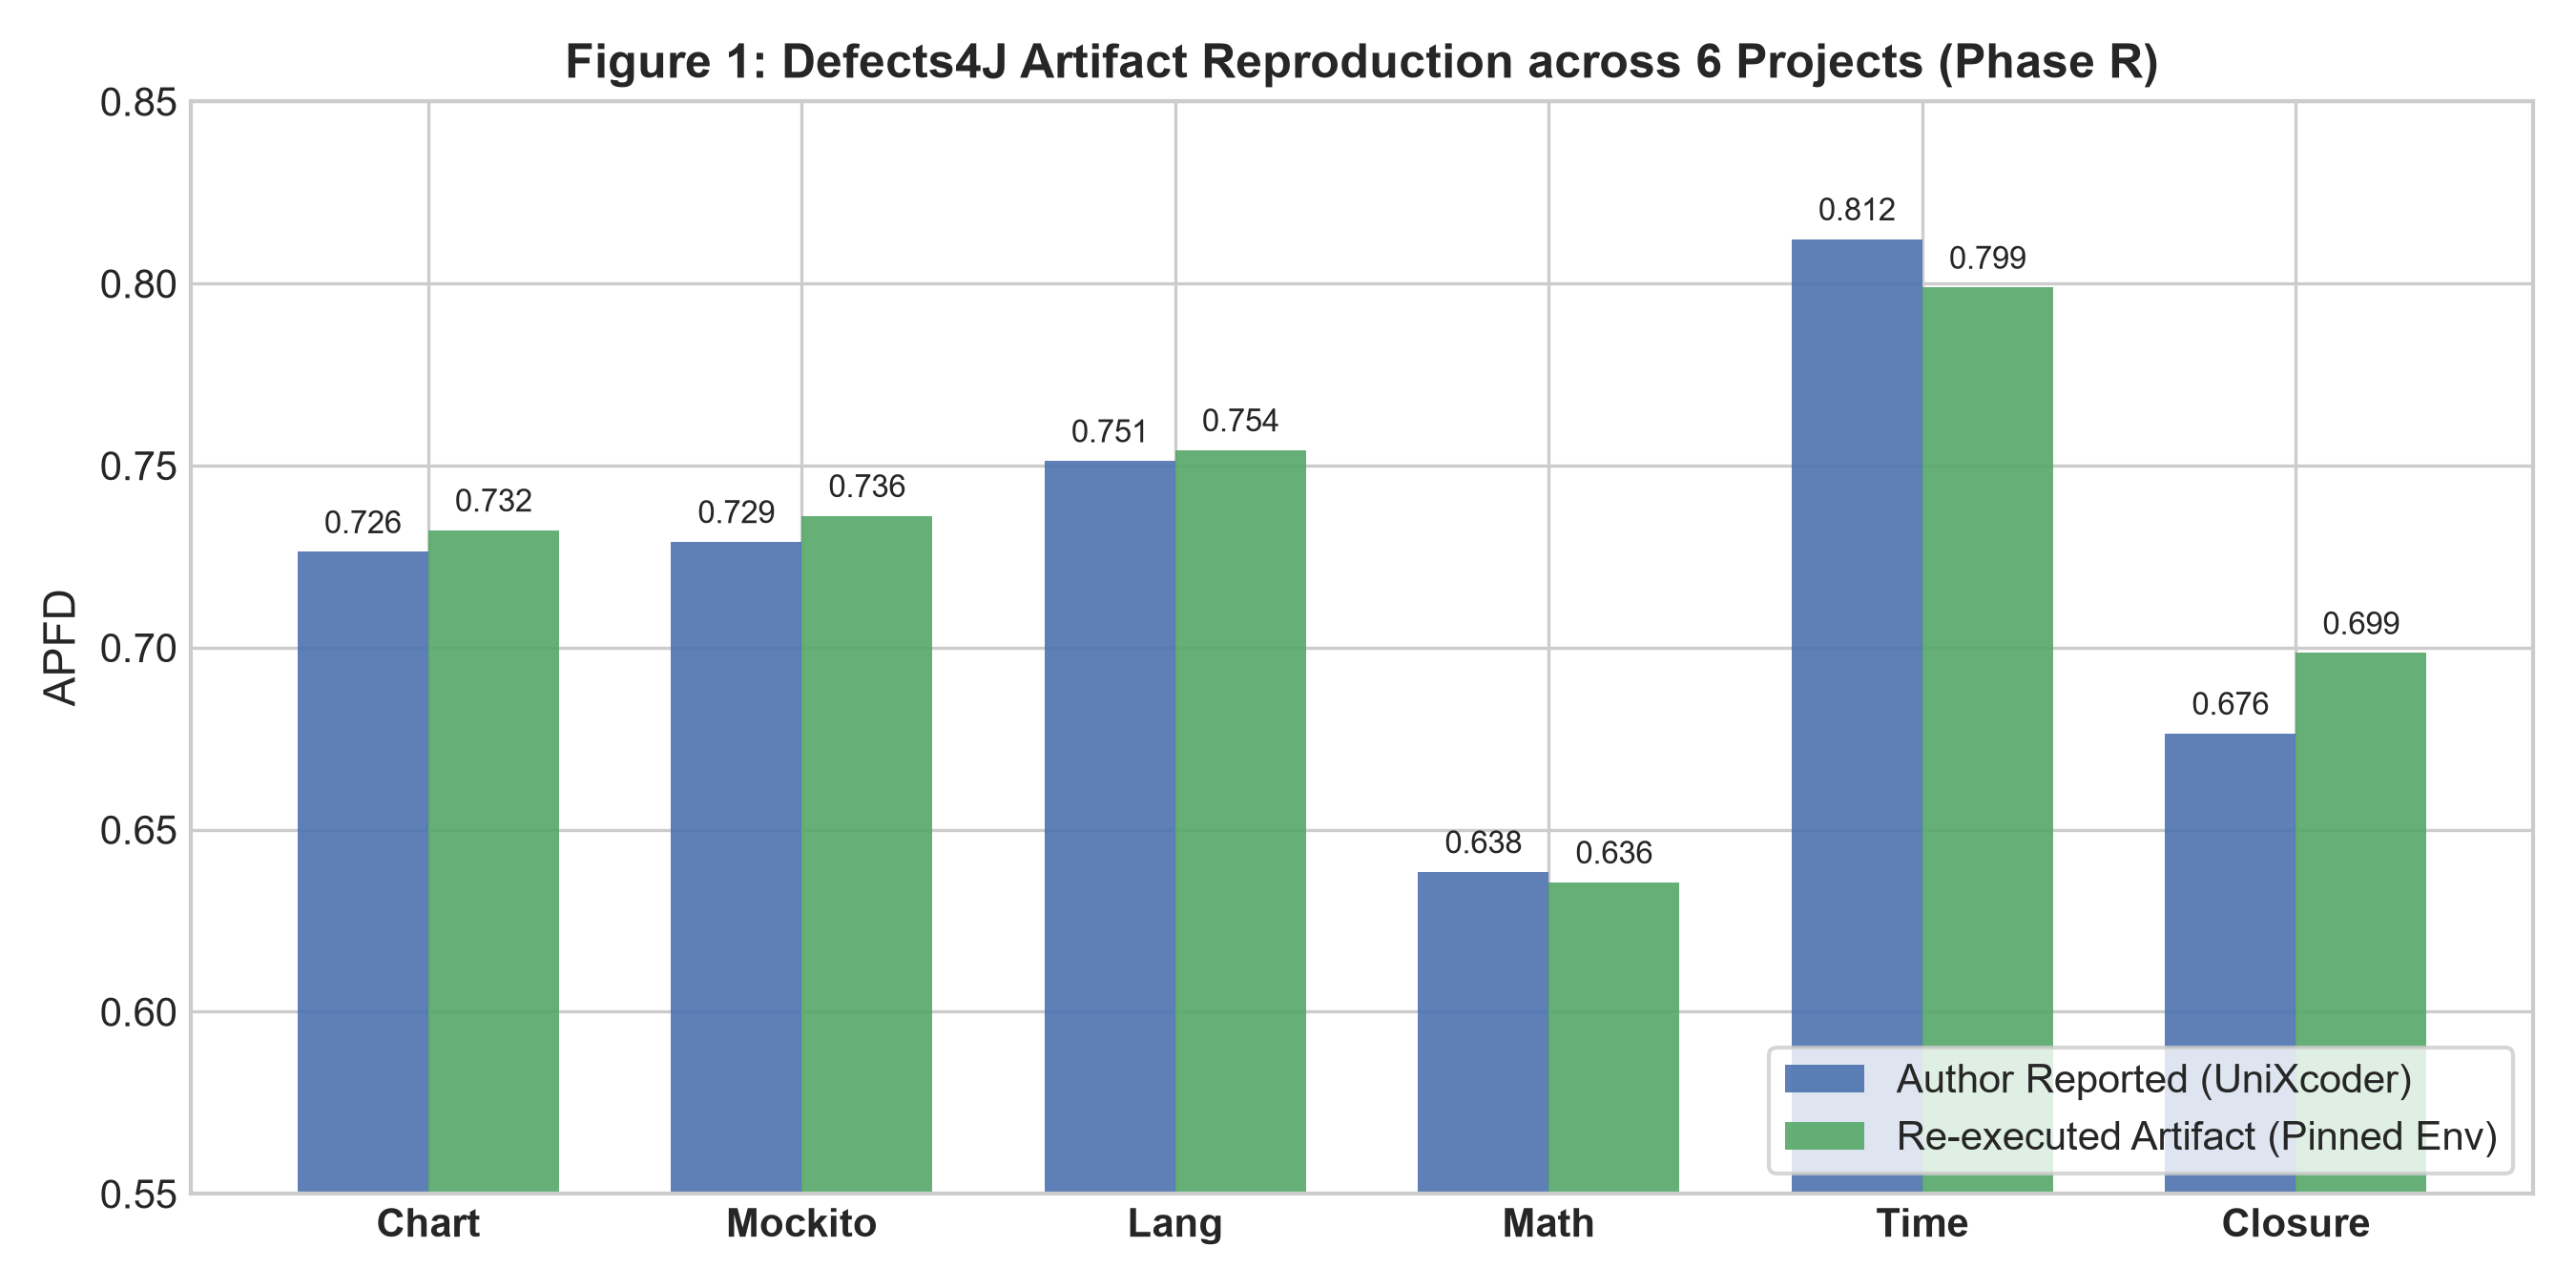
\includegraphics[width=0.85\textwidth]{Images/Figs/fig1_defects4j_reproduction.png}
\caption{So sánh điểm APFD giữa bài báo gốc FALCON và kết quả tái lập trên 6 dự án Defects4J}
\label{fig:defects4j_reproduction}
\vspace{1mm}
\footnotesize{\textit{Nguồn hình vẽ: Tệp kết xuất đồ họa \texttt{reports/figures/fig1\_defects4j\_reproduction.png}.}}
\end{figure}

% -----------------------------------------------------------------------------
\subsubsection{Phân tích phân rã kỹ thuật Bridge trên dự án Chart}
\label{subsubsec:bridge_chart}

Để xác định chính xác các yếu tố kỹ thuật tạo ra sự chênh lệch nhỏ trong tái lập, một thử nghiệm phân tách cấu trúc (Bridge experiment) gồm 4 nhánh (Arms) đã được thiết kế trên dự án Chart (26 phiên bản lỗi):
\begin{itemize}
    \item \textbf{Arm A (Base Pipeline):} Cài đặt cơ sở bám sát mô tả trong bài báo, không sử dụng clipping độ tương đồng.
    \item \textbf{Arm B (Cosine Clipping):} Cắt tỉa giá trị tương đồng cosin về khoảng $[0, 1]$ để ngăn ngừa giá trị âm.
    \item \textbf{Arm C (Greedy Sorting Variant):} Thay đổi quy tắc phá vỡ thế hòa (tie-breaking) trong thuật toán Greedy.
    \item \textbf{Arm D (Full Preprocessing Pipeline + Attention Mask):} Áp dụng tiền xử lý mã nguồn đầy đủ và sử dụng mặt nạ chú ý (attention mask) chuẩn của UniXcoder.
\end{itemize}

% nguon: reports/stage10/bridge/summary.json
Bảng~\ref{tab:bridge_chart_results} trình bày kết quả APFD thu được trên từng nhánh của thử nghiệm Bridge.

\begin{table}[H]
\centering
\caption{Kết quả phân rã các yếu tố kỹ thuật trong thử nghiệm Bridge trên dự án Chart}
\label{tab:bridge_chart_results}
\small
\begin{tabular}{llr}
\toprule
\textbf{Nhánh thử nghiệm} & \textbf{Cấu hình kỹ thuật} & \textbf{APFD trung bình} \\
\midrule
% nguon: reports/stage10/bridge/summary.json
Arm A & Base pipeline (không clipping) & 0,7323 \\
Arm B & Bổ sung Cosine Clipping $[0, 1]$ & 0,7323 \\
Arm C & Thay đổi quy tắc tie-breaking Greedy & 0,7323 \\
Arm D & Tiền xử lý mã nguồn + Attention Mask chuẩn & \textbf{0,7635} \\
\bottomrule
\end{tabular}
\vspace{1mm}\\
\footnotesize{\textit{Nguồn dữ liệu: Trích xuất từ tệp \texttt{reports/stage10/bridge/summary.json}. Chênh lệch giữa Arm D và Arm A đạt $+0,0312$ (+3,12 điểm phần trăm).}}
\end{table}

% nguon: reports/stage10/bridge/summary.json
Số liệu từ Bảng~\ref{tab:bridge_chart_results} ghi nhận điểm APFD trung bình giữ nguyên mức 0,7323 khi áp dụng clipping ma trận tương đồng (Arm B) hoặc thay đổi thứ tự phá vỡ thế hòa (Arm C). Tại nhánh Arm D (kết hợp tiền xử lý mã nguồn và mặt nạ chú ý chuẩn), điểm APFD trung bình đạt \textbf{0,7635}, tương ứng mức chênh lệch $+0,0312$ (+3,12 điểm phần trăm) so với Arm A.

Hình~\ref{fig:chart_bridge} thể hiện diễn biến điểm số qua 4 cấu hình của thử nghiệm Bridge.

\begin{figure}[H]
\centering
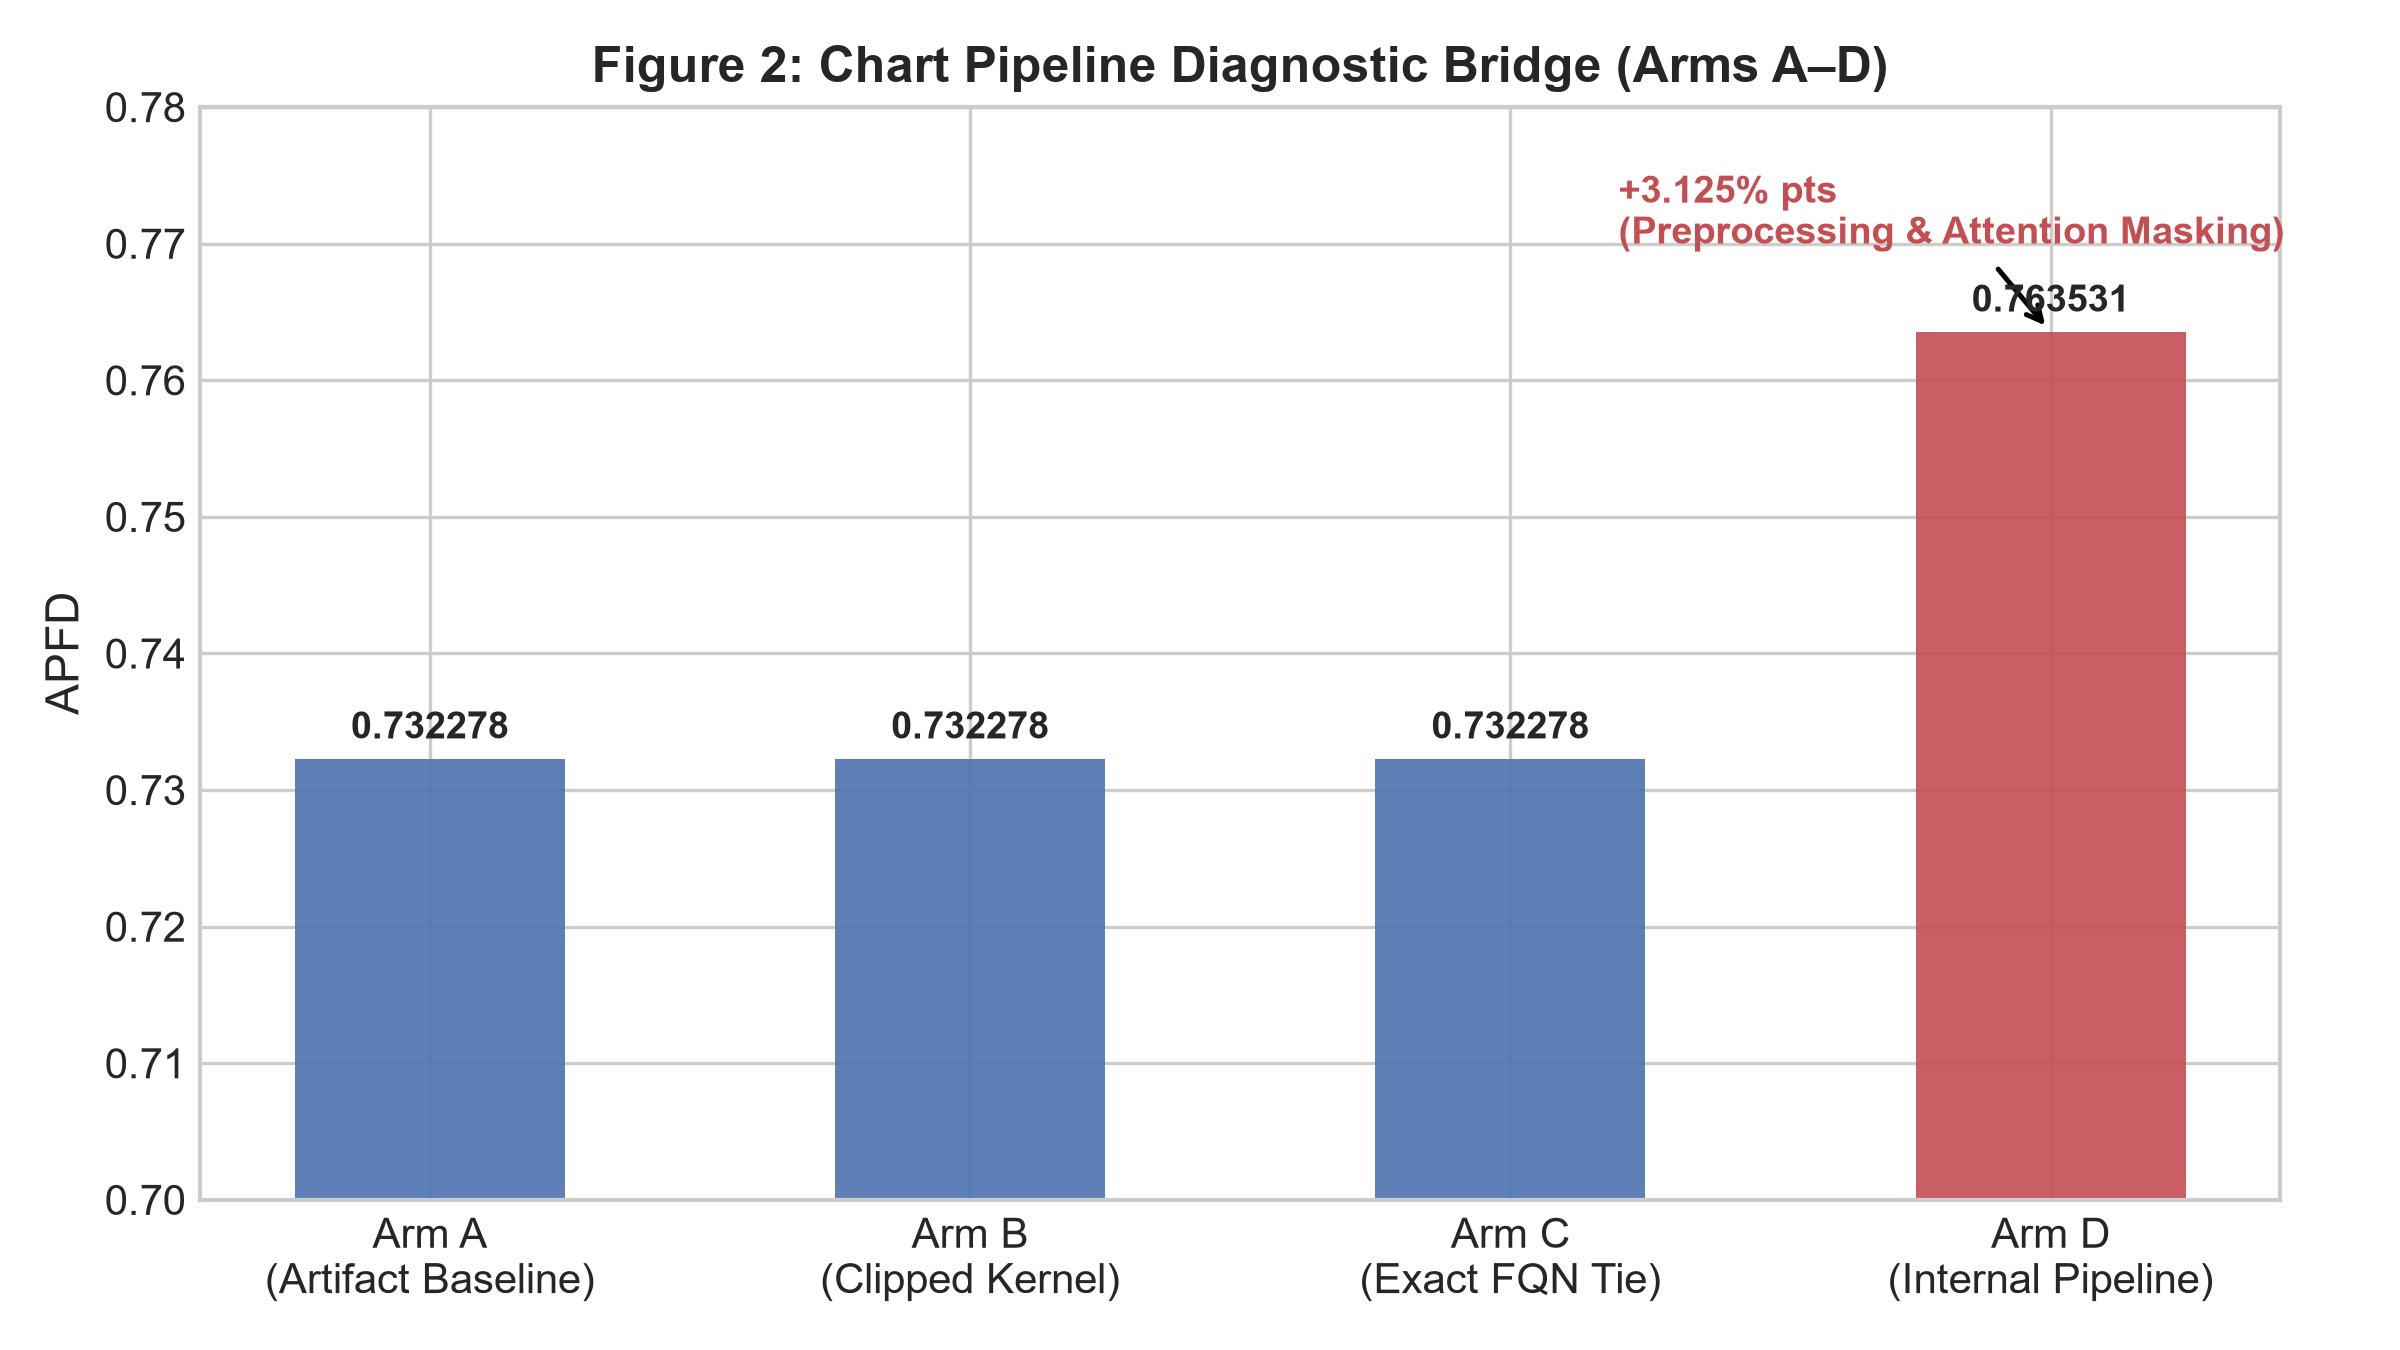
\includegraphics[width=0.85\textwidth]{Images/Figs/fig2_chart_bridge.png}
\caption{Phân rã ảnh hưởng của các thành phần kỹ thuật (Arm A--D) trên dự án Chart}
\label{fig:chart_bridge}
\vspace{1mm}
\footnotesize{\textit{Nguồn hình vẽ: Tệp kết xuất đồ họa \texttt{reports/figures/fig2\_chart\_bridge.png}.}}
\end{figure}

% -----------------------------------------------------------------------------
\subsubsection{Phát hiện kỹ thuật về Attention Mask}
\label{subsubsec:attention_mask_finding}

% nguon: reports/stage10/bridge/summary.json
Đối chiếu cấu hình giữa các nhánh thử nghiệm xác nhận sự thay đổi điểm số chỉ xuất hiện tại Arm D khi tích hợp tiền xử lý mã nguồn và truyền mặt nạ chú ý (attention mask) vào mô hình UniXcoder. Toàn bộ các thảo luận và phân tích cơ chế tác động của biểu diễn vector được trình bày tại Chương~\ref{sec:discussion}.

% =============================================================================
\subsection{Kết quả Trục 2: HC-FALCON trên hệ thống CI thực tế (LRTS)}
\label{subsec:rq2_lrts_results}

% -----------------------------------------------------------------------------
\subsubsection{Mốc đối chứng cơ sở ngẫu nhiên trên chuỗi thời gian CI}
\label{subsubsec:random_baseline_lrts}

% nguon: reports/stage6/karaf/summary.json, reports/stage6/activemq/summary.json, reports/stage6/log4j/summary.json, reports/stage12/ugcs_v2_absolute_apfdc.json
Trên tập Sàng lọc Phát triển (161 build lỗi), đường cơ sở ngẫu nhiên (\texttt{random}, trung bình qua 20 hạt giống ngẫu nhiên) ghi nhận điểm APFDc trung bình lần lượt là \textbf{0,4936} (trung vị 0,4908) tại Apache Karaf ($N=79$), \textbf{0,4945} (trung vị 0,4876) tại Apache ActiveMQ ($N=57$) và \textbf{0,4835} (trung vị 0,4897) tại Apache Log4j2 ($N=25$). Đường cơ sở thuần ngữ nghĩa (\texttt{fl\_only}) đạt điểm APFDc trung bình lần lượt là 0,4558 (Karaf), 0,5182 (ActiveMQ) và 0,6062 (Log4j2).

Bảng~\ref{tab:lrts_baseline_comparison} đối chiếu điểm APFDc trung bình giữa các đường cơ sở và các biến thể chính của đề tài trên chuỗi thời gian CI.

\begin{table}[H]
\centering
\caption{Đối chiếu điểm APFDc trung bình giữa các đường cơ sở và các biến thể chính trên CI}
\label{tab:lrts_baseline_comparison}
\small
\begin{adjustbox}{max width=\textwidth}
\begin{tabular}{lrrrr}
\toprule
\textbf{Phương pháp / Đường cơ sở} & \textbf{Karaf ($N=79$)} & \textbf{ActiveMQ ($N=57$)} & \textbf{Log4j2 ($N=25$)} & \textbf{Toàn bộ ($N=161$)} \\
\midrule
% nguon: reports/stage6/karaf/summary.json, reports/stage6/activemq/summary.json, reports/stage6/log4j/summary.json
Cơ sở ngẫu nhiên (\texttt{random})    & 0,4936 & 0,4945 & 0,4835 & 0,4923 \\
Thuần ngữ nghĩa (\texttt{fl\_only})   & 0,4558 & 0,5182 & 0,6062 & 0,5013 \\
Đường cơ sở \texttt{history\_cost}    & 0,7754 & 0,8486 & 0,8936 & 0,8197 \\
\midrule
% nguon: reports/release/statistical_tests_all_gens.json
HC-FALCON v1 (\texttt{normalized})   & 0,7710 & 0,8147 & 0,9014 & 0,8067 \\
% nguon: reports/stage12/ugcs_v2_absolute_apfdc.json
UGCS v2 (\texttt{hc\_ugcs\_v2})$^{*}$ & \textbf{0,7802} & \textbf{0,8471} & \textbf{0,8952} & \textbf{0,8217} \\
\bottomrule
\end{tabular}
\end{adjustbox}
\vspace{1mm}\\
\footnotesize{\textit{Nguồn dữ liệu: Tệp tổng hợp \texttt{reports/stage6/*/summary.json}, \texttt{reports/release/statistical\_tests\_all\_gens.json} và \texttt{reports/stage12/ugcs\_v2\_absolute\_apfdc.json}. ($*$) Điểm APFDc tuyệt đối của UGCS v2 được suy ra trực tiếp từ chênh lệch ghép cặp theo từng build vật lý: $\text{APFDc}(\text{UGCS v2})_i = \text{APFDc}(\text{history\_cost})_i + \Delta_i$.}}
\end{table}

Để so sánh đối chứng, biến thể khởi đầu HC-FALCON v1 (\texttt{normalized}) đạt điểm APFDc trung bình là \textbf{0,7710} tại Karaf, \textbf{0,8147} tại ActiveMQ và \textbf{0,9014} tại Log4j2; đường cơ sở \texttt{history\_cost} đạt điểm APFDc trung bình là \textbf{0,7754} tại Karaf, \textbf{0,8486} tại ActiveMQ và \textbf{0,8936} tại Log4j2. Biến thể cuối UGCS v2 đạt điểm APFDc trung bình suy ra lần lượt là \textbf{0,7802} tại Karaf, \textbf{0,8471} tại ActiveMQ và \textbf{0,8952} tại Log4j2 (trung bình toàn cục đạt \textbf{0,8217}). Mặc dù điểm APFDc trung bình của UGCS v2 tương đương \texttt{history\_cost}, việc phân tích kiểm định ghép cặp chi tiết theo từng bản build tại Mục~\ref{subsubsec:stage12_results} chỉ ra rằng UGCS v2 vẫn thua \texttt{history\_cost} ở 72,05\% số build vật lý.

% -----------------------------------------------------------------------------
\subsubsection{Diễn tiến các biến thể từ HC-FALCON v1 đến CNS-Greedy}
\label{subsubsec:variants_evolution}

Quá trình nghiên cứu trên tập Sàng lọc Phát triển (161 build lỗi) đã trải qua 4 thế hệ thuật toán liên tiếp:
\begin{enumerate}
    \item \textbf{Thế hệ 1 -- HC-FALCON v1 (Stage 6):} Bao gồm hai biến thể kết hợp tuyến tính giữa hàm Facility Location và trọng số lịch sử: dạng trọng số thô (\texttt{topic\_raw}) và dạng chuẩn hóa (\texttt{normalized}).
    % nguon: reports/release/statistical_tests.json (dòng 10, 25, 40)
    Biến thể chuẩn hóa ghi nhận trung vị $\Delta\text{APFDc}$ so với \texttt{history\_cost} lần lượt là $-1,2650$ điểm phần trăm (Karaf), $-1,4067$ điểm phần trăm (ActiveMQ) và $-0,1171$ điểm phần trăm (Log4j2).
    % nguon: reports/stage11/forensic-analysis.json (dòng 651-654)
    Trên toàn bộ 161 build lỗi, HC-FALCON v1 chỉ thắng 38 build (23,6\%), hòa 1 build (0,6\%) và thua 122 build (75,8\%).
    \item \textbf{Thế hệ 2 -- Hạn chế ngữ nghĩa theo cửa sổ lịch sử (Stage 8):} Giới hạn không gian tìm kiếm tham lam trong cửa sổ động theo từng bước với $q_b(i) \ge 0{,}95 \cdot q_b(t^*)$ và $c_b(i) \le 1{,}25 \cdot c_b(t^*)$ (neo theo phần tử đầu baseline $t^*$).
    % nguon: reports/stage8/summary.json
    Biến thể này ghi nhận: tại Karaf đạt 13 thắng / 17 hòa / 49 thua (trung vị $\Delta = -0,0171$ điểm phần trăm); tại ActiveMQ đạt 13 thắng / 1 hòa / 43 thua (trung vị $\Delta = -0,1537$ điểm phần trăm); tại Log4j2 đạt 5 thắng / 6 hòa / 14 thua (trung vị $\Delta = -0,0008$ điểm phần trăm). Tổng cộng trên 161 build lỗi, biến thể đạt 31 thắng / 24 hòa / 106 thua (thua 65,84\%).
    \item \textbf{Thế hệ 3 -- CNS-Greedy (Stage 11):} Can thiệp trực tiếp vào lợi ích biên kết hợp qua công thức $\text{gain}_{\text{CNS}}(i \mid S) = \alpha \cdot \frac{\Delta FL_b(i \mid S)}{n \cdot \sqrt{\max\left(c_b(i), \, 10^{-6}\right)}} + (1 - \alpha) \cdot w_b(i)$ với thời lượng thô $c_b(i)$ tính bằng giây và trọng số lịch sử chuẩn hóa $w_b(i) = q_b(i) / \sum q$.
    % nguon: reports/release/statistical_tests_all_gens.json (mục hc_cns_v1)
    Trên 161 build lỗi, CNS-Greedy đạt 22 thắng / 1 hòa / 56 thua tại Karaf (trung vị $\Delta = -0,3994$ điểm phần trăm), 10 thắng / 0 hòa / 47 thua tại ActiveMQ (trung vị $\Delta = -0,6064$ điểm phần trăm) và 6 thắng / 0 hòa / 19 thua tại Log4j2 (trung vị $\Delta = -0,1896$ điểm phần trăm). Tổng cộng đạt 38 thắng / 1 hòa / 122 thua (thua 75,78\%).
    \item \textbf{Thế hệ 4 -- UGCS v2 (Stage 12):} Biến thể tiền đăng ký kết hợp 4 công đoạn: Ước lượng Bayes $\to$ Khoanh vùng bất định $\to$ Tham lam có ý thức chi phí $\to$ Tie-breaking.
    % nguon: reports/stage12/stage12_statistical_tests_paired_effect_sizes.json
    Kết quả kiểm định ghi nhận: 20 thắng / 4 hòa / 55 thua tại Karaf (trung vị $\Delta = -0,0586$ điểm phần trăm), 9 thắng / 4 hòa / 44 thua tại ActiveMQ (trung vị $\Delta = -0,2235$ điểm phần trăm) và 6 thắng / 2 hòa / 17 thua tại Log4j2 (trung vị $\Delta = -0,0017$ điểm phần trăm). Tổng cộng đạt 35 thắng / 10 hòa / 116 thua (thua 72,05\%).
\end{enumerate}

% nguon: reports/stage12/winning_builds_intersection.json
Đối soát giao thoa các tập build thắng giữa các thế hệ thuật toán xác nhận:
\begin{itemize}
    \item \textbf{Giữa Stage 6 (v1) và Stage 8 (Hạn chế ngữ nghĩa):} Stage 8 giữ lại 15 trong số 38 ca thắng của v1 (39,5\%), đồng thời mở ra thêm 16 ca thắng mới mà v1 không đạt được. Số liệu này bác bỏ giả thuyết cho rằng Stage 8 bóp nghẹt toàn bộ các ca thắng của v1.
    \item \textbf{Giữa Stage 6 (v1) và Stage 11 (CNS-Greedy):} Mặc dù cả hai biến thể cùng đạt chính xác 38 build thắng trên toàn bộ 161 build lỗi, hai tập hợp build thắng này không trùng khớp nhau ($\text{Wins}_{v1} \neq \text{Wins}_{\text{cns}}$). Chúng chỉ giao thoa 23 build chung (60,5\%), mỗi biến thể sở hữu 15 ca thắng độc lập còn lại.
    \item \textbf{Tính bền vững qua 4 thế hệ:} Có đúng 14 build lỗi duy trì được chiến thắng trước \texttt{history\_cost} xuyên suốt từ biến thể khởi đầu v1 tới biến thể cuối UGCS v2.
\end{itemize}

% -----------------------------------------------------------------------------
\subsubsection{Kết quả của biến thể cuối UGCS v2 (Stage 12)}
\label{subsubsec:stage12_results}

Bảng~\ref{tab:stage12_comprehensive} trình bày chi tiết kết quả kiểm định thống kê và các chỉ số kích thước hiệu ứng của biến thể cuối UGCS v2 so với đường cơ sở \texttt{history\_cost} trên tập Sàng lọc Phát triển.

\begin{table}[H]
\centering
\caption{Kết quả kiểm định thống kê ghép cặp giữa UGCS v2 và baseline \texttt{history\_cost}}
\label{tab:stage12_comprehensive}
\begin{adjustbox}{max width=\textwidth}
\small
\begin{tabular}{lrrr}
\toprule
\textbf{Chỉ số thống kê} & \textbf{Apache Karaf} & \textbf{Apache ActiveMQ} & \textbf{Apache Log4j2} \\
\midrule
% nguon: reports/stage12/stage12_statistical_tests_paired_effect_sizes.json
Số lượng physical build lỗi ($N$) & 79 & 57 & 25 \\
Số build Thắng / Thua / Hòa & 20 / 55 / 4 & 9 / 44 / 4 & 6 / 17 / 2 \\
Tỷ lệ thắng (Win rate) & 25,32\% & 15,79\% & 24,00\% \\
\midrule
% nguon: reports/stage12/stage12_statistical_tests.json
Trung vị chênh lệch ($\text{Median}(\Delta)$, điểm phần trăm) & \textbf{$-0,0586$} & \textbf{$-0,2235$} & \textbf{$-0,0017$} \\
Trung bình chênh lệch ($\text{Mean}(\Delta)$, điểm phần trăm)   & \textbf{$+0,4788$} & \textbf{$-0,1508$} & \textbf{$+0,1663$} \\
Khoảng tin cậy Bootstrap 95\% (điểm phần trăm) & [$-0,2659, +1,4488$] & [$-0,8112, +0,6703$] & [$-0,1606, +0,6060$] \\
\midrule
% nguon: reports/stage12/stage12_statistical_tests.json
Wilcoxon $W$-statistic & 1.067,0 & 318,0 & 113,0 \\
Giá trị $p$ chưa hiệu chỉnh ($p_{\text{raw}}$) & 0,012684 & $6,30 \times 10^{-5}$ & 0,187317 \\
Giá trị $p$ hiệu chỉnh Holm ($p_{\text{holm}}$) & \textbf{0,025368} & \textbf{0,000189} & \textbf{0,187317} \\
\midrule
% nguon: reports/stage12/stage12_statistical_tests_paired_effect_sizes.json
Paired Cliff's delta ($\delta_{\text{paired}}$) & \textbf{$-0,4430$} & \textbf{$-0,6140$} & \textbf{$-0,4400$} \\
Rank-biserial correlation ($r_{rb}$) & \textbf{$-0,3102$} & \textbf{$-0,6059$} & \textbf{$-0,2681$} \\
\bottomrule
\end{tabular}
\end{adjustbox}
\vspace{1mm}\\
\footnotesize{\textit{Nguồn dữ liệu: Tệp kiểm định \texttt{reports/stage12/stage12\_statistical\_tests\_paired\_effect\_sizes.json}. Chú ý thống kê: Trung vị của hiệu khác hiệu của các trung vị ($\text{Median}(X - Y) \neq \text{Median}(X) - \text{Median}(Y)$). Do đó, việc trung vị chênh lệch ghép cặp $\text{Median}(\Delta)$ mang dấu âm (do đa số các build có hiệu âm) hoàn toàn tương thích về mặt toán học với việc hiệu của hai trung vị mẫu hoặc giá trị trung bình $\text{Mean}(\Delta)$ mang dấu dương (bị chi phối bởi một số ít build có mức chênh lệch dương lớn).}}
\end{table}

Số liệu từ Bảng~\ref{tab:stage12_comprehensive} chỉ ra các hiện tượng thống kê cụ thể:
\begin{enumerate}
    \item \textbf{Hiện tượng phân kỳ dấu giữa Median và Mean tại Apache Karaf:}
    % nguon: reports/stage12/stage12_statistical_tests.json
    Tại Karaf, giá trị trung vị chênh lệch mang dấu âm ($-0,0586$ điểm phần trăm, với 20 build thắng, 55 build thua và 4 build hòa), trong khi giá trị trung bình chênh lệch mang dấu dương ($+0,4788$ điểm phần trăm). Cần nhấn mạnh nguyên lý thống kê: trung vị của hiệu khác hiệu của các trung vị ($\text{Median}(\Delta) \neq \text{Median}_{\text{cand}} - \text{Median}_{\text{base}}$). Khoảng tin cậy Bootstrap 95\% của giá trị trung bình trải rộng từ $-0,2659$ đến $+1,4488$ điểm phần trăm (chứa mốc 0), cho thấy sự khác biệt trung bình không đạt ý nghĩa thống kê ở mức $\alpha = 0,05$.
    \item \textbf{Mức độ thua thiệt tại Apache ActiveMQ:}
    Tại ActiveMQ, cả trung vị ($-0,2235$ điểm phần trăm) và trung bình ($-0,1508$ điểm phần trăm) đều mang dấu âm, với tỷ lệ thắng chỉ đạt 15,79\% (9 thắng vs 44 thua). Kiểm định Wilcoxon đạt mức ý nghĩa thống kê rất cao ($p_{\text{holm}} = 0,000189 < 0,001$). Các chỉ số kích thước hiệu ứng ghép cặp ghi nhận mức bất lợi lớn: Paired Cliff's delta đạt $-0,6140$ và Rank-biserial đạt $-0,6059$.
    \item \textbf{Thiếu ý nghĩa thống kê tại Apache Log4j2:}
    Tại Log4j2 ($N=25$), tỷ số thắng/thua là 6/17, trung vị đạt $-0,0017$ điểm phần trăm, giá trị $p$ hiệu chỉnh Holm đạt 0,187317 ($> 0,05$) và khoảng tin cậy 95\% chứa mốc 0 ([$-0,1606, +0,6060$] điểm phần trăm).
\end{enumerate}

Hình~\ref{fig:lrts_effect_gate} minh họa phân phối chênh lệch ghép cặp $\Delta\text{APFDc}$ của UGCS v2 so với hai đường cơ sở đối chứng trên cả 3 dự án.

\begin{figure}[H]
\centering
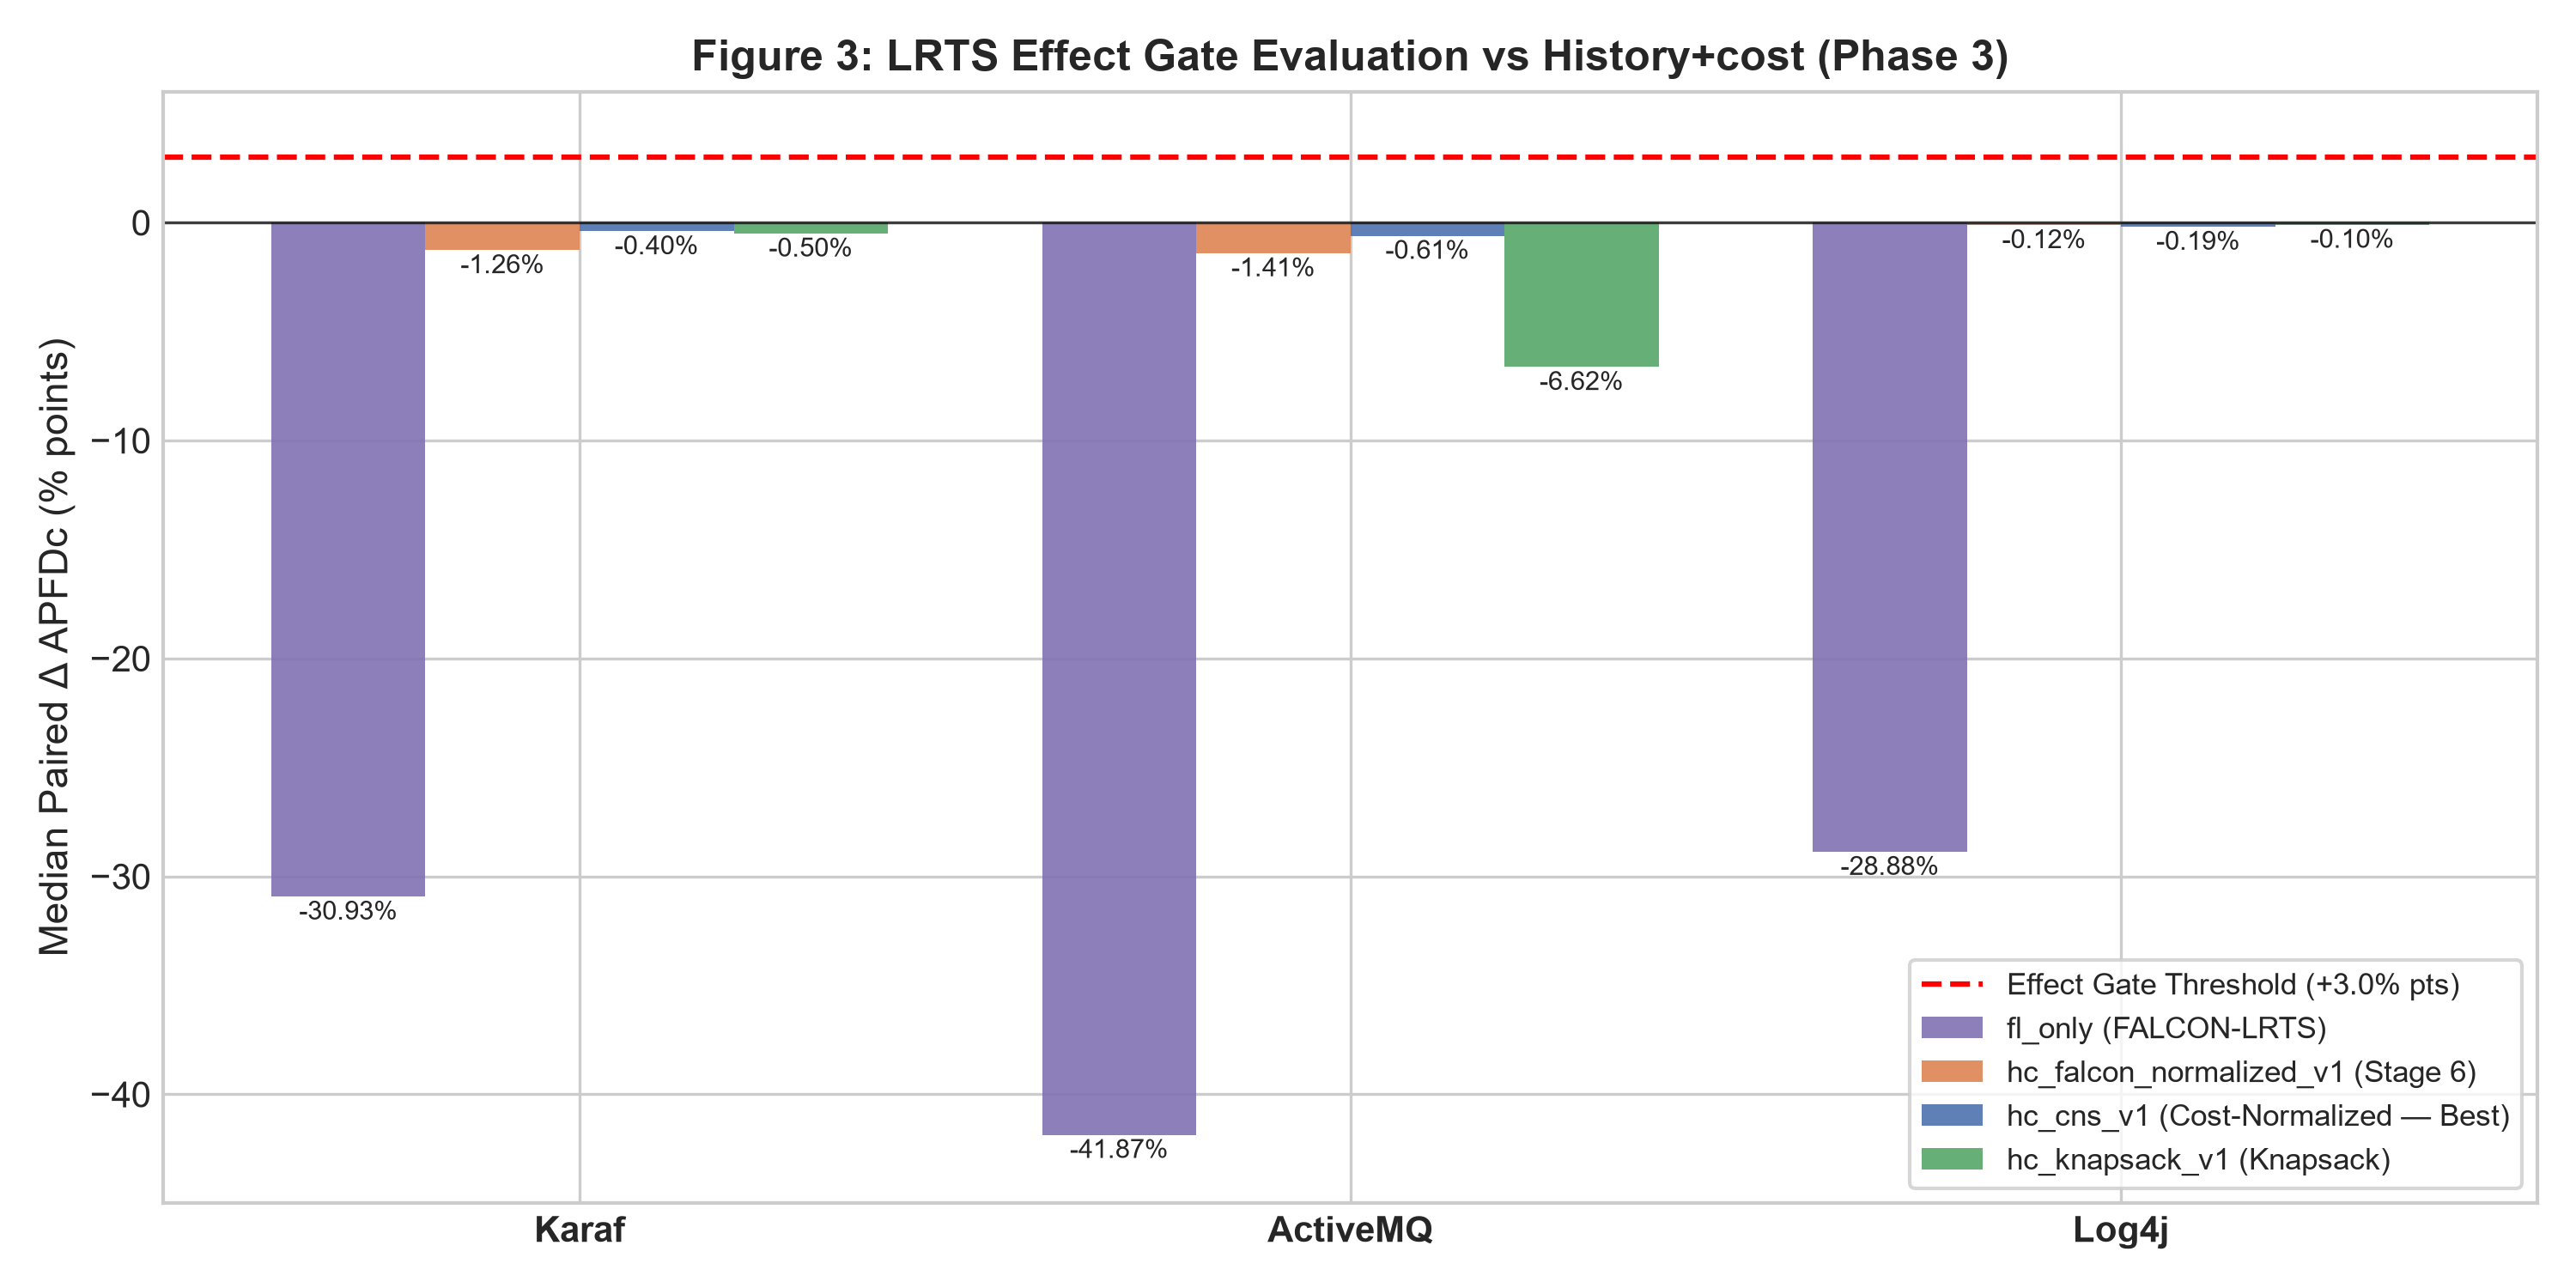
\includegraphics[width=0.85\textwidth]{Images/Figs/fig3_lrts_effect_gate.png}
\caption[Phân phối chênh lệch ghép cặp $\Delta\text{APFDc}$ của UGCS v2 so với các baseline]{Phân phối chênh lệch ghép cặp $\Delta\text{APFDc}$ của UGCS v2 so với \texttt{history\_cost} và \texttt{fl\_only}}
\label{fig:lrts_effect_gate}
\vspace{1mm}
\footnotesize{\textit{Nguồn hình vẽ: Tệp kết xuất đồ họa \texttt{reports/figures/fig3\_lrts\_effect\_gate.png}. Đường nét đứt màu đỏ biểu thị ngưỡng yêu cầu $+3,0$ điểm phần trăm của Effect Gate.}}
\end{figure}

% -----------------------------------------------------------------------------
\subsubsection{Đánh giá các chỉ tiêu kỹ thuật (Overhead thời gian và Bộ nhớ)}
\label{subsubsec:engineering_metrics}

% nguon: reports/stage12/development-screen.json (dòng 85-113)
Bên cạnh hiệu quả phát hiện lỗi, đề tài đã tiến hành đo đạc chính xác các chỉ tiêu kỹ thuật thực thi của UGCS v2 so với đường cơ sở \texttt{history\_cost} trên toàn bộ 171 stage thuộc 161 build lỗi của tập Sàng lọc Phát triển:
\begin{itemize}
    % nguon: reports/stage12/development-screen.json (dòng 111, 112)
    \item \textbf{Độ trễ tính toán mỗi stage (Latency per stage):} Baseline nhẹ \texttt{history\_cost} có thời gian xếp hạng cực nhanh với độ trễ trung vị chỉ \textbf{0,11 ms} ($0,0001126$ giây). Ngược lại, việc giải bài toán chọn tập con tham lam có nhận thức chi phí kết hợp nhân cosin ngữ nghĩa của UGCS v2 đòi hỏi độ trễ trung vị là \textbf{53,82 ms} ($0,053819$ giây), tức chậm hơn xấp xỉ 478 lần ở mức trung vị.
    % nguon: reports/stage12/development-screen.json (dòng 89, 109)
    \item \textbf{Tỷ lệ overhead trần ở phân vị P95 (P95 warm overhead fraction):} Tỷ lệ gia tăng chi phí thời gian xếp hạng ở phân vị thứ 95 của UGCS v2 so với \texttt{history\_cost} lên tới \textbf{14.257,90 lần} ($+1.425.790\%$). Mức overhead tính toán vượt xa ngưỡng trần cho phép $+10\%$ ($0,10$), dẫn tới việc phương pháp vi phạm hoàn toàn Runtime Gate.
    % nguon: reports/stage12/development-screen.json (dòng 95, 110)
    \item \textbf{Mức chiếm dụng bộ nhớ đỉnh (Peak RSS):} Mức tiêu thụ bộ nhớ RAM cao nhất của tiến trình xếp hạng ghi nhận tại \textbf{656,4 MiB} ($688.287.744$ bytes), nằm an toàn dưới ngưỡng trần tiền đăng ký là 8,0 GiB ($8.589.934.592$ bytes).
    \item \textit{Ghi chú đối soát dữ liệu:} Các phân vị cụ thể khác (P95 tuyệt đối, Max) của thời gian chạy từng build vật lý cũng như của biến thể HC-FALCON v1 không xác định được từ tệp \texttt{reports/stage12/development-screen.json} do tệp nguồn chỉ lưu trữ trung vị độ trễ của hai phương pháp và tỷ lệ trần P95 toàn cục.
\end{itemize}

% -----------------------------------------------------------------------------
\subsubsection{Phán quyết thẩm định theo tiêu chí tiền đăng ký}
\label{subsubsec:preregistered_decision}

% nguon: reports/stage12/development-screen.json (dòng 10-104), configs/hc-falcon-v2-preregistered.json (dòng 42-69)
Bảng~\ref{tab:decision_gates_evaluation} tổng hợp kết quả đối chiếu toàn bộ 4 cổng quyết định tiền đăng ký đối với biến thể cuối UGCS v2 trên tập Sàng lọc Phát triển.

\begin{table}[H]
\centering
\caption{Đánh giá các cổng quyết định tiền đăng ký (Decision Gates) đối với biến thể UGCS v2}
\label{tab:decision_gates_evaluation}
\small
\begin{adjustbox}{max width=\textwidth}
\begin{tabular}{llp{5.5cm}ll}
\toprule
\textbf{Cổng thẩm định} & \textbf{Chỉ số đánh giá} & \textbf{Ngưỡng tiền đăng ký} & \textbf{Giá trị quan sát} & \textbf{Kết luận} \\
\midrule
% nguon: reports/stage12/development-screen.json (dòng 15-20)
Effect Gate      & $\Delta\text{APFDc}$ vs baseline & $\ge +3,0$ điểm phần trăm trên $\ge 2/3$ dự án so với \texttt{history\_cost} và \texttt{fl\_only} & 0/3 dự án đạt chuẩn so với \texttt{history\_cost} & \textbf{KHÔNG ĐẠT} \\
% nguon: reports/stage12/development-screen.json (dòng 86-90)
Runtime Gate     & Overhead thời gian P95          & Tỷ lệ gia tăng chi phí $\le 0,10$ ($+10\%$) vs \texttt{history\_cost} & $14.257,90\times$ ($+1.425.790\%$) & \textbf{VI PHẠM} \\
% nguon: reports/stage12/development-screen.json (dòng 92-96)
Memory Gate      & Mức chiếm dụng đỉnh (Peak RSS)   & Dung lượng RAM $\le 8{,}0$ GiB ($8.589.934.592$ bytes) & 656,4 MiB ($688.287.744$ bytes) & \textbf{ĐẠT} \\
% nguon: reports/stage12/development-screen.json (dòng 98-102)
Audit Gate       & Tính toàn vẹn và lỗi thực thi   & Hoàn thành 171 stage trên 161 build, không có lỗi & 171/171 stage, 0 lỗi audit & \textbf{ĐẠT} \\
\midrule
% nguon: reports/stage12/development-screen.json (dòng 10, 7)
\textbf{Phán quyết chung} & \textbf{Quyết định phát hành} & \textbf{Vượt qua toàn bộ 4 cổng} & \textbf{Vi phạm 2/4 cổng} & \textbf{NO-GO} \\
\bottomrule
\end{tabular}
\end{adjustbox}
\vspace{1mm}\\
\footnotesize{\textit{Nguồn dữ liệu: Tệp thẩm định chính thức \texttt{reports/stage12/development-screen.json}.}}
\end{table}

% nguon: docs/12-hc-falcon-v2/evaluation-protocol.md (dòng 104-117)
Đối chiếu với các điều kiện tiền đăng ký, phương pháp đạt 2 cổng kỹ thuật (Memory Gate và Audit Gate) nhưng thất bại tại 2 cổng cốt lõi (Effect Gate và Runtime Gate). Cụ thể, mẫu số chuẩn hóa của chỉ số overhead được quy định nghiêm ngặt là thời gian xếp hạng của đường cơ sở \texttt{history\_cost}:
\begin{equation}
\text{Overhead}_{\text{stage}} = \frac{T_{\text{ugcs}} - T_{\text{hc}}}{\max(T_{\text{hc}}, 10^{-9})}
\end{equation}
Do độ trễ trung vị của \texttt{history\_cost} chỉ là 0,11 ms trong khi UGCS v2 tiêu tốn 53,82 ms, tỷ lệ overhead P95 quan sát lên tới $14.257,90\times$ ($+1.425.790\%$), vượt xa ngưỡng cho phép $+10\%$. Đồng thời, tại Effect Gate, UGCS v2 không đạt mức tăng trưởng $+3,0$ điểm phần trăm so với \texttt{history\_cost} trên bất kỳ dự án nào (0/3 dự án).

Căn cứ theo quy tắc phán quyết đã khóa cứng trước thực nghiệm, kết luận chính thức của đề tài là \textbf{NO-GO}. Hệ thống kích hoạt lệnh đóng băng: \textbf{Toàn bộ 142 build lỗi thuộc tập Xác nhận Niêm phong (Reserved Confirmation) được giữ niêm phong vĩnh viễn (\texttt{reserved\_opened: false})}, bảo đảm tính toàn vẹn phương pháp luận và ngăn ngừa triệt để hiện tượng rò rỉ dữ liệu kiểm chứng.

% =============================================================================
\subsection{Dữ liệu chẩn đoán sâu về hiện tượng Heavy Predecessors}
\label{subsec:rq3_heavy_predecessors}

% -----------------------------------------------------------------------------
\subsubsection{Thống kê độ trễ ròng tích lũy trên 161 build lỗi}
\label{subsubsec:forensic_table}

Để cung cấp bằng chứng thực nghiệm trực tiếp giải thích sự sụt giảm APFDc của các mô hình kết hợp ngữ nghĩa, phân tích điều tra sâu (forensic analysis) đã đo đạc sự dịch chuyển vị trí thực thi của các test class trên toàn bộ 161 build lỗi của biến thể HC-FALCON v1 (\texttt{normalized\_v1}) so với \texttt{history\_cost}.

% nguon: reports/stage12/predecessor_comparison.json, reports/stage11/forensic-analysis.json
Bảng~\ref{tab:heavy_predecessors_breakdown} phân rã chi tiết tổng thời gian các bài test nặng bị đẩy lên trước test lỗi ($T_{add}$), thời gian test lỗi được đẩy lên trước ($T_{rem}$) và độ trễ ròng tích lũy ($T_{net} = T_{add} - T_{rem}$) giữa hai biến thể HC-FALCON v1 và UGCS v2 theo từng dự án. Cả hai biến thể đều được tính toán theo cùng một định nghĩa toán học nhất quán trên 161 build vật lý (171 failing stages) đối chiếu trực tiếp với baseline \texttt{history\_cost}.

\begin{table}[H]
\centering
\caption{Đối chiếu phân rã thời gian trễ do Heavy Predecessors giữa HC-FALCON v1 và UGCS v2}
\label{tab:heavy_predecessors_breakdown}
\small
\begin{adjustbox}{max width=\textwidth}
\begin{tabular}{llrrrrr}
\toprule
\textbf{Biến thể} & \textbf{Dự án CI} & \textbf{Build ($N$)} & \textbf{$T_{add}$ (s)} & \textbf{$T_{rem}$ (s)} & \textbf{$T_{net}$ (s)} & $\mathbf{T_{net}/N}$ \textbf{(s)} \\
\midrule
% nguon: reports/stage12/predecessor_comparison.json (mục hc_falcon_normalized_v1)
\multirow{4}{*}{\textbf{HC-FALCON v1}} 
  & Apache Karaf   & 79 & $+18.205,5$ & $-23.384,8$ & $\mathbf{-5.179,3}$ & $-65,56$ \\
  & Apache ActiveMQ & 57 & $+115.759,2$ & $-71.872,9$ & $\mathbf{+43.886,3}$ & $+769,94$ \\
  & Apache Log4j2  & 25 & $+1.027,2$ & $-635,0$ & $\mathbf{+392,2}$ & $+15,69$ \\
\cmidrule{2-7}
  & \textbf{Tổng cộng v1} & \textbf{161} & $\mathbf{+134.991,9}$ & $\mathbf{-95.892,7}$ & $\mathbf{+39.099,3}$ & $\mathbf{+242,85}$ \\
\midrule
% nguon: reports/stage12/predecessor_comparison.json (mục hc_ugcs_v2)
\multirow{4}{*}{\textbf{UGCS v2}} 
  & Apache Karaf   & 79 & $+4.858,5$ & $-11.378,1$ & $\mathbf{-6.519,6}$ & $-82,53$ \\
  & Apache ActiveMQ & 57 & $+38.644,6$ & $-41.746,1$ & $\mathbf{-3.101,4}$ & $-54,41$ \\
  & Apache Log4j2  & 25 & $+196,2$ & $-206,4$ & $\mathbf{-10,2}$ & $-0,41$ \\
\cmidrule{2-7}
  & \textbf{Tổng cộng UGCS v2} & \textbf{161} & $\mathbf{+43.699,3}$ & $\mathbf{-53.330,6}$ & $\mathbf{-9.631,3}$ & $\mathbf{-59,82}$ \\
\bottomrule
\end{tabular}
\end{adjustbox}
\vspace{1mm}\\
\footnotesize{\textit{Nguồn dữ liệu: Tệp tổng hợp đối soát \texttt{reports/stage12/predecessor\_comparison.json}. Cả hai biến thể được đo đạc bằng cùng một hàm toán học trên 161 build lỗi (171 failing stages). Đối với HC-FALCON v1, tổng độ trễ ròng tích lũy ghi nhận $+39.099,3$ giây; đối với UGCS v2, tổng thời gian ròng ghi nhận mức cắt giảm $-9.631,3$ giây so với \texttt{history\_cost}. Cột $T_{net}/N$ thể hiện độ trễ ròng bình quân trên mỗi bản build vật lý.}}
\end{table}

Số liệu đối chiếu từ Bảng~\ref{tab:heavy_predecessors_breakdown} chỉ ra các phát hiện cốt lõi:
\begin{itemize}
    \item \textbf{Ở biến thể khởi đầu HC-FALCON v1:} Hiện tượng Heavy Predecessors bộc lộ rất nghiêm trọng tại Apache ActiveMQ ($T_{net} = +43.886,3$ giây, trung bình $+769,94$ s/build) và Log4j2 ($T_{net} = +392,2$ giây, trung bình $+15,69$ s/build). Trên toàn bộ 161 build lỗi, tổng thời gian bị trễ thêm là $+39.099,3$ giây (bình quân $+242,85$ s/build).
    \item \textbf{Ở biến thể cải tiến UGCS v2:} Nhờ cơ chế khoanh vùng bất định và chuẩn hóa chi phí nghiêm ngặt, UGCS v2 đã khống chế hoàn toàn hiện tượng Heavy Predecessors ở quy mô tổng thể: giá trị độ trễ ròng $T_{net}$ mang dấu âm trên cả 3 dự án (Karaf: $-6.519,6$ s, tức $-82,53$ s/build; ActiveMQ: $-3.101,4$ s, tức $-54,41$ s/build; Log4j2: $-10,2$ s, tức $-0,41$ s/build), đạt mức cắt giảm ròng tổng cộng \textbf{$-9.631,3$ giây} (bình quân $-59,82$ s/build) thời gian chờ test lỗi đầu tiên so với \texttt{history\_cost}.
    \item \textbf{Mối tương quan giữa độ trễ ròng $T_{net}$ và tỷ lệ thua theo build:} Mặc dù UGCS v2 đã cắt giảm thành công độ trễ ròng từ $+39.099,3$ s xuống $-9.631,3$ s trên quy mô toàn tập, biến thể này vẫn ghi nhận điểm APFDc thấp hơn \texttt{history\_cost} ở đa số các bản build vật lý (thua 116/161 build, tương đương 72,05\% toàn tập; thua 55/79 tại Karaf, 44/57 tại ActiveMQ và 17/25 tại Log4j2).
\end{itemize}

Hình~\ref{fig:heavy_predecessors} minh họa tương quan phân rã giữa $T_{add}$, $T_{rem}$ và độ trễ ròng tích lũy $T_{net}$ trên 3 dự án.

\begin{figure}[H]
\centering
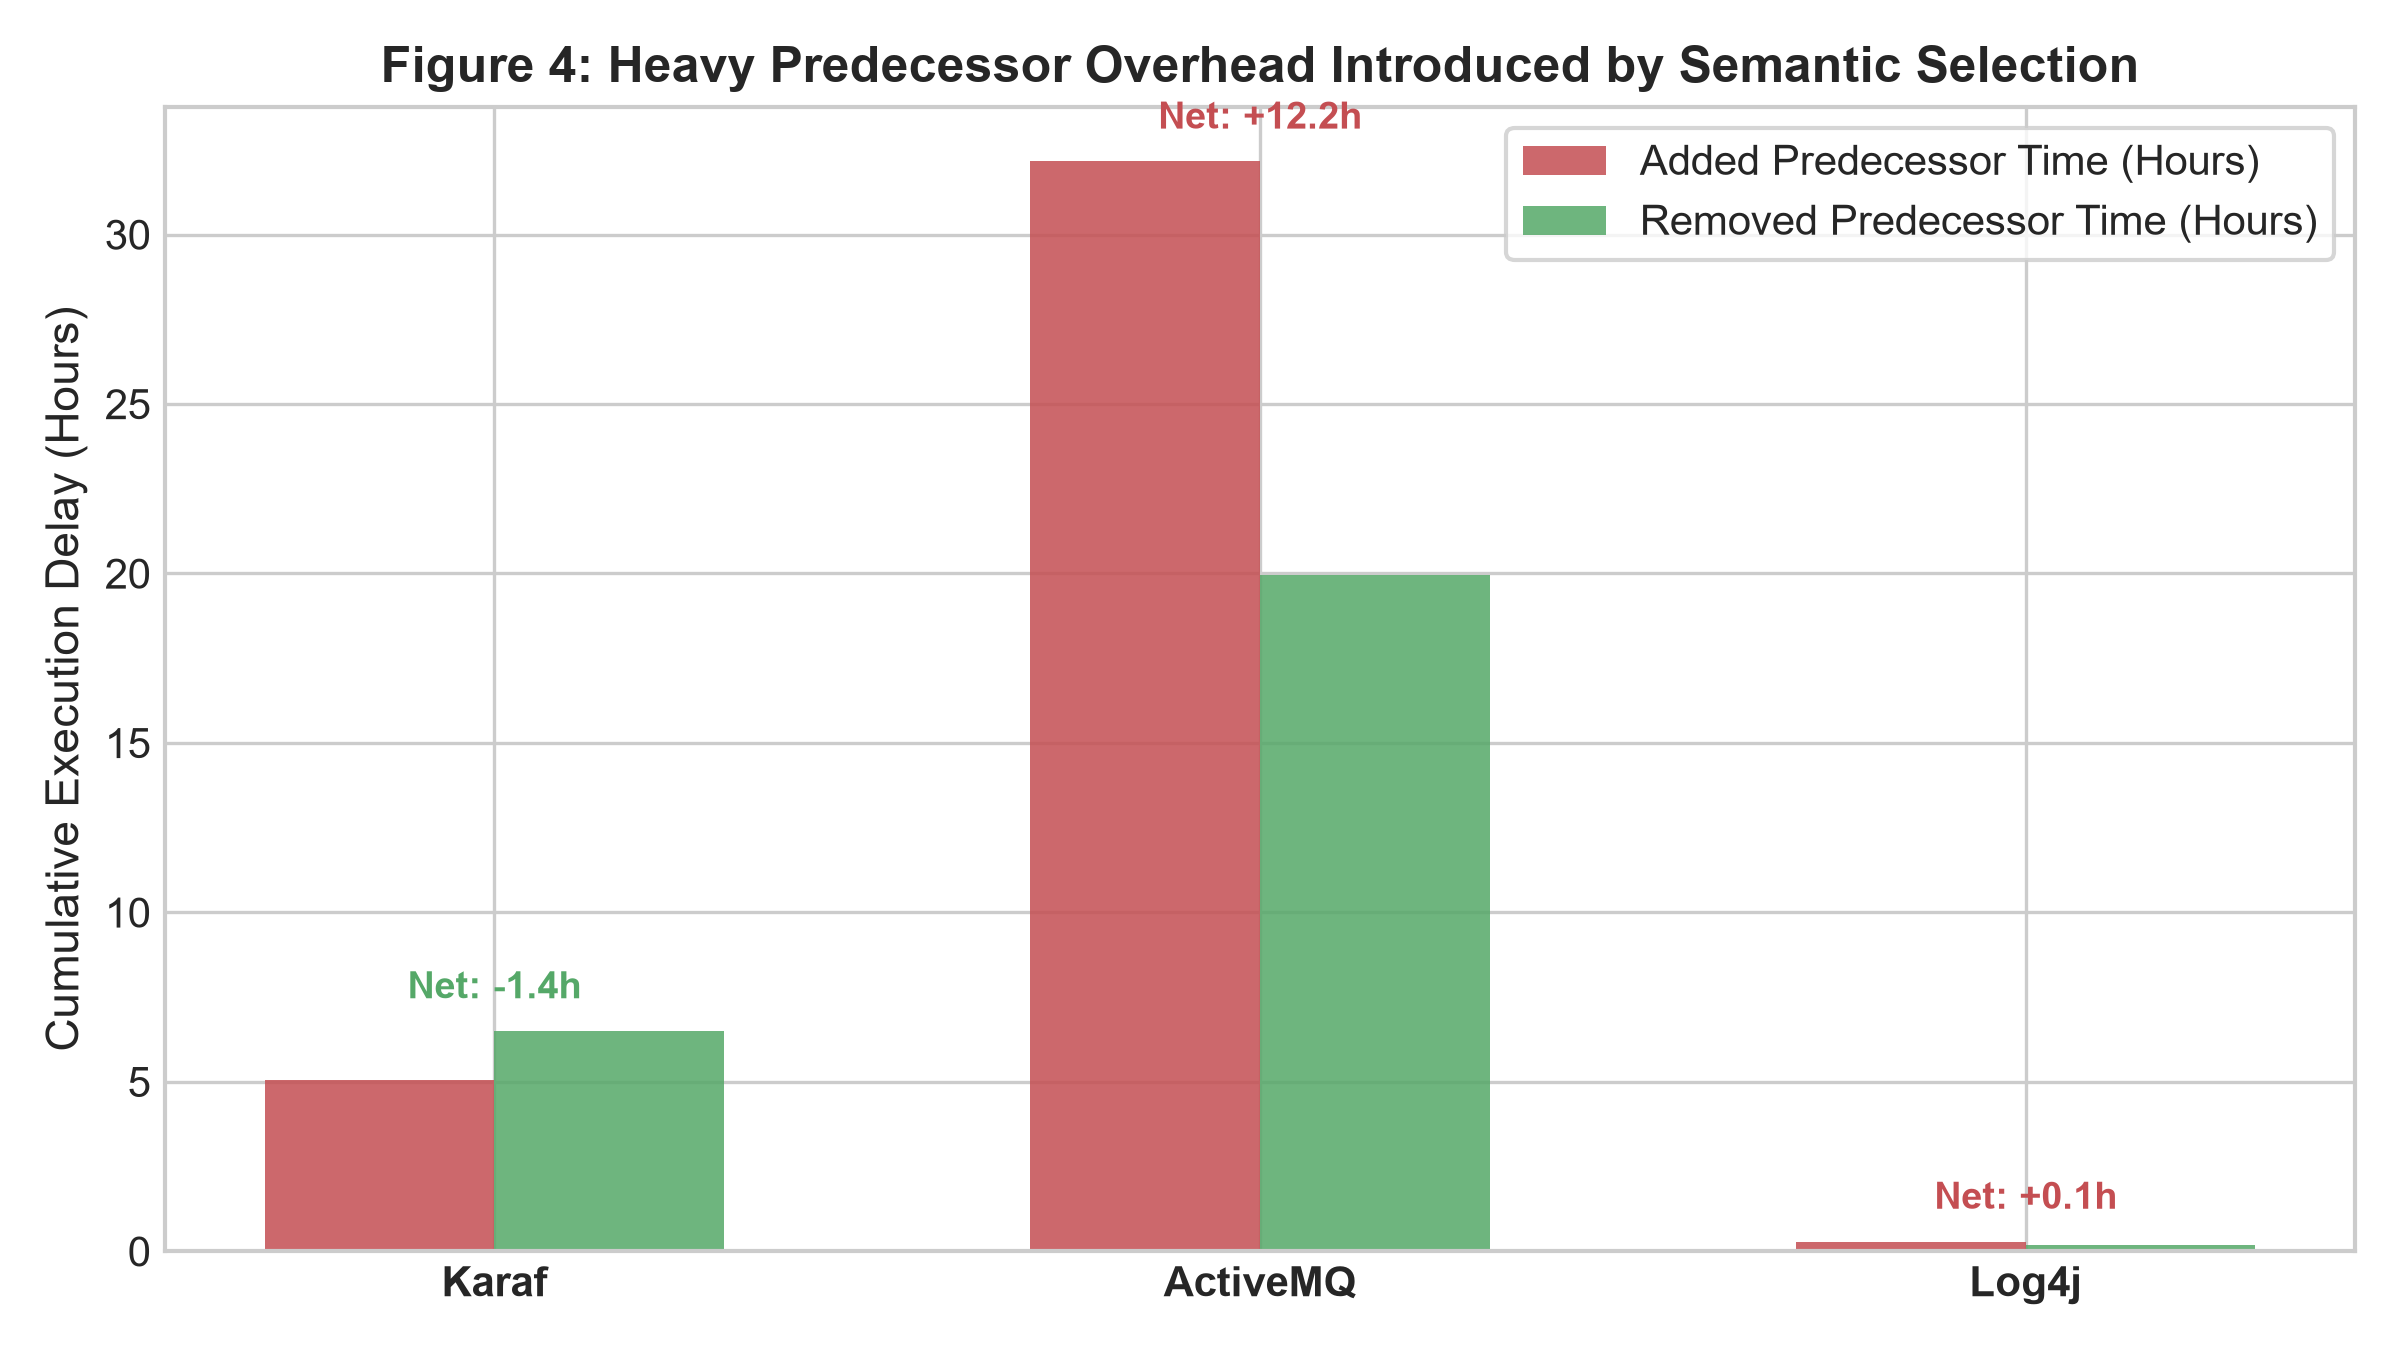
\includegraphics[width=0.85\textwidth]{Images/Figs/fig4_heavy_predecessors.png}
\caption{Phân rã độ trễ tích lũy ($T_{add}$, $T_{rem}$, $T_{net}$) do hiện tượng Heavy Predecessors}
\label{fig:heavy_predecessors}
\vspace{1mm}
\footnotesize{\textit{Nguồn hình vẽ: Tệp kết xuất đồ họa \texttt{reports/figures/fig4\_heavy\_predecessors.png}.}}
\end{figure}

% -----------------------------------------------------------------------------
\subsubsection{Các lớp kiểm thử đóng vai trò thủ phạm gây trễ điển hình}
\label{subsubsec:top_heavy_predecessors}

Phân tích chi tiết mức độ dịch chuyển cho thấy hiện tượng trễ tập trung vào một số lớp kiểm thử cụ thể có thời gian chạy dài:
\begin{itemize}
    % nguon: reports/stage11/forensic-analysis.json (dòng 319-320)
    \item Lớp kiểm thử \texttt{MQTTAutoNioTest} (ActiveMQ): Có thời gian thực thi trung bình từ 150 đến 250 giây. Trong thứ tự xếp hạng của HC-FALCON v1, bài test này xuất hiện làm Heavy Predecessor trong \textbf{102 lượt} (failure shifts) trải dài trên \textbf{38 trong tổng số 57 build lỗi} (66,7\%) của ActiveMQ.
    % nguon: reports/stage11/forensic-analysis.json (dòng 324)
    \item Lớp kiểm thử \texttt{StompAutoNioSslTest} (ActiveMQ): Xuất hiện làm Heavy Predecessor trong \textbf{76 lượt} trên hệ thống CI của ActiveMQ.
    % nguon: docs/BAO_CAO_TONG_HOP_DU_AN.md (dòng 462, 463)
    \item Tại Karaf: hai lớp kiểm thử \texttt{Spring43FeaturesTest} và \texttt{SystemCommandSecurityTest} lần lượt xuất hiện làm tiền nhiệm đứng trước các test phát hiện lỗi trong \textbf{42 lượt} và \textbf{40 lượt}.
    % nguon: docs/BAO_CAO_TONG_HOP_DU_AN.md (dòng 469)
    \item Lớp kiểm thử \texttt{RollingAppenderDirectWriteTest} (Log4j2): Xuất hiện làm tiền nhiệm gây trễ trong \textbf{24 lượt} tại Log4j2.
\end{itemize}

% =============================================================================
\subsection{Phân tích bóc tách các thành phần (Ablation Study)}
\label{subsec:ablation}

% TODO: Hiện tại trong kho dữ liệu chưa ghi nhận thực nghiệm bóc tách độc lập (ablation study) riêng rẽ cho từng hệ số phạt chi phí hay kịch bản cold-start độc lập. Mục này được tạm thời giữ nguyên cấu trúc nháp để bổ sung khi có dữ liệu.

Hiện tại, các thực nghiệm đối chứng bóc tách thành phần độc lập (như việc ngắt bỏ hoàn toàn hệ số chi phí hay cô lập tín hiệu ngữ nghĩa trong giai đoạn khởi động lạnh cold-start) chưa được hoàn thiện trên kho lưu trữ. Các phát hiện định lượng liên quan sẽ được bổ sung khi có dữ liệu thực nghiệm kiểm chứng độc lập.

% =============================================================================
\subsection{Tổng kết chương}
\label{subsec:experiments_summary}

Chương 4 đã báo cáo toàn diện các số liệu thực nghiệm thu được từ hai trục nghiên cứu:
\begin{enumerate}
    \item \textbf{Trên Defects4J (Trục 1):} Tái lập thuật toán FALCON trên 6 dự án phần mềm với điểm APFD trung bình đạt 0,7260 so với 0,7223 của bài báo gốc (sai lệch có dấu trung bình $+0,0037$, sai lệch tuyệt đối trung bình MAE đạt $0,0042$, sai lệch tuyệt đối lớn nhất là $0,0132$ tại Math). Thử nghiệm Bridge xác nhận việc bổ sung tiền xử lý mã nguồn và mặt nạ chú ý chuẩn ghi nhận mức chênh lệch $+0,0312$ APFD trên dự án Chart.
    \item \textbf{Trên CI thực tế (Trục 2):} Đánh giá trên 161 build lỗi tập phát triển cho thấy các biến thể HC-FALCON v1, hạn chế ngữ nghĩa, CNS-Greedy và UGCS v2 đều ghi nhận trung vị chênh lệch $\Delta\text{APFDc}$ mang dấu âm so với baseline \texttt{history\_cost}. Biến thể cuối UGCS v2 đạt tỷ lệ thắng từ 15,79\% đến 25,32\%, vi phạm cả Effect Gate và Runtime Gate, dẫn đến phán quyết dừng tại tập phát triển và tiếp tục niêm phong 100\% tập kiểm chứng gồm 142 build lỗi.
    \item \textbf{Về dữ liệu forensic và chi phí thực thi:} Định lượng hiện tượng Heavy Predecessors ghi nhận độ trễ ròng tích lũy $+39.099,3$ giây trên 161 build lỗi của HC-FALCON v1 (bình quân $+242,85$ s/build), trong đó lớp kiểm thử \texttt{MQTTAutoNioTest} xuất hiện làm tiền nhiệm gây trễ trong 102 lượt trên 38/57 build lỗi của ActiveMQ. Biến thể UGCS v2 cắt giảm $-9.631,3$ giây thời gian tiền nhiệm ròng tích lũy so với \texttt{history\_cost} (bình quân $-59,82$ s/build) nhưng vẫn có 72,05\% số build thua về $\Delta\text{APFDc}$.
\end{enumerate}

Toàn bộ các ý nghĩa phương pháp luận, sự khác biệt giữa hai môi trường kiểm thử và phân tích nguyên nhân cơ chế của các hiện tượng trên sẽ được thảo luận chi tiết tại Chương~\ref{sec:discussion}.

\section{Thảo luận}
\label{sec:discussion}

% Nội dung sẽ được triển khai chi tiết trong Phase 4 theo kế hoạch.


\newpage
\section*{Kết luận}
\addcontentsline{toc}{section}{Kết luận}
\label{sec:conclusion}


\newpage
\renewcommand{\refname}{Tài liệu tham khảo}
\bibliographystyle{ieeetr}
\addcontentsline{toc}{section}{Tài liệu tham khảo}
\bibliography{ref}

\newpage
\appendix
\addcontentsline{toc}{section}{Phụ lục}

\section*{Phụ lục A: Bảng đối chiếu mã nội bộ các giai đoạn (Stage)}
\addcontentsline{toc}{subsection}{Phụ lục A: Bảng đối chiếu mã nội bộ các giai đoạn}
\label{app:stages}

\begin{table}[H]
\centering
\small
\renewcommand{\arraystretch}{1.2}
\setlength{\tabcolsep}{4pt}
\begin{tabular}{|c|p{4.2cm}|p{8.2cm}|}
\hline
\textbf{Mã nội bộ} & \textbf{Tên mô tả chính thức} & \textbf{Nội dung kỹ thuật cốt lõi} \\
\hline
Stage 1 & Rà soát dữ liệu đầu vào và kiểm định khả thi & Kiểm tra toàn vẹn dữ liệu Defects4J, LRTS và mô hình UniXcoder \\
\hline
Stage 2 & Thiết lập môi trường thử nghiệm sơ bộ & Dựng pipeline chạy thử và các baseline đối chứng cơ sở \\
\hline
Stage 3 & Khảo sát thí điểm Karaf & Thử nghiệm mô phỏng trên tập Karaf exploratory \\
\hline
Stage 4 & Thiết kế kiến trúc và mô hình HC-FALCON v1 & Xây dựng hàm mục tiêu kết hợp Submodular và Bayes \\
\hline
Stage 5 & Trích xuất mã nguồn và tiền xử lý embedding & Trích xuất 1.155 test class LRTS và tạo vector UniXcoder \\
\hline
Stage 6 & Thử nghiệm mô hình cơ sở HC-FALCON v1 & Đánh giá hai biến thể \texttt{topic\_raw} và \texttt{normalized} trên LRTS \\
\hline
Stage 7 & Chẩn đoán nguyên nhân sâu và Heavy Predecessors & Phân tích 161 build lỗi và đo đạc độ trễ thêm vào $T_{\text{add}}$ \\
\hline
Stage 8 & Biến thể hạn chế ngữ nghĩa theo cửa sổ lịch sử & Thử nghiệm áp trần điểm lịch sử ($q \ge 0{,}95 q_{\max}$) \\
\hline
Stage 9 & Kiểm tra độ chuẩn xác kỹ thuật và tính toàn vẹn & Đảm bảo tính toán đúng và kiểm tra chống rò rỉ dữ liệu \\
\hline
Stage 10 & Tái lập độc lập FALCON trên Defects4J & Tái lập 6 dự án Defects4J và phân rã Bridge Chart A/B/C/D \\
\hline
Stage 11 & Biến thể CNS-Greedy và phân tích nguyên nhân & Chuẩn hóa chi phí vào hàm tham lam và đo forensic 161 build \\
\hline
Stage 12 & Biến thể UGCS v2 và đánh giá cổng quyết định & Thuật toán bảo vệ bất định 4 bước và phán quyết NO-GO chính thức \\
\hline
\end{tabular}
\caption{Bảng đối chiếu mã phân đoạn nội bộ với tên mô tả chính thức sử dụng trong báo cáo.}
\end{table}

\newpage
\section*{Phụ lục C: Mã nguồn minh họa thuật toán cốt lõi}
\addcontentsline{toc}{subsection}{Phụ lục C: Mã nguồn minh họa thuật toán cốt lõi}
\label{app:code}

Dưới đây là phần triển khai Python minh họa cho thuật toán xếp hạng UGCS v2 (\textit{Uncertainty-Guarded Cost-aware Semantic Greedy}) được tiền đăng ký tại Stage 12:

\begin{algorithm}[H]
\caption{Mô phỏng thuật toán UGCS v2 (Uncertainty-Guarded Cost-aware Semantic Greedy)}
\label{alg:ugcs_v2_code}
\begin{algorithmic}[1]
\Require Tập kiểm thử $V$, kernel tương đồng ngữ nghĩa $K$, lịch sử quan sát $\{h_t\}$, chi phí thực thi $\{c_t\}$
\Ensure Hoán vị thứ tự kiểm thử $\pi$
\State $p_t \leftarrow \text{EstimateBetaBernoulli}(h_t)$ \Comment{Ước lượng rủi ro lỗi tiên nghiệm Bayes}
\State $\text{conf}_t \leftarrow 1 - \frac{1}{\sqrt{N_t + 1}}$ \Comment{Hệ số tin cậy theo số lần quan sát}
\State $q_t \leftarrow \frac{p_t \cdot \text{conf}_t}{\sqrt{c_t}}$ \Comment{Chỉ số rủi ro - chi phí kết hợp}
\State $q_{\max} \leftarrow \max_{t \in V} q_t$
\State $V_{\text{top}} \leftarrow \{t \in V \mid q_t \ge (1 - \alpha) q_{\max}\}$ \Comment{Khoanh vùng ứng viên bất định}
\State $S \leftarrow \emptyset$, $\pi \leftarrow []$
\While{$V_{\text{top}} \setminus S \ne \emptyset$}
    \State $t^* \leftarrow \arg\max_{t \in V_{\text{top}} \setminus S} \left[ q_t + \lambda \cdot \frac{\Delta FL(t \mid S)}{n \cdot c_t} \right]$ \Comment{Tham lam nhận thức chi phí}
    \State $S \leftarrow S \cup \{t^*\}$
    \State $\pi.\text{append}(t^*)$
\EndWhile
\State $V_{\text{rest}} \leftarrow V \setminus S$
\State Sắp xếp $V_{\text{rest}}$ giảm dần theo $q_t$ (tie-breaking theo $c_t$ tăng dần)
\State Nối $V_{\text{rest}}$ vào cuối $\pi$
\State \Return $\pi$
\end{algorithmic}
\end{algorithm}


\end{document}
